%
% $RCSfile: cybol.tex,v $
%
% Copyright (c) 2002-2007. Christian Heller. All rights reserved.
%
% Permission is granted to copy, distribute and/or modify this document
% under the terms of the GNU Free Documentation License, Version 1.1 or
% any later version published by the Free Software Foundation; with no
% Invariant Sections, with no Front-Cover Texts and with no Back-Cover
% Texts. A copy of the license is included in the section entitled
% "GNU Free Documentation License".
%
% http://www.cybop.net
% - Cybernetics Oriented Programming -
%
% Version: $Revision: 1.1 $ $Date: 2007-07-17 20:02:36 $ $Author: christian $
% Authors: Christian Heller <christian.heller@tuxtax.de>
%

%
% Determine document class specifying the type of document.
%
% Hand over font size and side format.
%
%\documentclass[9pt,twoside]{tuxtax}
\documentclass[10pt,twoside]{tuxtax}

%
% Input hyphenation list.
%
%%
% $RCSfile: hyphenation.tex,v $
%
% Copyright (c) 2001-2004. Christian Heller. All rights reserved.
%
% No copying, altering, distribution or any other actions concerning this
% document, except after explicit permission by the author!
% At some later point in time, this document is planned to be put under
% the GNU FDL license. For now, _everything_ is _restricted_ by the author.
%
% http://www.cybop.net
% - Cybernetics Oriented Programming -
%
% http://www.resmedicinae.org
% - Information in Medicine -
%
% @author Christian Heller <christian.heller@tuxtax.de>
%

\hyphenation{abs-trac-tion}
\hyphenation{abs-trac-tions}
\hyphenation{ac-tu-ally}
\hyphenation{addi-tio-nally}
\hyphenation{ana-lyst}
\hyphenation{ana-ly-sis}
\hyphenation{an-cient}
\hyphenation{ap-pli-ca-tion}
\hyphenation{arche-types}
\hyphenation{aris-to-tle}
\hyphenation{at-tri-bute}
\hyphenation{avoi-da-ble}
\hyphenation{be-ing}
\hyphenation{binary}
\hyphenation{bran-ches}
\hyphenation{ca-te-go-ri-za-tion}
\hyphenation{client}
\hyphenation{com-po-nen-ti-za-tion}
\hyphenation{com-pu-ter}
\hyphenation{con-fi-gure}
\hyphenation{con-fi-gu-ra-tion}
\hyphenation{con-nec-ted}
\hyphenation{cri-ti-cised}
\hyphenation{cy-ber-ne-tics}
\hyphenation{cyboi}
\hyphenation{cybol}
\hyphenation{cybop}
\hyphenation{de-sign}
\hyphenation{des-cribe}
\hyphenation{des-cribed}
\hyphenation{de-ve-lop-ment}
\hyphenation{dis-crete}
\hyphenation{di-vide}
\hyphenation{do-main}
\hyphenation{dy-na-mic}
\hyphenation{dy-na-mics}
\hyphenation{ela-bo-ra-ted}
\hyphenation{ele-ments}
\hyphenation{en-gi-nee-ring}
\hyphenation{eng-lish}
\hyphenation{en-vi-ron-ment}
\hyphenation{ex-pert}
\hyphenation{fi-gure}
\hyphenation{fun-da-men-tal}
\hyphenation{func-tio-na-li-ty}
\hyphenation{hard-ware}
\hyphenation{hu-man}
\hyphenation{im-ple-men-ta-tion}
\hyphenation{imp-roved}
\hyphenation{in-he-rit}
\hyphenation{in-ter-pre-ter}
\hyphenation{java}
\hyphenation{know-ledge}
\hyphenation{lan-guage}
\hyphenation{li-ving}
\hyphenation{lo-gi-cal}
\hyphenation{machine}
\hyphenation{me-cha-nism}
\hyphenation{me-thods}
\hyphenation{na-ture}
\hyphenation{net-work}
\hyphenation{neu-ral}
\hyphenation{neu-ron}
\hyphenation{nu-me-rous}
\hyphenation{object}
\hyphenation{open}
\hyphenation{operating}
\hyphenation{ori-en-ted}
\hyphenation{over-come}
\hyphenation{prin-ci-ple}
\hyphenation{prin-ting}
\hyphenation{pro-ba-bi-lis-tic}
\hyphenation{pro-gram-ming}
\hyphenation{re-cog-nize}
\hyphenation{re-cog-nized}
\hyphenation{re-pre-sen-ta-tion}
\hyphenation{re-pre-sen-ting}
\hyphenation{re-u-sa-bi-li-ty}
\hyphenation{sci-ence}
\hyphenation{server}
\hyphenation{se-pa-ra-ted}
\hyphenation{se-pa-ra-tion}
\hyphenation{si-mi-lar}
\hyphenation{soft-ware}
\hyphenation{source}
\hyphenation{spe-cia-li-za-tion}
\hyphenation{sta-tic}
\hyphenation{sta-ti-cal-ly}
\hyphenation{sto-chas-tic}
\hyphenation{stone-on-stone}
\hyphenation{struc-ture}
\hyphenation{strug-gling}
\hyphenation{su-per-flu-ous}
\hyphenation{sup-ply-ing}
\hyphenation{sys-tem}
\hyphenation{tes-ting}
\hyphenation{thin-king}
\hyphenation{un-en-li-vened}
\hyphenation{un-fa-vou-ra-ble}
\hyphenation{un-sa-tis-fy-ing}
\hyphenation{va-ry-ing}
\hyphenation{weigh-ted}


%
% Define text macros.
%
\def\placemacro{Ilmenau}
\def\datemacro{2007-07-06}
\def\authormacro{Christian Heller}

%
% Enable special indexing commands.
% Generate contents, glossary and memo entries.
%
% Required package: makeidx
%
\makeindex

%
% This document describes the Cybernetics Oriented Language (CYBOL).
%
% Author: Christian Heller <christian.heller@tuxtax.de>
%
\begin{document}
    % Set sans serif font.
    \sffamily
    % Set page numbering to roman numbers.
    \pagenumbering{roman}
    %
% $RCSfile: cover.tex,v $
%
% Copyright (C) 2002-2008. Christian Heller.
%
% Permission is granted to copy, distribute and/or modify this document
% under the terms of the GNU Free Documentation License, Version 1.1 or
% any later version published by the Free Software Foundation; with no
% Invariant Sections, with no Front-Cover Texts and with no Back-Cover
% Texts. A copy of the license is included in the section entitled
% "GNU Free Documentation License".
%
% http://www.cybop.net
% - Cybernetics Oriented Programming -
%
% http://www.resmedicinae.org
% - Information in Medicine -
%
% Version: $Revision: 1.1 $ $Date: 2008-08-19 20:41:06 $ $Author: christian $
% Authors: Christian Heller <christian.heller@tuxtax.de>
%

%
% Defines the title page.
%
% \title and \author (and optionally \date) must be specified!
%
% Sets the page style of the first page to empty
% that is no header or footer will be shown.
%
\begin{titlepage}
    \title{
        Cybernetics Oriented Programming\\
        (CYBOP)\\
        \vspace{1cm}
        % \textmd sets medium weight (default), which is the opposite of boldface.
        \normalsize{\textmd{An Investigation on the Applicability of Inter-Disciplinary Concepts\\
            to Software System Development\\}}
    }
    \author{
        \date{
        }
    }
\end{titlepage}

    \maketitle
    % Avoid header, footer and page number.
    \thispagestyle{empty}
    %
% $RCSfile: title.tex,v $
%
% Copyright (c) 2001-2004. Christian Heller. All rights reserved.
%
% No copying, altering, distribution or any other actions concerning this
% document, except after explicit permission by the author!
% At some later point in time, this document is planned to be put under
% the GNU FDL license. For now, _everything_ is _restricted_ by the author.
%
% http://www.cybop.net
% - Cybernetics Oriented Programming -
%
% http://www.resmedicinae.org
% - Information in Medicine -
%
% @author Christian Heller <christian.heller@tuxtax.de>
%

\title{A new Pattern Systematics}
\author{
    Christian Heller \(<\)christian.heller@tu-ilmenau.de\(>\)\\
    Detlef Streitferdt \(<\)detlef.streitferdt@tu-ilmenau.de\(>\)\\
    Ilka Philippow \(<\)ilka.philippow@tu-ilmenau.de\(>\)
}
\institute{Technical University of Ilmenau\\
    Faculty for Computer Science and Automation\\
    Institute for Theoretical and Technical Informatics\\
    PF 100565, Max-Planck-Ring 14, 98693 Ilmenau, Germany\\
    http://www.tu-ilmenau.de, fon: +49-3677-69-1230, fax: +49-3677-69-1220 \vspace*{0.5cm}
}

    \newpage{\pagestyle{empty}\clearpage}
    \thispagestyle{empty}
    %
% $RCSfile: copyright.tex,v $
%
% Copyright (c) 2002-2007. Christian Heller. All rights reserved.
%
% Permission is granted to copy, distribute and/or modify this document
% under the terms of the GNU Free Documentation License, Version 1.1 or
% any later version published by the Free Software Foundation; with no
% Invariant Sections, with no Front-Cover Texts and with no Back-Cover
% Texts. A copy of the license is included in the section entitled
% "GNU Free Documentation License".
%
% http://www.cybop.net
% - Cybernetics Oriented Programming -
%
% Version: $Revision: 1.2 $ $Date: 2007-08-01 13:59:00 $ $Author: christian $
% Authors: Christian Heller <christian.heller@tuxtax.de>
%

\small{Cataloging-in-Publication Data\\\\
    \authormacro.\\
    \titlemacro:\\
    \subtitlemacro\\
    \versionmacro\\
    \placemacro: Tux Tax, 2007%\\
%    ISBN-10: 3-9810898-0-4 xxx EDIT xxx\\
%    ISBN-13: 978-3-9810898-0-6 xxx EDIT xxx
}\\

\small{Information about this specification\\
    http://www.cybop.net, http://www.tuxtax.de}

\vspace{4cm}

\small{Copyright \textcopyright\ 2002-2007. \authormacro. All rights reserved.}

%> \small{Translation: Christian Heller}\\ %\"Ubersetzung:
%\small{Sponsoring Editor: ??}\\ %Lektorat:
%\small{Acquisitions Editor: ??}\\
%\small{Marketing Manager: ??}\\
%\small{Marketing Assistant: ??}\\
%\small{Editorial Assistant: ??}\\
%\small{Editorial/ Production Supervision: ??}\\
%\small{Production Editor: Christian Heller}\\ %Produktion:
%\small{Production Service: ??}\\ %Produktion:
%\small{Manuscript Editor: ??}\\
%\small{Interior Illustration: ??}\\
%\small{Interior Design: ??}\\
%\small{Cover Illustration: TSAMEDIEN, D\"usseldorf}\\ %Umschlaggrafik:
%\small{Cover Design: Christian Heller}\\ %Umschlaggestaltung:
%\small{Print Buyer: ??}\\
%\small{Project Coordinator: ??}\\
%> \small{Typesetting: Christian Heller, set in Times 9.5 pt font with \LaTeX\ using Kile under Linux}\\ %Satz:
%\small{Cover Printing: ??}\\
%\small{Printing and Binding: Offizin Andersen Nex\"o, Leipzig/ Zwenkau} %Belichtung, Druck und Bindung:

\small{Permission is granted to copy, distribute and/or modify this document
    under the terms of the GNU Free Documentation License, Version 1.2
    or any later version published by the Free Software Foundation;
    with no Invariant Sections, with no Front-Cover Texts and with no
    Back-Cover Texts. A copy of the license is included in the section
    entitled "GNU Free Documentation License".}

\small{Trademark Credits\\
    Most of the software-, hardware- and product names used in this document
    are also trademarks or registered trademarks of their respective owners.
%    Adobe is a trademark of Adobe Systems, Incorporated.\\
%    AIX is a trademark of International Business Machines Corporation.\\
%    Arial\textregistered\ is a registered trademark of the Monotype Corporation in the United States and other countries.\\
%>    CICS is a trademark of International Business Machines Corporation.\\
%    CICS/ESA is a trademark of International Business Machines Corporation.\\
%    CorelDRAW\texttrademark\ is a trademark or registered trademark of Corel Corporation or Corel Corporation Limited.\\
%>    DB2 is a trademark of International Business Machines Corporation.\\
%    DFSMS is a trademark of International Business Machines Corporation.\\
%    DFSORT is a trademark of International Business Machines Corporation.\\
%    Energy Star\textregistered\ and the Energy Star logo\textregistered\ are registered marks of the United States Environmental Protection Agency in the United States and other countries. Details on the proper use of the marks are explained in the "Guidelines for Proper use of the Energy Star\textregistered\ Name and International Logo".\\
%>    Ethernet is a registered trademark of Xerox Corporation.\\
%>    IBM\textregistered\ is a registered trademark of International Business Machines Corporation.\\
%    IBM Warp Server\textregistered\ is a registered trademark of International Business Machines Corporation.\\
%    IMS is a trademark of International Business Machines Corporation.\\
%    IMS/ESA is a trademark of International Business Machines Corporation.\\
%>    Intel is a registered trademark of Intel Corporation in the United States and other countries.\\
%>    Java\texttrademark\ and all Java-based trademarks are trademarks of Sun Microsystems, Inc. in the United States and other countries.\\
%    Language Environment is a trademark of International Business Machines Corporation.\\
%>    Microsoft\textregistered\ is a registered trademark of Microsoft Corporation in the United States and other countries.\\
%    MS Windows\textregistered\ is a registered trademark of Microsoft Corporation in the United States and other countries.\\
%    MS-DOS\textregistered\ is a registered trademark of Microsoft Corporation in the United States and other countries.\\
%    MVS is a trademark of International Business Machines Corporation.\\
%    Netscape is a trademark of Netscape Communications Corporation in the United States and other countries.\\
%    Netscape Navigator is a trademark of Netscape Communications Corporation in the United States and other countries.\\
%    Netware\textregistered\ is a registered trademark of Novell Corporation.\\
%    Novell\textregistered\ is a registered trademark of Novell Corporation.\\
%    OpenEdition is a trademark of International Business Machines Corporation.\\
%    Opera\texttrademark\ is a trademark of Opera Software ASA.\\
%    Operating System/2\textregistered\ (OS/2) is a registered trademark of International Business Machines Corporation.\\
%    *Pantone, Inc. is a check-standard trademark for color.\\
%>    Pentium is a registered trademark of Intel Corporation in the United States and other countries.\\
%>    PostScript is a trademark of Adobe Systems, Incorporated.\\
%    RACF is a trademark of International Business Machines Corporation.\\
%    System/390 is a trademark of International Business Machines Corporation.\\
%>    Unicode is a trademark of the Unicode Consortium.\\
%>    UNIX\textregistered\ is a registered trademark of The Open Group in the United States and other countries.\\
%    VisualAge is a trademark of International Business Machines Corporation.\\
%>    Windows\textregistered\ is a registered trademark of Microsoft Corporation in the United States and other countries.\\
%    Windows NT\textregistered\ is a registered trademark of Microsoft Corporation in the United States and other countries.\\
%    z/OS is a trademark of International Business Machines Corporation.\\
%>    Other company-, product- or service names may be the trademarks or service marks of others.\\
}

\small{Donations\\
    Companies using CYBOP ideas, CYBOL or CYBOI on a grand scale are asked to
    notify the author \(<\)christian.heller@tuxtax.de\(>\) and to consider
    donating some of their sales revenues, which will be used exclusively for
    the CYBOP and Res Medicinae free software projects.}

%\small{Text printed on recycled and acid-free paper.}

\small{Made in Germany, Europe, Planet Earth}

    \newpage{\pagestyle{empty}\cleardoublepage}
    % Avoid header, footer and page number.
    \thispagestyle{empty}
    %
% $RCSfile: dedication.tex,v $
%
% Copyright (C) 2002-2008. Christian Heller.
%
% Permission is granted to copy, distribute and/or modify this document
% under the terms of the GNU Free Documentation License, Version 1.1 or
% any later version published by the Free Software Foundation; with no
% Invariant Sections, with no Front-Cover Texts and with no Back-Cover
% Texts. A copy of the license is included in the section entitled
% "GNU Free Documentation License".
%
% http://www.cybop.net
% - Cybernetics Oriented Programming -
%
% http://www.resmedicinae.org
% - Information in Medicine -
%
% Version: $Revision: 1.1 $ $Date: 2008-08-19 20:41:06 $ $Author: christian $
% Authors: Christian Heller <christian.heller@tuxtax.de>
%

\vspace*{3cm}
\begin{center}
    To all kind-hearted People who contribute to Humanity;\\
    against Those whose only Aim in Life is to amass Money
\end{center}

    \newpage{\pagestyle{empty}\cleardoublepage}
    \tableofcontents
    \newpage{\pagestyle{empty}\cleardoublepage}
    % Set roman font.
    \rmfamily
    %
% $RCSfile: preface.tex,v $
%
% Copyright (C) 2002-2008. Christian Heller.
%
% Permission is granted to copy, distribute and/or modify this document
% under the terms of the GNU Free Documentation License, Version 1.1 or
% any later version published by the Free Software Foundation; with no
% Invariant Sections, with no Front-Cover Texts and with no Back-Cover
% Texts. A copy of the license is included in the section entitled
% "GNU Free Documentation License".
%
% http://www.cybop.net
% - Cybernetics Oriented Programming -
%
% http://www.resmedicinae.org
% - Information in Medicine -
%
% Version: $Revision: 1.1 $ $Date: 2008-08-19 20:41:08 $ $Author: christian $
% Authors: Christian Heller <christian.heller@tuxtax.de>
%

\chapter*{Preface\markboth{Preface}{Preface}}
\label{preface_heading}
\addcontentsline{toc}{chapter}{Preface}

\begin{flushright}
    \textsl{
        I slept and dreamt that Life was Joy.\\
        I awoke and saw that Life was Service.\\
        I acted and behold, Service was joy.
    }\\
    \textsc{Rabindranath Tagore}
\end{flushright}

%
% $RCSfile: prologue.tex,v $
%
% Copyright (C) 2002-2008. Christian Heller.
%
% Permission is granted to copy, distribute and/or modify this document
% under the terms of the GNU Free Documentation License, Version 1.1 or
% any later version published by the Free Software Foundation; with no
% Invariant Sections, with no Front-Cover Texts and with no Back-Cover
% Texts. A copy of the license is included in the section entitled
% "GNU Free Documentation License".
%
% http://www.cybop.net
% - Cybernetics Oriented Programming -
%
% http://www.resmedicinae.org
% - Information in Medicine -
%
% Version: $Revision: 1.2 $ $Date: 2008-09-07 15:36:07 $ $Author: christian $
% Authors: Christian Heller <christian.heller@tuxtax.de>
%

\section*{Prologue}
\label{prologue_heading}
%\addcontentsline{toc}{section}{Prologue}

To me, basically, there are two ways to deal with a scientific subject:

\begin{enumerate}
    \item The deepened investigation on a special area aiming to find
        completely new phenomenons
    \item The systematic subsumption of multiple known aspects of one or many
        disciplines aiming to find new cross-correlations and ideas
\end{enumerate}

Both approaches may lead to new theories, methods and concepts. And both may use
laboratory trials to find and prove their theories. This work follows the second
approach. The idea behind is, simply spoken, to steal ideas from nature and
various fields of science, and to apply them to software design.

\emph{Laboratory Trials} are what \emph{Coding} is in informatics -- experiment
and proof of operability, at the same time. Some information scientists have
the opinion that coding weren't \emph{scientific} enough and not necessary to
create new theories or to achieve good results. I doubt this. In my opinion,
there are things that can only be found when actually implementing ideas in a
computer language. And in the end, a theory is worth much more when having been
proven in practice. This document contains proven ideas that were growing in my
mind over the last few years, while dealing with topics such as:

\begin{itemize}
    \item[-] Structured- and Procedural Programming
    \item[-] Object Oriented Programming
    \item[-] Design Patterns and Frameworks
    \item[-] Component Based Design and Agents
    \item[-] Ontology Structured Domain Knowledge
    \item[-] Document- and User Interface Markup
    \item[-] Persistence Mechanisms
    \item[-] System Communication
    \item[-] Operating System Concepts
\end{itemize}

The usage of typical buzzwords could not quite be avoided in this work, yet do
I hope that the ideas and results are nevertheless explained straightforward and
well enough to be really useful to some other developers out there.

This document claims to be an \emph{Academic Paper}. To all practitioners who do
not want to read it for that reason, I would like to point out that each and
every concept in it arose from practice, that is coding. Like most developers,
I started up with only a few lines of code in one Java class, later extended to
more classes, a whole framework and so on. Whenever I stumbled over difficulties,
I thought through and improved my current design by applying patterns recommended
by several software development Gurus. It was only when I realised that even
those concepts were not sufficient, that I made up my own. They are entitled
\emph{Cybernetics Oriented Programming} (CYBOP), because most ideas behind them
stem from nature.

Finally, this document has become my thesis, written to earn a doctorate
(Dr.-Ing./ PhD) in Informatics/ Software Engineering. You may wonder why I
release it under the \emph{Free Documentation License} (FDL). Well, I'm a full
supporter of the idea of \emph{Free Knowledge}, \emph{Free Software}, a
\emph{Society free of Patents} which are only hindering its development. There
are three reasons that have contributed to my decision:

\begin{enumerate}
    \item Hope to get helpful \emph{Feedback} from readers
    \item Trust in the scientific \emph{Fairness} of colleagues, worldwide, to
        properly reference this document even though it is licensed under the FDL
    \item Wish to contribute to the open source movement \emph{now} (and not in
        some years when the document might reach a more stable version), to
        speed up its successful development
\end{enumerate}

This is a growing document undergoing steady development. It is not and doesn't
claim to be free of errors nor to contain the only possible way for application
system development. So, if you find errors of whatever kind or have any helpful
ideas or constructive criticism, then please contribute them to
\(<\)christian.heller@tuxtax.de\(>\) or to the CYBOP developers mailing list
\(<\)cybop-developers@lists.berlios.de\(>\)!

%
% $RCSfile: scientific_progress.tex,v $
%
% Copyright (C) 2002-2008. Christian Heller.
%
% Permission is granted to copy, distribute and/or modify this document
% under the terms of the GNU Free Documentation License, Version 1.1 or
% any later version published by the Free Software Foundation; with no
% Invariant Sections, with no Front-Cover Texts and with no Back-Cover
% Texts. A copy of the license is included in the section entitled
% "GNU Free Documentation License".
%
% http://www.cybop.net
% - Cybernetics Oriented Programming -
%
% http://www.resmedicinae.org
% - Information in Medicine -
%
% Version: $Revision: 1.1 $ $Date: 2008-08-19 20:41:08 $ $Author: christian $
% Authors: Christian Heller <christian.heller@tuxtax.de>
%

\section*{Scientific Progress}
\label{scientific_progress_heading}
%\addcontentsline{toc}{section}{Scientific Progress}

An \emph{Abstraction} allows to capture the real world by representing it in
simplified models. Such models contain only the essential aspects of a special
domain. Any unimportant nuances, in the considered context, are neglected.
Correct abstract models is what makes science easy. Good science \emph{can} be
\emph{easy}. If it is not, then probably either:

\begin{itemize}
    \item[-] there is a \emph{mistake} in the model
    \item[-] it is not fully \emph{understood} by the scientist him/ herself
    \item[-] the explaining person wants to \emph{keep back} knowledge, making
        others look clueless
\end{itemize}

One of the biggest hindrances to scientific progress is too much or false
respect for existing solutions. No theory/ model/ concept is ever finished;
no document/ software/ product is ever fully completed. There is always room
for improvements. In the end, it is all just a person's subjective perception
and an arbitrary, abstract extract of the real world.

It is always worth reviewing and questionning everything in depth, again and
again. Standstill means regress. The best example showing how to work around
these criticisms is the \emph{Free and Open Source Software} (FOSS) movement
where all the time, existing solutions are rewritten, to be improved.

%
% $RCSfile: software_patents.tex,v $
%
% Copyright (C) 2002-2008. Christian Heller.
%
% Permission is granted to copy, distribute and/or modify this document
% under the terms of the GNU Free Documentation License, Version 1.1 or
% any later version published by the Free Software Foundation; with no
% Invariant Sections, with no Front-Cover Texts and with no Back-Cover
% Texts. A copy of the license is included in the section entitled
% "GNU Free Documentation License".
%
% http://www.cybop.net
% - Cybernetics Oriented Programming -
%
% http://www.resmedicinae.org
% - Information in Medicine -
%
% Version: $Revision: 1.1 $ $Date: 2008-08-19 20:41:08 $ $Author: christian $
% Authors: Christian Heller <christian.heller@tuxtax.de>
%

\section*{Software Patents}
\label{software_patents_heading}
%\addcontentsline{toc}{section}{Software Patents}

This work is about software. Software abstracts the real world, its items and
processes, and it can store these information and their relations which make up
actual \emph{Knowledge}. In the modern, so-called \emph{Information Society},
it becomes more and more important to have \emph{free} access to external
knowledge. This is an \emph{essential} human right and will decide about the
future living quality of people.

So much the important it is to \emph{prohibit} the application of patents to
software! They make an exclusive club of large companies own the rights on
banal, ordinary, day-to-day algorithms and methods that many people use. And,
they thereby kill any new ideas and hinder research efforts that depend on
these basic algorithms. If \emph{Software Patents} and patents on
\emph{Computer Implemented Inventions} (CII) got introduced, any free software
developer and especially \emph{Small- and Medium Sized Enterprises} (SME), the
driving force of innovation, could not unfold their full potential anymore,
since much of their time and effort would then have to go into patent inquiries
and costly legal disputes.

Software patents are dangerous for the free development of thoughts! Certain
lobbies exert an increasing influence on politics and push members of
parliaments to agitate and vote in their interest. Since probably every reader
of this document has an interest in informatics, every reader is also affected
by the software patent enforcement. But everybody can do something about it,
not only in Europe! Express your protest and sign the petition at \cite{ffii}!

%
% $RCSfile: free_publishing.tex,v $
%
% Copyright (C) 2002-2008. Christian Heller.
%
% Permission is granted to copy, distribute and/or modify this document
% under the terms of the GNU Free Documentation License, Version 1.1 or
% any later version published by the Free Software Foundation; with no
% Invariant Sections, with no Front-Cover Texts and with no Back-Cover
% Texts. A copy of the license is included in the section entitled
% "GNU Free Documentation License".
%
% http://www.cybop.net
% - Cybernetics Oriented Programming -
%
% http://www.resmedicinae.org
% - Information in Medicine -
%
% Version: $Revision: 1.1 $ $Date: 2008-08-19 20:41:06 $ $Author: christian $
% Authors: Christian Heller <christian.heller@tuxtax.de>
%

\section*{Free Publishing}
\label{free_publishing_heading}
%\addcontentsline{toc}{section}{Free Publishing}

Reputation in the scientific world strongly depends on the number of
publications in scientific journals, conference proceedings, magazines etc., of
which some have greater kudos, some less. A \emph{Philosophiae Doctor} (PhD)
student, for example, is expected to publish in some of the \emph{acknowledged}
journals, in order to be conferred a doctorate. The grant of project fundings
by local-, national- or \emph{European Union} (EU) governements and sponsorship
of a professor's department at university depend on it as well. Some unfair
practices and shortcomings of the current system of publication shall therefore
be mentioned here. There are at least four disadvantages of publishing in
scientific journals. An author:

\begin{itemize}
    \item is almost always forced to assign his copyright to the publisher;
    \item has very little chance of publishing completely new ideas, since
        evaluators (which are to guarantee a certain \emph{scientific level})
        sieve those which seem too crazy or are unknown to them and do not
        match state-of-the-art science, so that really new ideas can hardly
        become popular in this way;
    \item has to wait many months before being informed about article
        acceptance, sometimes further months to presentation at a conference
        and yet more months until a journal/ proceedings are finally available
        -- which, besides the unfine delay, is enough time for an evaluator to
        adapt the best ideas and publish them in a modified form before;
    \item and everyone else have to pay money for receiving journals (even for
        the one containing the author's own work), or become a member of
        certain scientific societies for some discount -- which means that the
        work is not freely accessible.
\end{itemize}

Further, there is something often labelled \emph{Citation Mafia}. Whether an
article gets published in a journal or not depends on it being accepted by a
number of reviewers (normally three). In order to avoid personal battles, the
article author never gets to know the evaluators' names or proficiency and has
to blindly rely on the \emph{good taste} of a conference's program committee.
However, evaluators, although tied to ethical standards, often seem to have
their list of \emph{friends} or seem to just prefer authors who have already
published elsewhere, leading to circles of scientists citing each other, quite
independent from the quality of their papers. Logically, also here, there are a
number of disadvantages:

\begin{itemize}
    \item Young scientists have a hard life and need a long time for getting
        their articles accepted, independent from how innovative they are.
    \item Mafioso scientists often warm up old stories or deliver well-formulated,
        but rubbish articles not earning the predicate \emph{scientific}.
\end{itemize}

Don't ask for proof -- I don't have it. But almost everybody in the scientific
business knows about these issues. Unfortunately, only few people \cite{jobb}
talk about- or try to change them. Obviously, many scientists prefer to either
play the same old game or are scared of personal disadvantages. However, it
feels like increasingly more researchers, in particular the new generation,
become aware that these drawbacks hinder scientific progress and new solutions
need to be found. Well, there is free online journals such as the
\emph{Journal of Free and Open Source Medical Computing} (JOSMC) \cite{josmc}
or the \emph{BioMed Central} (BMC) \cite{bmc} publisher, where research
articles are: \textit{free to access immediately, peer reviewed,
citation-tracked \ldots}

Although this document cannot deliver solutions to the above-mentioned
problems, it mentioned those to inform the reader and spur further discussion.
Supportive actions in this process would be that:

\begin{itemize}
    \item scientists acknowledge no-cost entry open source conferences like
        LinuxTag \& Co. \cite{linuxtag} as alternatives to traditional ones
    \item professors more readily accept citations of free knowledge sources
        such as Wikipedia \cite{wikipedia} in scientific works of their students
    \item students and scientists publish their works (code and documentation)
        under open source licenses
\end{itemize}

%
% $RCSfile: new_science.tex,v $
%
% Copyright (C) 2002-2008. Christian Heller.
%
% Permission is granted to copy, distribute and/or modify this document
% under the terms of the GNU Free Documentation License, Version 1.1 or
% any later version published by the Free Software Foundation; with no
% Invariant Sections, with no Front-Cover Texts and with no Back-Cover
% Texts. A copy of the license is included in the section entitled
% "GNU Free Documentation License".
%
% http://www.cybop.net
% - Cybernetics Oriented Programming -
%
% http://www.resmedicinae.org
% - Information in Medicine -
%
% Version: $Revision: 1.1 $ $Date: 2008-08-19 20:41:07 $ $Author: christian $
% Authors: Christian Heller <christian.heller@tuxtax.de>
%

\section*{New Science}
\label{new_science_heading}
%\addcontentsline{toc}{section}{New Science}

It was end of October 2004 that I discovered Stephen Wolfram's book
\emph{A New Kind of Science} \cite{wolfram} (published in 2002), through a link
in Wikipedia \cite{wikipedia}. By that time, I was already heavily writing on
my own work.

During those years of thinking about software systems, nature, the universe --
I felt pretty similar to how Wolfram describes it in the preface of his book.
Starting with an inspection of state-of-the-art techniques, diving deeper and
deeper into several topics, I soon realised that they all could not deliver a
\emph{coherent}, \emph{conclusive} solution to software modelling. Each had its
own drawbacks that made workarounds necessary. And, the more I dived into the
different technologies, the more complex, complicated, intransparent they got
-- but still, none seemed to provide an \emph{overall} solution.

It was only when I got more and more distance to existing solutions and moved
away from current thinking, towards a more universal approach and a view at
software systems through the eyes of nature, that I found the basic principles
described in this work.

Now, after having read \emph{A New Kind of Science}, I am glad that Wolfram did
not already write down everything I want to say, so that there is something left
for me to contribute, by delivering this work :-) There is one difference that
soon became obvious to me: Wolfram argues, that it is possible to study the
abstract world of simple programs, and take lessons from what kinds of things
occur there and have them in mind when investigating natural systems
\cite{wikipedia}. My work follows the exact opposite way, in that it observes
phenomenons of nature and concepts used in other sciences, and tries to apply
them to the design of software systems.

This is \emph{not} to say that \emph{CYBOP} does provide \emph{the} overall
solution. But what it surely wants to reach is to encourage people to think in
more general terms, across disciplines, to possibly find new concepts. And for
that, this work hopes to deliver some ideas. And I certainly do hope that the
more you, as readers, think about these ideas, the more sense they will make to
you, too.

%
% $RCSfile: stylistic_means.tex,v $
%
% Copyright (c) 2002-2007. Christian Heller. All rights reserved.
%
% Permission is granted to copy, distribute and/or modify this document
% under the terms of the GNU Free Documentation License, Version 1.1 or
% any later version published by the Free Software Foundation; with no
% Invariant Sections, with no Front-Cover Texts and with no Back-Cover
% Texts. A copy of the license is included in the section entitled
% "GNU Free Documentation License".
%
% http://www.cybop.net
% - Cybernetics Oriented Programming -
%
% Version: $Revision: 1.1 $ $Date: 2007-07-17 20:02:36 $ $Author: christian $
% Authors: Christian Heller <christian.heller@tuxtax.de>
%

\section*{Stylistic Means and Notation}
\label{stylistic_means_heading}
%\addcontentsline{toc}{section}{Stylistic Means and Notation}

The language of choice in this document is \emph{British English}, more
precisely known as \emph{Commonwealth English}. Exceptions are citations or
proper names like \emph{Unified Modeling Language}, stemming from
\emph{American English} sources. (In Oxford English, \emph{Modelling} would be
written with double letter \emph{l}). I am thinking about writing a
\emph{German} version of this document, but am not sure if it will be worth the
effort. If you as reader are interested in a translation, send me a short note!
The more emails I receive, the more convinced I will be.

% Als Autor dieser Arbeit konnte ich mir die Freiheit nehmen, viele Textpassagen
% nicht wortgetreu, sondern vielmehr sinngem�� aus der englischen Originalfassung
% zu �bersetzen. Fachbegriffe aus der Computerwelt wurden in Englisch belassen,
% um keine Zweideutigkeiten und redundante Abk�rzungen entstehen zu lassen.

Correctly, masculine \emph{and} feminine forms are used in a work. When
describing a patient's record, for example, one would write: \textit{his or her
record}. In order to improve readability, and exclusively because of this
reason, only masculine forms are used in this work.

Pieces of software source code are displayed in \texttt{Typewriter Typeface}.
Emphasised words are \emph{italicised}.

Footnotes are not used on purpose. In my opinion, they only interrupt the
flow-of-reading. Remarks are placed in context instead, sometimes enclosed in
parentheses.

%
% $RCSfile: acknowledgements.tex,v $
%
% Copyright (c) 2001-2004. Christian Heller. All rights reserved.
%
% No copying, altering, distribution or any other actions concerning this
% document, except after explicit permission by the author!
% At some later point in time, this document is planned to be put under
% the GNU FDL license. For now, _everything_ is _restricted_ by the author.
%
% http://www.cybop.net
% - Cybernetics Oriented Programming -
%
% http://www.resmedicinae.org
% - Information in Medicine -
%
% @author Christian Heller <christian.heller@tuxtax.de>
%

\section{Acknowledgements}
\label{acknowledgements_heading}

Our special thanks go to all Enthusiasts of the Open Source Community who have
provided us with a great amount of knowledge through a comprising code base to
build on. We'd also like to acknowledge the contributors of \emph{Res Medicinae},
especially all medical doctors who supported us with their analysis work
\cite{resmedicinae2001} and specialised knowledge in our project mailing lists.
Further on, great thanks goes to the Urban and Fischer publishing company, for
providing anatomical images from their \emph{Sobotta -- Atlas der Anatomie}.



Let me finish this preface with \textsc{Arthur Schopenhauer}'s words:

\begin{flushright}
    \textsl{
        All truth passes through three stages:\\
        First, it is ridiculed.\\
        Second, it is violently opposed.\\
        Third, it is accepted as being self-evident.
    }\\
\end{flushright}

Thank you for reading!

\vspace{1cm}

\textit{
    \placemacro,
    October 2006
    \hfill{\authormacro}
    \(<\)christian.heller@tuxtax.de\(>\)
}

\vfill

    \newpage{\pagestyle{empty}\cleardoublepage}
    % Set page numbering to arabic numbers.
    \pagenumbering{arabic}
    %
% $RCSfile: introduction.tex,v $
%
% Copyright (c) 2005-2006. Christian Heller. All rights reserved.
%
% Permission is granted to copy, distribute and/or modify this document
% under the terms of the GNU Free Documentation License, Version 1.1 or
% any later version published by the Free Software Foundation; with no
% Invariant Sections, with no Front-Cover Texts and with no Back-Cover
% Texts. A copy of the license is included in the section entitled
% "GNU Free Documentation License".
%
% http://www.cybop.net
% - Cybernetics Oriented Programming -
%
% http://www.resmedicinae.org
% - Information in Medicine -
%
% Version: $Revision: 1.1 $ $Date: 2006-01-03 08:21:45 $ $Author: christian $
% Authors: Christian Heller <christian.heller@tuxtax.de>
%

\section{Introduction}
\label{introduction_heading}

Sometimes, describing the easy things is the most difficult. And most of the
time, it seems easier to copy existing concepts than to investigate new, but
possibly more intuitive solutions. The work described in this document tried to
question traditional concepts of software design and to correct or simplify
these by applying new ideas stemming from other scientific disciplines. It thus
wants to contribute to a better knowledge modelling.

The initially observed discrepancies belong to software engineering processes
(abstraction gaps), to the physical architecture (misleading tiers) as well as
the logical architecture (modelling mistakes) of systems. They are explained
following.

%
% $RCSfile: abstraction_gaps.tex,v $
%
% Copyright (c) 2005-2006. Christian Heller. All rights reserved.
%
% Permission is granted to copy, distribute and/or modify this document
% under the terms of the GNU Free Documentation License, Version 1.1 or
% any later version published by the Free Software Foundation; with no
% Invariant Sections, with no Front-Cover Texts and with no Back-Cover
% Texts. A copy of the license is included in the section entitled
% "GNU Free Documentation License".
%
% http://www.cybop.net
% - Cybernetics Oriented Programming -
%
% http://www.resmedicinae.org
% - Information in Medicine -
%
% Version: $Revision: 1.1 $ $Date: 2006-01-03 08:21:45 $ $Author: christian $
% Authors: Christian Heller <christian.heller@tuxtax.de>
%

\subsection{Abstraction Gaps}
\label{abstraction_gaps_heading}

Software has to be developed in a creative process called
\emph{Software Engineering Process} (SEP) or \emph{-Methodology} (figure
\ref{gaps_figure}).

\begin{figure}[htb]
    \begin{center}
        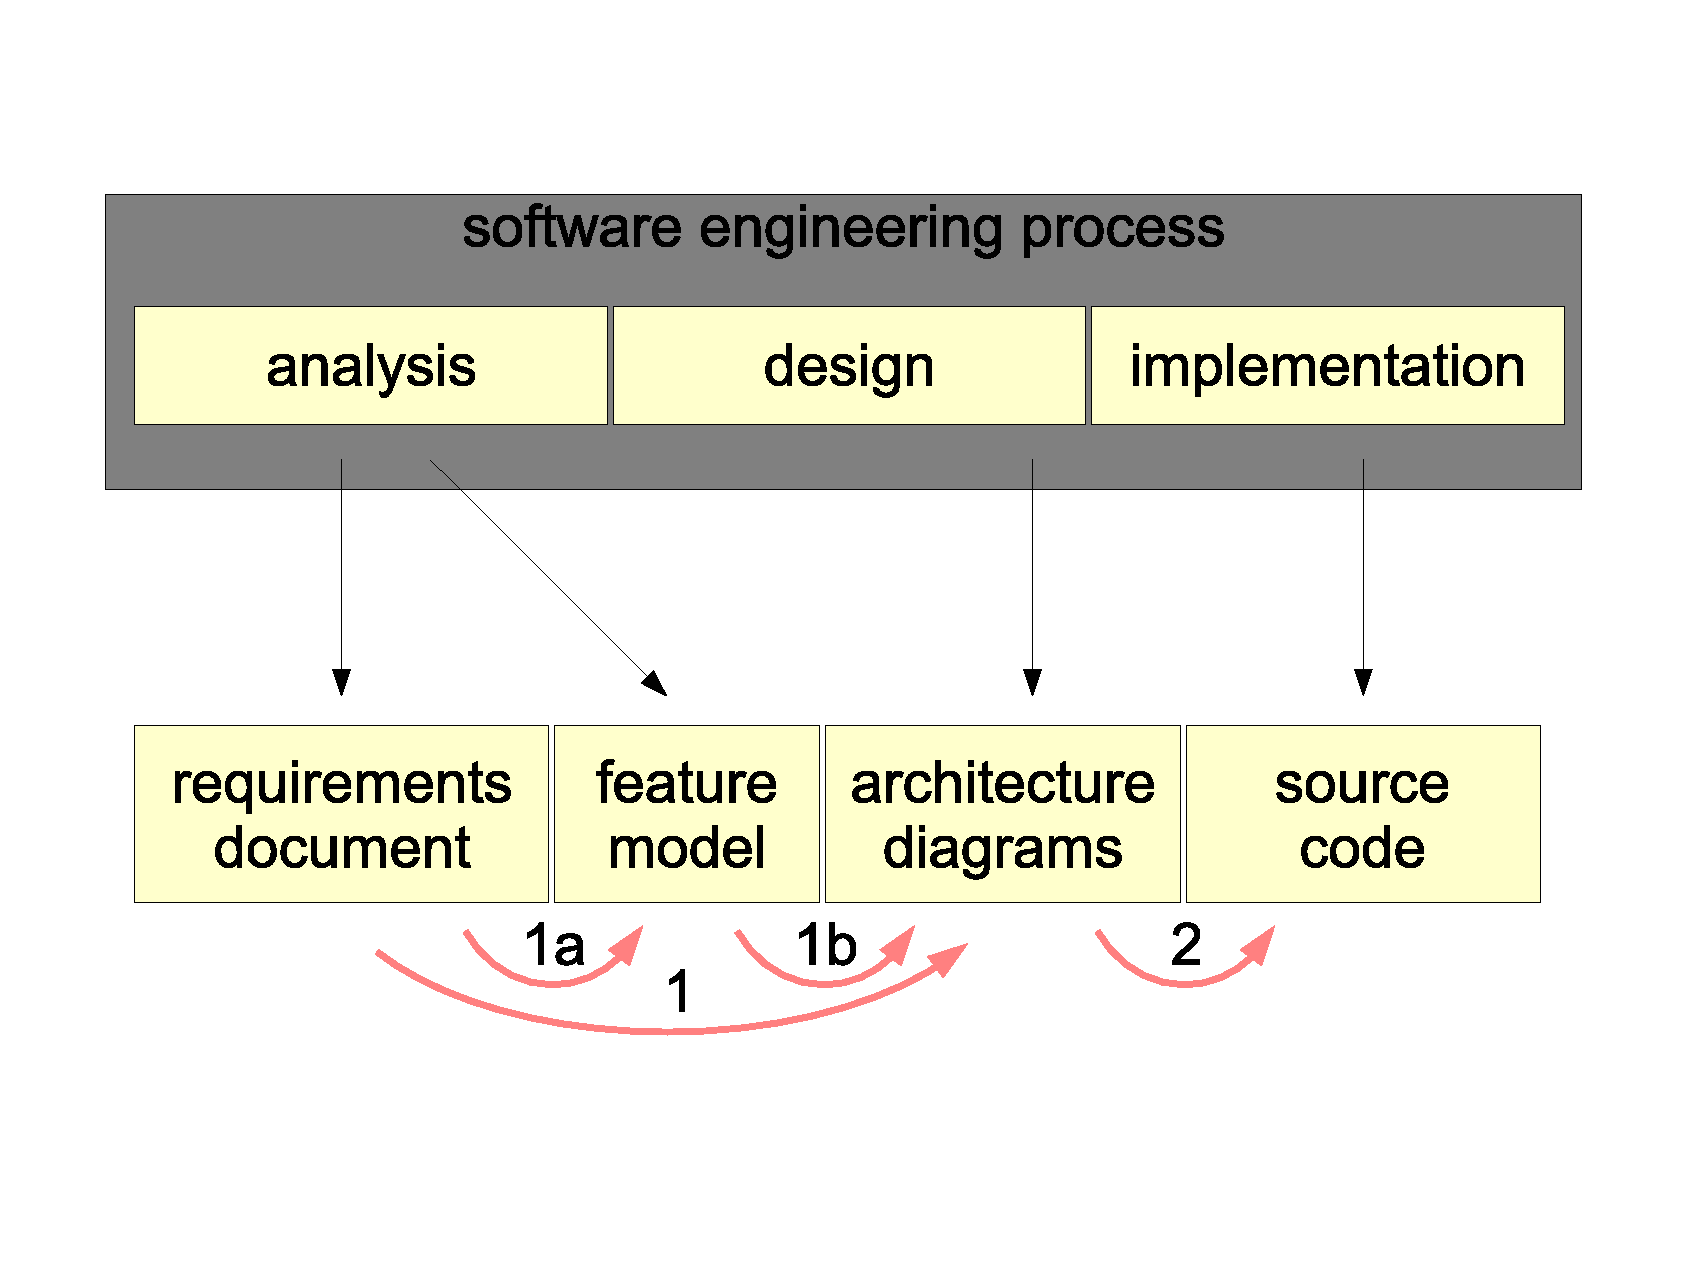
\includegraphics[scale=0.2]{vector/gaps.eps}
        \caption{Abstraction Gaps}
        \label{gaps_figure}
    \end{center}
\end{figure}

Different forms of SEP exist: \emph{Waterfall},\\ \emph{Iterative},
\emph{Extreme Programming} (XP) and \emph{Agile Programming}. But every
project, consciously or not, follows a SEP that sooner-or-later, in one form or
the other, goes through three common phases: \emph{Analysis}, \emph{Design} and
\emph{Implementation}. Each phase creates its own model of what is to be
abstracted in software and it is the differences in exactly these models that
often cause complications.

A previous article \cite{heller2004} mentioned the\\ \emph{Requirements Document},
\emph{Feature Model},\\ \emph{Architecture Diagrams} and \emph{Source Code} as
forms of knowledge abstraction. It also described the following abstraction
gaps (see figure \ref{gaps_figure}) that have to be crossed:

\begin{enumerate}
    \item[1a] Requirements Document -- Feature M.
    \item[1b] Feature Model -- Architecture Diagr.
    \item[2] Architecture Diagrams -- Source Code
\end{enumerate}

By improving the \emph{Traceability} between requirements and the architecture,
feature models (known from system family/ product line engineering) contribute
to minimising gap 1. Together with architecture diagrams, they ease
communication between stakeholders in the SEP, because of their human-readable
form and implementation-independence. But sooner-or-later, also these have to
be transferred into source code, by crossing gap 2.

Bridging or closing these abstraction gaps (sometimes called \emph{Semantic- or
Conceptual Gaps}) is also known as: \textit{achieving higher intentionality}
and remains an unsolved task for software engineering. One aim of the work
described in this article was to contribute to a possible solution, with focus
on \emph{reducing} gap 2, existing between a designed architecture and the
implemented code.

%
% $RCSfile: misleading_tiers.tex,v $
%
% Copyright (c) 2005-2006. Christian Heller. All rights reserved.
%
% Permission is granted to copy, distribute and/or modify this document
% under the terms of the GNU Free Documentation License, Version 1.1 or
% any later version published by the Free Software Foundation; with no
% Invariant Sections, with no Front-Cover Texts and with no Back-Cover
% Texts. A copy of the license is included in the section entitled
% "GNU Free Documentation License".
%
% http://www.cybop.net
% - Cybernetics Oriented Programming -
%
% http://www.resmedicinae.org
% - Information in Medicine -
%
% Version: $Revision: 1.1 $ $Date: 2006-01-03 08:21:45 $ $Author: christian $
% Authors: Christian Heller <christian.heller@tuxtax.de>
%

\subsection{Misleading Tiers}
\label{misleading_tiers_heading}

When distinguishing human- and technical systems, the kinds of
\emph{Communication} are:

\begin{itemize}
    \item[-] Human $\leftrightarrow$ Human
    \item[-] Human $\leftrightarrow$ Computer
    \item[-] Computer $\leftrightarrow$ Computer
\end{itemize}

Each of these relies on different techniques, transport mechanisms, languages
(protocols) and so on. But the general principle after which communication
works, is always the same -- no matter whether technical \emph{Computer}
systems or their biological prototype, the \emph{Human Being}, are considered:
Information is \emph{received}, \emph{stored}, \emph{processed} and \emph{sent}.
Despite these common characteristics, today's \emph{Information Technology}
(IT) environments \cite{hellerkunze} treat communication between a computer
system and a human being differently than that \emph{among} computer systems.

\begin{figure}[ht]
    \begin{center}
        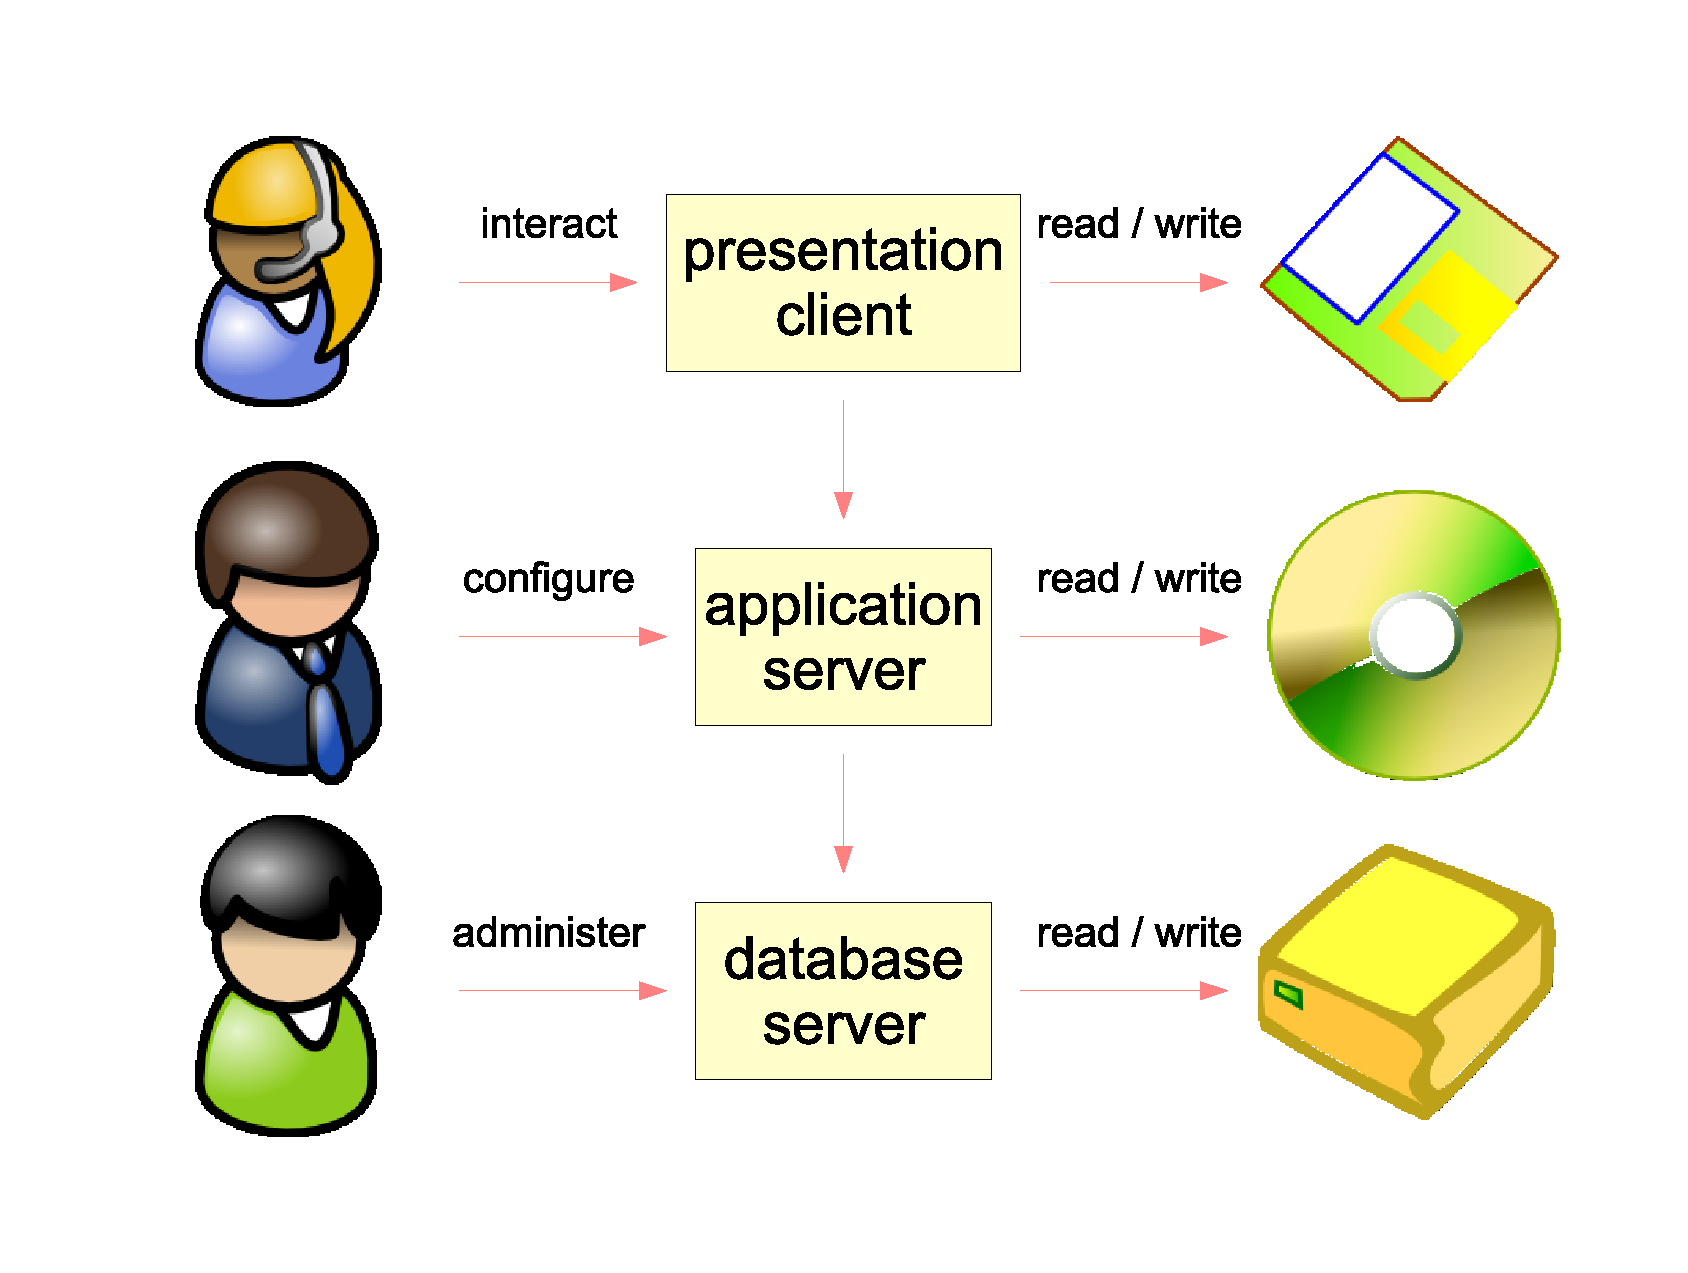
\includegraphics[scale=0.2]{vector/universal.eps}
        \caption{Universal Communication}
        \label{universal_figure}
    \end{center}
\end{figure}

Figure \ref{universal_figure} shows a three-tier environment: tier 1 represents
the \emph{Presentation Layer}; tier 2 stands for the \emph{Application Layer};
tier 3 is the \emph{Database (DB) Layer}. Typical synonyms are, in this order:
\emph{Frontend}, \emph{Business Logic} and \emph{Backend}. The tiers (layers)
serve two needs: connect different locations and share work load (\emph{Scaling}).
However, the split into tiers of that kind raises two illusions:

\begin{enumerate}
    \item \emph{Users only interact with clients}
    \item \emph{Persistent data are stored in DB only}
\end{enumerate}

Many IT architectures, or at least their illustrations, neglect the fact that
in reality \emph{all} systems need a \emph{User Interface} (UI), for at least
being administered by humans, and \emph{almost} all systems, even
\emph{Database Management Systems} (DBMS) themselves, store some of their
persistent data outside a database, for example locally available configuration
information. This is not necessarily a problem for the IT environment as such,
but it is for the internal architecture of software systems. Special solutions
have to deal with frontend (UI framework), business logic (domain patterns) and
backend (data mapping), and often additional mechanisms for local and remote
communication. The serious differences in these design solutions are one root
of well-known problems like multi- directional inter-dependencies between system
parts, that make software difficult to develop and hard to maintain.

One aim of the work described in this article was to investigate possibilities
for a \emph{unification} of communication paradigms, that is high-level design
paradigms rather than low-level protocols, in order to architect software in a
way that allows the computer system it runs on to communicate \emph{universally}.

%
% $RCSfile: modelling_mistakes.tex,v $
%
% Copyright (c) 2005-2006. Christian Heller. All rights reserved.
%
% Permission is granted to copy, distribute and/or modify this document
% under the terms of the GNU Free Documentation License, Version 1.1 or
% any later version published by the Free Software Foundation; with no
% Invariant Sections, with no Front-Cover Texts and with no Back-Cover
% Texts. A copy of the license is included in the section entitled
% "GNU Free Documentation License".
%
% http://www.cybop.net
% - Cybernetics Oriented Programming -
%
% http://www.resmedicinae.org
% - Information in Medicine -
%
% Version: $Revision: 1.1 $ $Date: 2006-01-03 08:21:45 $ $Author: christian $
% Authors: Christian Heller <christian.heller@tuxtax.de>
%

\subsection{Modelling Mistakes}
\label{modelling_mistakes_heading}

Most modern software is not written directly in a machine language but designed
in form of higher-level models instead. These allow to speed up application
development and help avoiding errors. \emph{Object Oriented Programming} (OOP),
for example, uses design concepts like the \emph{Class} owning \emph{Attributes}
and \emph{Methods}. Yet does this kind of modelling create abstractions that
reflect concepts of the real world completely and correctly?

\begin{figure}[ht]
    \begin{center}
        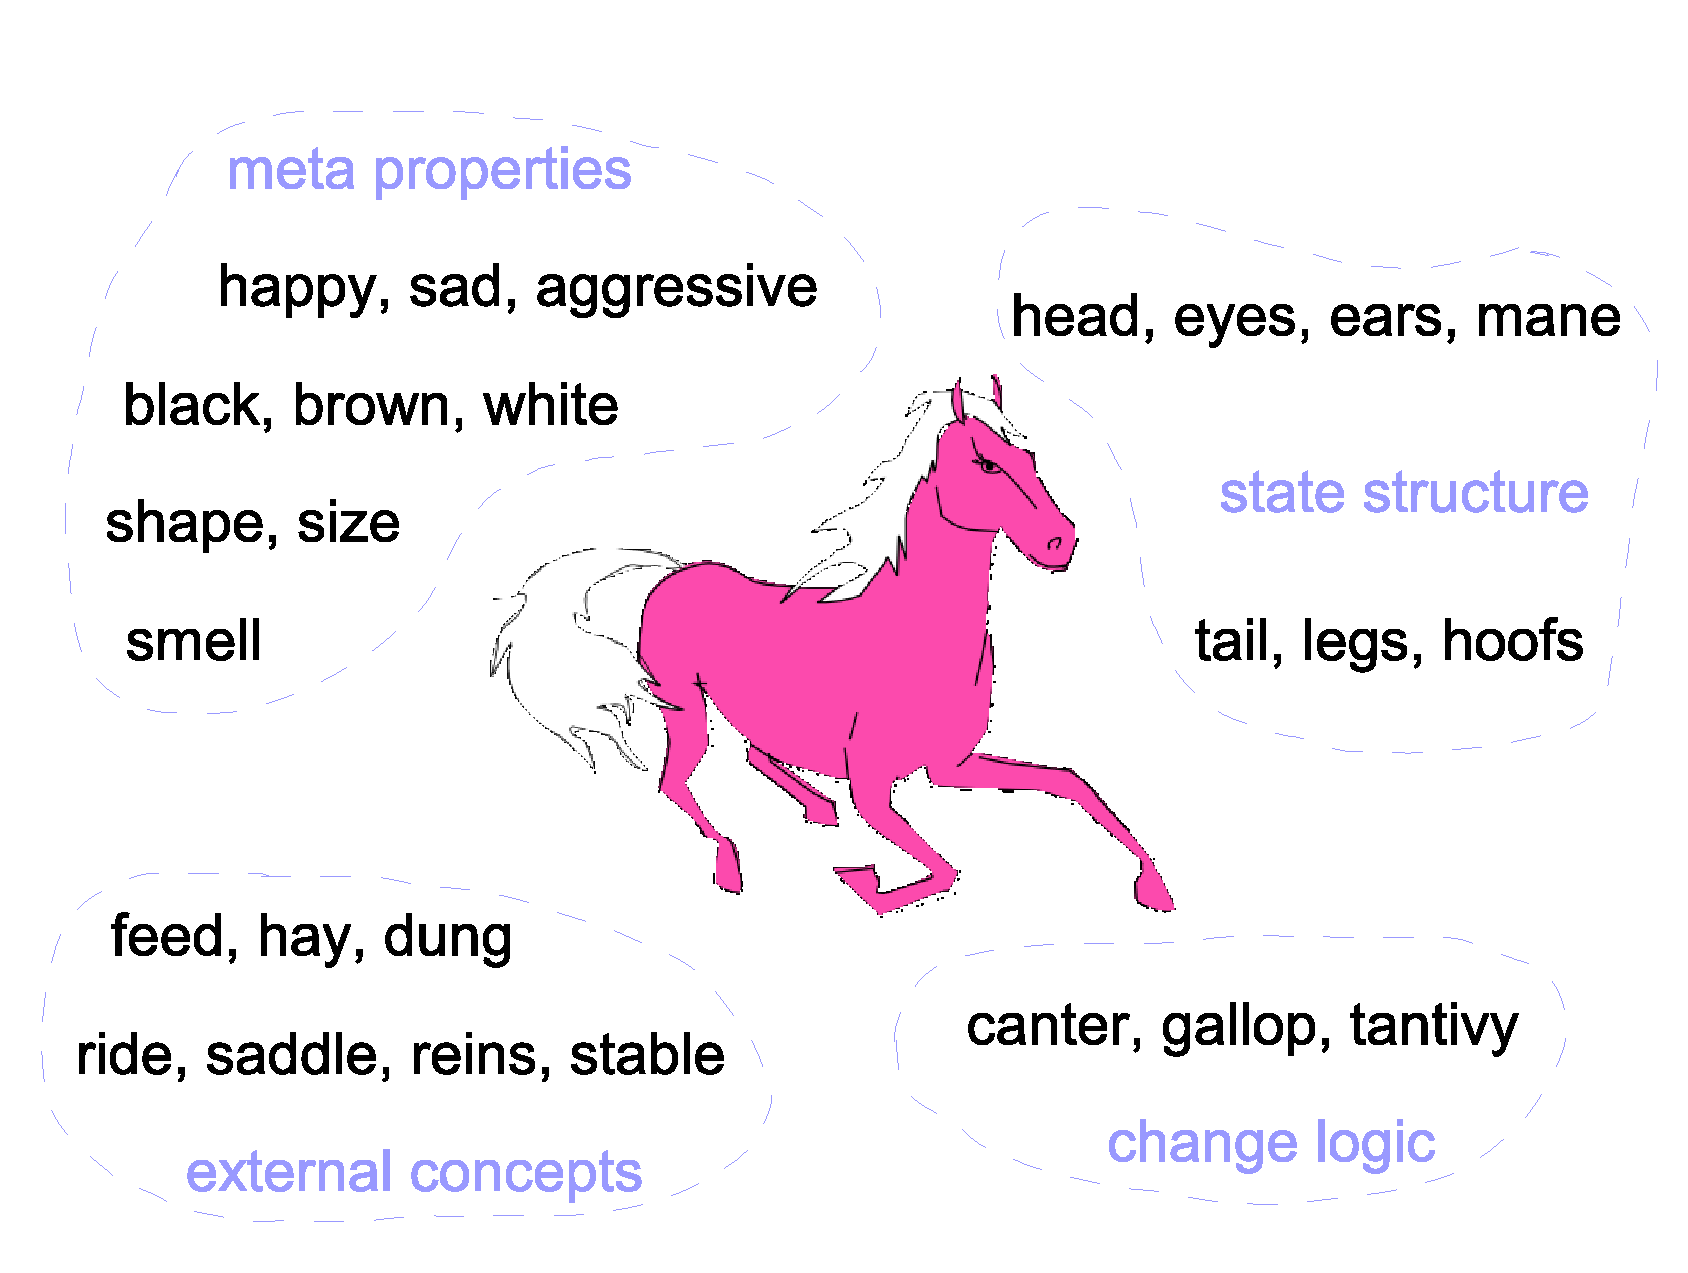
\includegraphics[scale=0.2]{vector/horse.eps}
        \caption{Concept of a Horse}
        \label{horse_figure}
    \end{center}
\end{figure}

The model of a \emph{Horse} shall serve as example to investigate this further.
Figure \ref{horse_figure} shows a number of terms commonly used to describe a
horse. Most importantly, there are structural observations describing the horse
as concept consisting of parts like \emph{Head}, \emph{Legs} or \emph{Hoofs}.
Secondly, there are properties like the horse's \emph{Colour}, \emph{Shape} or
\emph{Size}. Thirdly, there are terms describing a horse's actions like its
\emph{Movement} or \emph{Eating}, that change a horse's position and/ or state.
Finally, there are a number of terms like \emph{Hay} or \emph{Saddle}
associating concepts related to the horse.

One might suggest to model properties like the position, size or colour of a
horse's leg as \emph{Part} of that leg. In fact, this is how classical
programming approaches its solutions. In OOP, one would probably use a class
representing the leg and an attribute standing for the leg's colour. However,
when following the modelling principles of human thinking (see
\cite{heller2004}), this is \emph{not} correct!

It is true that in everyday language, one tends to say \textit{A horse leg
\emph{has a} colour.} Unfortunately, this leads to the wrong assumption that a
leg were made of a colour. But this is not the case. A leg does not
\emph{consist} of a colour in the hierarchical meaning of a whole consisting of
parts. The colour is rather property information \emph{about} the leg. It seems
there is no correct expression in natural (English) language stating the
property of something. The \emph{IS-A} verbalisation is used to express that
the leg belongs to a special category of items, for example: \textit{A leg is a
body element.} The \emph{HAS-A} formulation is used to express that a leg as
whole consists of smaller parts, for example: \textit{A leg has a knee and it
has a hoof.} But which formulation expresses a property? Well, perhaps it would
be best to say: \textit{A leg IS-OF a colour.}

The CYBOP knowledge schema described later in this article distinguishes
structural- from meta information. Actions (like the gallop of a horse) causing
change in the model or its environment are called \emph{Logic} in this work,
since they follow certain rules.


    \newpage{\pagestyle{empty}\cleardoublepage}
    %
% $RCSfile: definition.tex,v $
%
% Copyright (c) 2002-2007. Christian Heller. All rights reserved.
%
% Permission is granted to copy, distribute and/or modify this document
% under the terms of the GNU Free Documentation License, Version 1.1 or
% any later version published by the Free Software Foundation; with no
% Invariant Sections, with no Front-Cover Texts and with no Back-Cover
% Texts. A copy of the license is included in the section entitled
% "GNU Free Documentation License".
%
% http://www.cybop.net
% - Cybernetics Oriented Programming -
%
% Version: $Revision: 1.2 $ $Date: 2007-08-01 13:59:00 $ $Author: christian $
% Authors: Christian Heller <christian.heller@tuxtax.de>
%

\chapter{Definition}
\label{definition_heading}
\index{Definition}
\index{Whole-Part Hierarchy}
\index{Meta Data Hierarchy}
\index{Extensible Markup Language}
\index{XML}

This chapter defines the \emph{Syntax}, \emph{Vocabulary} and \emph{Semantics}
of the CYBOL language.

As already mentioned in chapter \ref{introduction_heading}, CYBOL is based upon
\emph{two} kinds of hierarchies. One of them is representing \emph{Whole-Part}
relations (such as a graphical window consisting of a menu bar) and the other
the \emph{Meta Data} which a whole keeps about its parts (such as the size or
colour of the menu bar). More details and the philosophical background are
described in \cite{cybopbook}. The syntax and semantics of CYBOL as new
language must be rich enough to express abstract knowledge models using this
kind of double hierarchy.

%
% $RCSfile: syntax.tex,v $
%
% Copyright (C) 2002-2008. Christian Heller.
%
% Permission is granted to copy, distribute and/or modify this document
% under the terms of the GNU Free Documentation License, Version 1.1 or
% any later version published by the Free Software Foundation; with no
% Invariant Sections, with no Front-Cover Texts and with no Back-Cover
% Texts. A copy of the license is included in the section entitled
% "GNU Free Documentation License".
%
% http://www.cybop.net
% - Cybernetics Oriented Programming -
%
% http://www.resmedicinae.org
% - Information in Medicine -
%
% Version: $Revision: 1.1 $ $Date: 2008-08-19 20:41:09 $ $Author: christian $
% Authors: Christian Heller <christian.heller@tuxtax.de>
%

\subsection{Syntax}
\label{syntax_heading}
\index{CYBOL Syntax}
\index{Syntax of a Language}
\index{Grammar of a Language}
\index{Extensible Markup Language}
\index{XML}
\index{XML Tag}
\index{XML Attribute}
\index{Discrimination}
\index{Composition}

Every language has a special \emph{Syntax}, that is a \emph{Grammar} with rules
for combining terms and symbols \cite{foldoc}. CYBOL could define its own
syntax or use an already existing one, of another language. Because of its
popularity, clear text representation, flexibility, extensibility and ease of
use, \emph{XML} was chosen to deliver the syntax for CYBOL.

To mention just two of the syntactical elements of XML, \emph{Tag} and
\emph{Attribute} are considered shortly here. Tags are special, arbitrary
keywords that have to be defined by the system working with an XML document.
Attributes keep additional information about the contents enclosed by two tags.
Two examples:

\begin{scriptsize}
    \begin{verbatim}
    <tag attribute="value">
        contents
    </tag>
    \end{verbatim}
\end{scriptsize}

\begin{scriptsize}
    \begin{verbatim}
    <tag attribute1="value" attribute2="contents"/>
    \end{verbatim}
\end{scriptsize}

An XML document carries a name and can such represent a \emph{Discrete Item},
as suggested by the principles of human thinking (section
\ref{human_thinking_heading}). Being a \emph{Compound}, it consists of parts --
and, it can link to other documents treated as its parts. That way, a whole
hierarchy can be formed. Tag attributes can keep additional information about
the linked parts. Most importantly, XML documents have a hierarchical structure
based on tags, which may be used to store meta information about a part.

Considering these properties of XML, it seems predestinated for formally
representing abstract models using the CYBOP concepts. CYBOL, finally, is XML
\emph{plus} a defined set of tags, attributes and values, used to structure and
link documents meaningfully.

%
% $RCSfile: vocabulary.tex,v $
%
% Copyright (c) 2001-2004. Christian Heller. All rights reserved.
%
% No copying, altering, distribution or any other actions concerning this
% document, except after explicit permission by the author!
% At some later point in time, this document is planned to be put under
% the GNU FDL license. For now, _everything_ is _restricted_ by the author.
%
% http://www.cybop.net
% - Cybernetics Oriented Programming -
%
% http://www.resmedicinae.org
% - Information in Medicine -
%
% @author Christian Heller <christian.heller@tuxtax.de>
%

\subsection{Vocabulary}
\label{vocabulary_heading}

XML allows to define and exchange the whole vocabulary of a language. It offers
two ways in which a list of legal elements can be defined: The traditional
\emph{Document Type Definition} (DTD) and the more modern \emph{XML Schema
Definition} (XSD). Besides the vocabulary, DTD and XSD define the structure of
an XML document and allow to typify, constrain and validate items. The CYBOL DTD
and XSD can be found at \cite{cybop}.

%
% $RCSfile: semantics.tex,v $
%
% Copyright (c) 2002-2007. Christian Heller. All rights reserved.
%
% Permission is granted to copy, distribute and/or modify this document
% under the terms of the GNU Free Documentation License, Version 1.1 or
% any later version published by the Free Software Foundation; with no
% Invariant Sections, with no Front-Cover Texts and with no Back-Cover
% Texts. A copy of the license is included in the section entitled
% "GNU Free Documentation License".
%
% http://www.cybop.net
% - Cybernetics Oriented Programming -
%
% Version: $Revision: 1.1 $ $Date: 2007-08-01 13:59:00 $ $Author: christian $
% Authors: Christian Heller <christian.heller@tuxtax.de>
%

\section{Semantics}
\label{semantics_heading}
\index{Semantics}
\index{State Knowledge Modelling}
\index{Logic Knowledge Modelling}
\index{Extensible Markup Language}
\index{XML}
\index{XML Tag}
\index{XML Attribute}

The meaning expressed by terms and sentences is their \emph{Semantics}
\cite{duden}.

CYBOL files can be used to model \emph{State Knowledge} (like a graphical
window or a person's address) and \emph{Logic Knowledge} (like an operation or
algorithm or workflow) \cite{cybopbook}. In both cases, the \emph{same} syntax
(document structure) with \emph{identical} vocabulary (XML tags and -attributes)
is applied. It is the attribute \emph{Values} that make a difference in meaning.

The double hierarchy mentioned before is realised in CYBOL knowledge templates
by using XML \emph{Attributes} for representing the whole-part hierarchy, and
XML \emph{Tags} for representing the additional meta data that a whole model
keeps about its part models.

%
% $RCSfile: attributes.tex,v $
%
% Copyright (C) 2002-2008. Christian Heller.
%
% Permission is granted to copy, distribute and/or modify this document
% under the terms of the GNU Free Documentation License, Version 1.1 or
% any later version published by the Free Software Foundation; with no
% Invariant Sections, with no Front-Cover Texts and with no Back-Cover
% Texts. A copy of the license is included in the section entitled
% "GNU Free Documentation License".
%
% http://www.cybop.net
% - Cybernetics Oriented Programming -
%
% http://www.resmedicinae.org
% - Information in Medicine -
%
% Version: $Revision: 1.1 $ $Date: 2008-08-19 20:41:05 $ $Author: christian $
% Authors: Christian Heller <christian.heller@tuxtax.de>
%

\subsubsection{Attributes}
\label{attributes_heading}
\index{CYBOL Attributes}
\index{CYBOL 'name' Attribute}
\index{CYBOL 'channel' Attribute}
\index{CYBOL 'abstraction' Attribute}
\index{CYBOL 'model' Attribute}

Normally, an XML \emph{Attribute} keeps meta information about the contents of
an XML \emph{Tag}. In CYBOL, however, three attributes keep meta information
about a fourth attribute. The attributes, altogether, are:

\begin{itemize}
    \item[-] name
    \item[-] channel
    \item[-] abstraction
    \item[-] model
\end{itemize}

The attribute of greatest interest is \emph{model}. It contains a model either
directly, or a path to one. The \emph{channel} attribute indicates whether the
\emph{model} attribute's value is to be read from:

\begin{itemize}
    \item[-] inline
    \item[-] file
    \item[-] ftp
    \item[-] http
\end{itemize}

The \emph{abstraction} attribute specifies how to interpret the model pointed
to by the \emph{model} attribute's value. A model may be given in formats like
for example:

\newpage

\begin{itemize}
    \item[-] cybol (a state- or logic compound model encoded in CYBOL format)
    \item[-] operation (a primitive logic model)
    \item[-] string
    \item[-] double
    \item[-] integer
    \item[-] boolean
\end{itemize}

The \emph{name} attribute, finally, provides the referenced model with a unique
identifier.

While the interpretation of the \emph{model} attribute's value depends on the
\emph{channel-} and \emph{abstraction} attributes, the other three attributes
(\emph{name}, \emph{channel}, \emph{abstraction}) themselves always get
interpreted as character string.

%
% $RCSfile: tags.tex,v $
%
% Copyright (C) 2002-2008. Christian Heller.
%
% Permission is granted to copy, distribute and/or modify this document
% under the terms of the GNU Free Documentation License, Version 1.1 or
% any later version published by the Free Software Foundation; with no
% Invariant Sections, with no Front-Cover Texts and with no Back-Cover
% Texts. A copy of the license is included in the section entitled
% "GNU Free Documentation License".
%
% http://www.cybop.net
% - Cybernetics Oriented Programming -
%
% http://www.resmedicinae.org
% - Information in Medicine -
%
% Version: $Revision: 1.1 $ $Date: 2008-08-19 20:41:09 $ $Author: christian $
% Authors: Christian Heller <christian.heller@tuxtax.de>
%

\subsubsection{Tags}
\label{tags_heading}
\index{CYBOL Tags}
\index{CYBOL 'model' Tag}
\index{CYBOL 'part' Tag}
\index{CYBOL 'property' Tag}
\index{CYBOL 'constraint' Tag}

There are many kinds of meta information besides the above-mentioned
attributes, that may be known about a model. These are given in special XML
tags called \emph{property} and \emph{constraint}. As defined in section
\ref{vocabulary_heading}, a CYBOL knowledge template may use four kinds of XML
tags:

\begin{itemize}
    \item[-] model
    \item[-] part
    \item[-] property
    \item[-] constraint
\end{itemize}

The \emph{model} tag appears just once. It is the root node which makes a CYBOL
knowledge template a valid XML document.

Of actual interest are the \emph{part} tags. They identify the models that the
\emph{whole} model described by the CYBOL knowledge template consists of.

A \emph{whole} model may know a lot more about its \emph{part} models, than is
given by a part model's XML attributes. A spatial state model may know about
the \emph{position} and \emph{size} of its parts, in space. A temporal model
(such as a workflow) may have to know about the \emph{position} of its parts in
time, in order to be able to execute them in the correct order. Further, the
temporal model needs to know about the \emph{input/output} (i/o) state models
which are to be manipulated by the corresponding logic operation (part model).
The number of parts within a whole (compound) model may be limited. And so on.
These additional information are provided by \emph{property} tags whose number
is conceptually unlimited.

Not only parts need additional meta information; properties may need such
information, too. The position or size as properties of a part may have to be
constrained to certain values, such as a \emph{minimum} or \emph{maximum}. The
values of the \emph{colour} property of a part model may have to be chosen out
of a pre-defined set called \emph{choice}. Information of that kind are stated
in \emph{constraint} tags.

Since the number of possible meta information implementable in CYBOL is already
quite large and steadily growing, as the development continues, this section
cannot list them all. At a future point in time, a more-or-less complete CYBOL
specification document may be found at the CYBOP project's website \cite{cybop}.

%
% $RCSfile: tag_attribute_swapping.tex,v $
%
% Copyright (C) 2002-2008. Christian Heller.
%
% Permission is granted to copy, distribute and/or modify this document
% under the terms of the GNU Free Documentation License, Version 1.1 or
% any later version published by the Free Software Foundation; with no
% Invariant Sections, with no Front-Cover Texts and with no Back-Cover
% Texts. A copy of the license is included in the section entitled
% "GNU Free Documentation License".
%
% http://www.cybop.net
% - Cybernetics Oriented Programming -
%
% http://www.resmedicinae.org
% - Information in Medicine -
%
% Version: $Revision: 1.1 $ $Date: 2008-08-19 20:41:09 $ $Author: christian $
% Authors: Christian Heller <christian.heller@tuxtax.de>
%

\subsection{Tag-Attribute Swapping}
\label{tag_attribute_swapping_heading}
\index{CYBOL Tag-Attribute Swapping}

CYBOL swaps the meaning attributes and tags traditionally have in XML
documents, where tags represent elements that may be nested infinitely and
attributes hold additional (meta) information about a tag. Following an example
of how CYBOL might have looked that way:

\begin{scriptsize}
    \begin{verbatim}
<model>
    <part>
        <name="title"/>
        <channel="inline"/>
        <abstraction="character"/>
        <model="Res Medicinae"/>
    </part>
    <part layout="compass" position="north">
        <name="menu_bar"/>
        <channel="file"/>
        <abstraction="cybol"/>
        <model="gui/menu_bar.cybol"/>
    </part>
</model>
    \end{verbatim}
\end{scriptsize}

The current final specification of CYBOL, on the contrary, uses attributes to
define a nested element (part) and tags to give properties (meta information)
about such a nested element, in the following way:

\begin{scriptsize}
    \begin{verbatim}
<model>
    <part name="title" channel="inline" abstraction="character" model="Res Medicinae"/>
    <part name="menu_bar" channel="file" abstraction="cybol" model="gui/menu_bar.cybol">
        <property name="layout" channel="inline" abstraction="character" model="compass"/>
        <property name="position" channel="inline" abstraction="character" model="north"/>
    </part>
</model>
    \end{verbatim}
\end{scriptsize}

This is because:

\begin{enumerate}
    \item the number of attributes specifying a part in CYBOL is fixed, whereas
        the number of tags specifying a property of a part is not, and the
        number of XML tags is easier extensible than that of attributes;
    \item that way it is also possible to specify a part without any properties
        in just one CYBOL code line, while otherwise four tags would always
        have to be given;
    \item not only a part may be nested (consist of smaller parts), but also a
        property may be (for example a position consisting of three coordinates
        given as parts), which necessitates the four standard attributes to be
        given for properties and constraints as well.
\end{enumerate}



    \newpage{\pagestyle{empty}\cleardoublepage}
    \input{names}
    \newpage{\pagestyle{empty}\cleardoublepage}
    \input{channels}
    \newpage{\pagestyle{empty}\cleardoublepage}
    \input{abstractions}
    \newpage{\pagestyle{empty}\cleardoublepage}
    \input{state_models}
    \newpage{\pagestyle{empty}\cleardoublepage}
    %
% $RCSfile: logic_models.tex,v $
%
% Copyright (c) 2002-2007. Christian Heller. All rights reserved.
%
% Permission is granted to copy, distribute and/or modify this document
% under the terms of the GNU Free Documentation License, Version 1.1 or
% any later version published by the Free Software Foundation; with no
% Invariant Sections, with no Front-Cover Texts and with no Back-Cover
% Texts. A copy of the license is included in the section entitled
% "GNU Free Documentation License".
%
% http://www.cybop.net
% - Cybernetics Oriented Programming -
%
% Version: $Revision: 1.2 $ $Date: 2007-08-01 13:59:00 $ $Author: christian $
% Authors: Christian Heller <christian.heller@tuxtax.de>
%

\chapter{Logic Models}
\label{logic_models_heading}
\index{Logic Models}

\input{bit_manipulation}
%
% $RCSfile: boolean_logic.tex,v $
%
% Copyright (C) 2002-2008. Christian Heller.
%
% Permission is granted to copy, distribute and/or modify this document
% under the terms of the GNU Free Documentation License, Version 1.1 or
% any later version published by the Free Software Foundation; with no
% Invariant Sections, with no Front-Cover Texts and with no Back-Cover
% Texts. A copy of the license is included in the section entitled
% "GNU Free Documentation License".
%
% http://www.cybop.net
% - Cybernetics Oriented Programming -
%
% http://www.resmedicinae.org
% - Information in Medicine -
%
% Version: $Revision: 1.1 $ $Date: 2008-08-19 20:41:05 $ $Author: christian $
% Authors: Christian Heller <christian.heller@tuxtax.de>
%

\subsubsection{Boolean Logic}
\label{boolean_logic_heading}
\index{Boolean Logic}
\index{Boolean Algebra}
\index{Union Operation}
\index{Intersection Operation}
\index{Complement Operation}
\index{AND Operation}
\index{OR Operation}
\index{NOT Operation}

Almost twohundred years after Leibnitz completed his binary arithmetic, George
Boole (1815-1864) took on those ideas and formed his \emph{Boolean Algebra},
described in \emph{An Investigation into the Laws of Thought, on which are
founded the Mathematical Theories of Logic and Probabilities} (1854). The St.
Andrew's website \cite{standrews} states:

\begin{quote}
    Boole approached logic in a new way reducing it to a simple algebra,
    incorporating logic into mathematics. He pointed out the analogy between
    algebraic symbols and those that represent logical forms. It began the
    algebra of logic called Boolean algebra which now finds application in
    computer construction, switching circuits etc.
\end{quote}

The same site describes Boole's theory as: \textit{a system of symbolic logic}
and: \textit{an algebra in which the binary operations are chosen to model the
union and intersection operations in Set Theory. For any set A, the subsets of
A form a Boolean algebra under the operations of union, intersection and
complement.}

Boolean postulates and laws \cite{belton} are based on three operations:
\emph{AND}, \emph{OR} and \emph{NOT}. Every Boolean algebra can be built up by
combining simple Boolean algebra, with its elements \emph{0} and \emph{1}.
These definitions make it possible to express and translate complex knowledge.
Sowa \cite{sowa} writes: \textit{Yet logic is all there is: every programming
language, specification language and requirements definition language can be
defined in logic; and nothing less can meet the requirements for a complete
definition system.}

\input{program_flow}
%
% $RCSfile: comparison.tex,v $
%
% Copyright (c) 2002-2007. Christian Heller. All rights reserved.
%
% Permission is granted to copy, distribute and/or modify this document
% under the terms of the GNU Free Documentation License, Version 1.1 or
% any later version published by the Free Software Foundation; with no
% Invariant Sections, with no Front-Cover Texts and with no Back-Cover
% Texts. A copy of the license is included in the section entitled
% "GNU Free Documentation License".
%
% http://www.cybop.net
% - Cybernetics Oriented Programming -
%
% Version: $Revision: 1.1 $ $Date: 2007-07-17 20:02:36 $ $Author: christian $
% Authors: Christian Heller <christian.heller@tuxtax.de>
%

\section{Comparison}
\label{comparison_heading}
\index{Comparison}

%
% $RCSfile: compare.tex,v $
%
% Copyright (c) 2002-2007. Christian Heller. All rights reserved.
%
% Permission is granted to copy, distribute and/or modify this document
% under the terms of the GNU Free Documentation License, Version 1.1 or
% any later version published by the Free Software Foundation; with no
% Invariant Sections, with no Front-Cover Texts and with no Back-Cover
% Texts. A copy of the license is included in the section entitled
% "GNU Free Documentation License".
%
% http://www.cybop.net
% - Cybernetics Oriented Programming -
%
% Version: $Revision: 1.1 $ $Date: 2007-07-17 20:02:36 $ $Author: christian $
% Authors: Christian Heller <christian.heller@tuxtax.de>
%

\subsection{Compare}
\label{compare_heading}
\index{Compare}

This operation compares two given operands.

\subsubsection{Comparison Property}

\emph{required}

name=\texttt{'comparison'}\\
abstraction=\texttt{'character'}\\
model=\texttt{'equal' \vline\ 'smaller' \vline\ 'greater' \vline\ 'smaller\_or\_equal' \vline\ 'greater\_or\_equal'}

This is the kind of comparison to be applied.

\subsubsection{Left Side Property}

\emph{required}

name=\texttt{'left\_side'}\\
abstraction=\texttt{'boolean' \vline\ 'integer' \vline\ 'float' \vline\ 'character' \vline\ 'knowledge' \vline\ 'encapsulated'}\\
model=\texttt{value or knowledge model}

This is the left side value of the comparison.

\subsubsection{Right Side Property}

\emph{required}

name=\texttt{'right\_side'}\\
abstraction=\texttt{'boolean' \vline\ 'integer' \vline\ 'float' \vline\ 'character' \vline\ 'knowledge' \vline\ 'encapsulated'}\\
model=\texttt{value or knowledge model}

This is the right side value of the comparison.

\subsubsection{Result Property}

\emph{required}

name=\texttt{'result'}\\
abstraction=\texttt{'boolean' \vline\ 'knowledge' \vline\ 'encapsulated'}\\
model=\texttt{result knowledge model}

This is the knowledge model in which the comparison result is stored.

\subsubsection{Selection Property}

\emph{optional}, only if comparing values of abstraction "character"

name=\texttt{'selection'}\\
abstraction=\texttt{'character'}\\
model=\texttt{'full' \vline\ 'prefix' \vline\ 'suffix' \vline\ 'part'}

This property selects which part of two string values shall be compared.


\input{arithmetic}
\input{memory_management}
%
% $RCSfile: lifecycle_management.tex,v $
%
% Copyright (C) 2002-2008. Christian Heller.
%
% Permission is granted to copy, distribute and/or modify this document
% under the terms of the GNU Free Documentation License, Version 1.1 or
% any later version published by the Free Software Foundation; with no
% Invariant Sections, with no Front-Cover Texts and with no Back-Cover
% Texts. A copy of the license is included in the section entitled
% "GNU Free Documentation License".
%
% http://www.cybop.net
% - Cybernetics Oriented Programming -
%
% http://www.resmedicinae.org
% - Information in Medicine -
%
% Version: $Revision: 1.1 $ $Date: 2008-08-19 20:41:07 $ $Author: christian $
% Authors: Christian Heller <christian.heller@tuxtax.de>
%

\subsection{Lifecycle Management}
\label{lifecycle_management_heading}
\index{CYBOI Lifecycle Management}

To the startup routine belong the creation of the three containers: knowledge
memory, signal memory and internals memory, and the creation of a startup model
which is placed as first signal into the signal memory. Additional meta
information given are the signal's model, its kind of abstraction and priority.

Typical synonyms for \emph{Signal} are \emph{Event} or \emph{Action} -- and
even an \emph{Operating System} (OS) \emph{Interrupt} is some form of signal,
only on a lower system level, closer to hardware. In CYBOI, a signal is simply
a reference to a logic model, which may be either a composed algorithm, or a
primitive operation.

With the startup signal being placed in the signal memory, the system enters
the \emph{check} procedure (\emph{checker} module). On shutdown, the system
runs through similar procedures in opposite direction, only that then startup
signal, memories and global variables are destroyed.

%
% $RCSfile: communication.tex,v $
%
% Copyright (C) 2002-2008. Christian Heller.
%
% Permission is granted to copy, distribute and/or modify this document
% under the terms of the GNU Free Documentation License, Version 1.1 or
% any later version published by the Free Software Foundation; with no
% Invariant Sections, with no Front-Cover Texts and with no Back-Cover
% Texts. A copy of the license is included in the section entitled
% "GNU Free Documentation License".
%
% http://www.cybop.net
% - Cybernetics Oriented Programming -
%
% http://www.resmedicinae.org
% - Information in Medicine -
%
% Version: $Revision: 1.1 $ $Date: 2008-08-19 20:41:05 $ $Author: christian $
% Authors: Christian Heller <christian.heller@tuxtax.de>
%

\subsection{Communication}
\label{communication_heading}
\index{Communication}
\index{Information Processing}

As described in the previous sections, humans have sensoric and motoric organs
responsible for information input and output. In between input and output, the
information is processed by the brain that contains a specific abstract model
of the surrounding real world. The human brain consists of several regions
(section \ref{brain_regions_heading}), each being responsible for a special
task, such as the optical region for seeing or the cerebral cortex for actual
information processing which possibly leads to awareness. Depending on which
medium, organ and language is used, systems may communicate across different
channels.

%
% $RCSfile: transient.tex,v $
%
% Copyright (C) 2002-2008. Christian Heller.
%
% Permission is granted to copy, distribute and/or modify this document
% under the terms of the GNU Free Documentation License, Version 1.1 or
% any later version published by the Free Software Foundation; with no
% Invariant Sections, with no Front-Cover Texts and with no Back-Cover
% Texts. A copy of the license is included in the section entitled
% "GNU Free Documentation License".
%
% http://www.cybop.net
% - Cybernetics Oriented Programming -
%
% http://www.resmedicinae.org
% - Information in Medicine -
%
% Version: $Revision: 1.1 $ $Date: 2008-08-19 20:41:09 $ $Author: christian $
% Authors: Christian Heller <christian.heller@tuxtax.de>
%

\subsubsection{Transient}
\label{transient_heading}
\index{Transient Communication}
\index{Direct Communication}
\index{Assembler}
\index{Mapper}
\index{Translator}
\index{Signal Processing}

Valentin Turchin \cite{turchin} writes:

\begin{quote}
    Sensations are produced by our sense organs. Perceptions are formed and used
    within the brain. Conceptions are created by ourselves while we create new,
    linguistic, models of the world.
    The triad: Sensation, Perception, Conception seems close in meaning to Kant's
    usage of these terms. We leave it to the reader, though, to judge on it.
\end{quote}

The following example demonstrates a typical information processing procedure.
Its sequential flow is illustrated in figure \ref{handling_figure} which uses
technical names, instead of biological ones. These can be found again in the
explaining text, enclosed in parentheses. The terms \emph{Assembler} and
\emph{Mapper} are converted and merged into the term \emph{Translator}.

\begin{figure}[ht]
    \begin{center}
        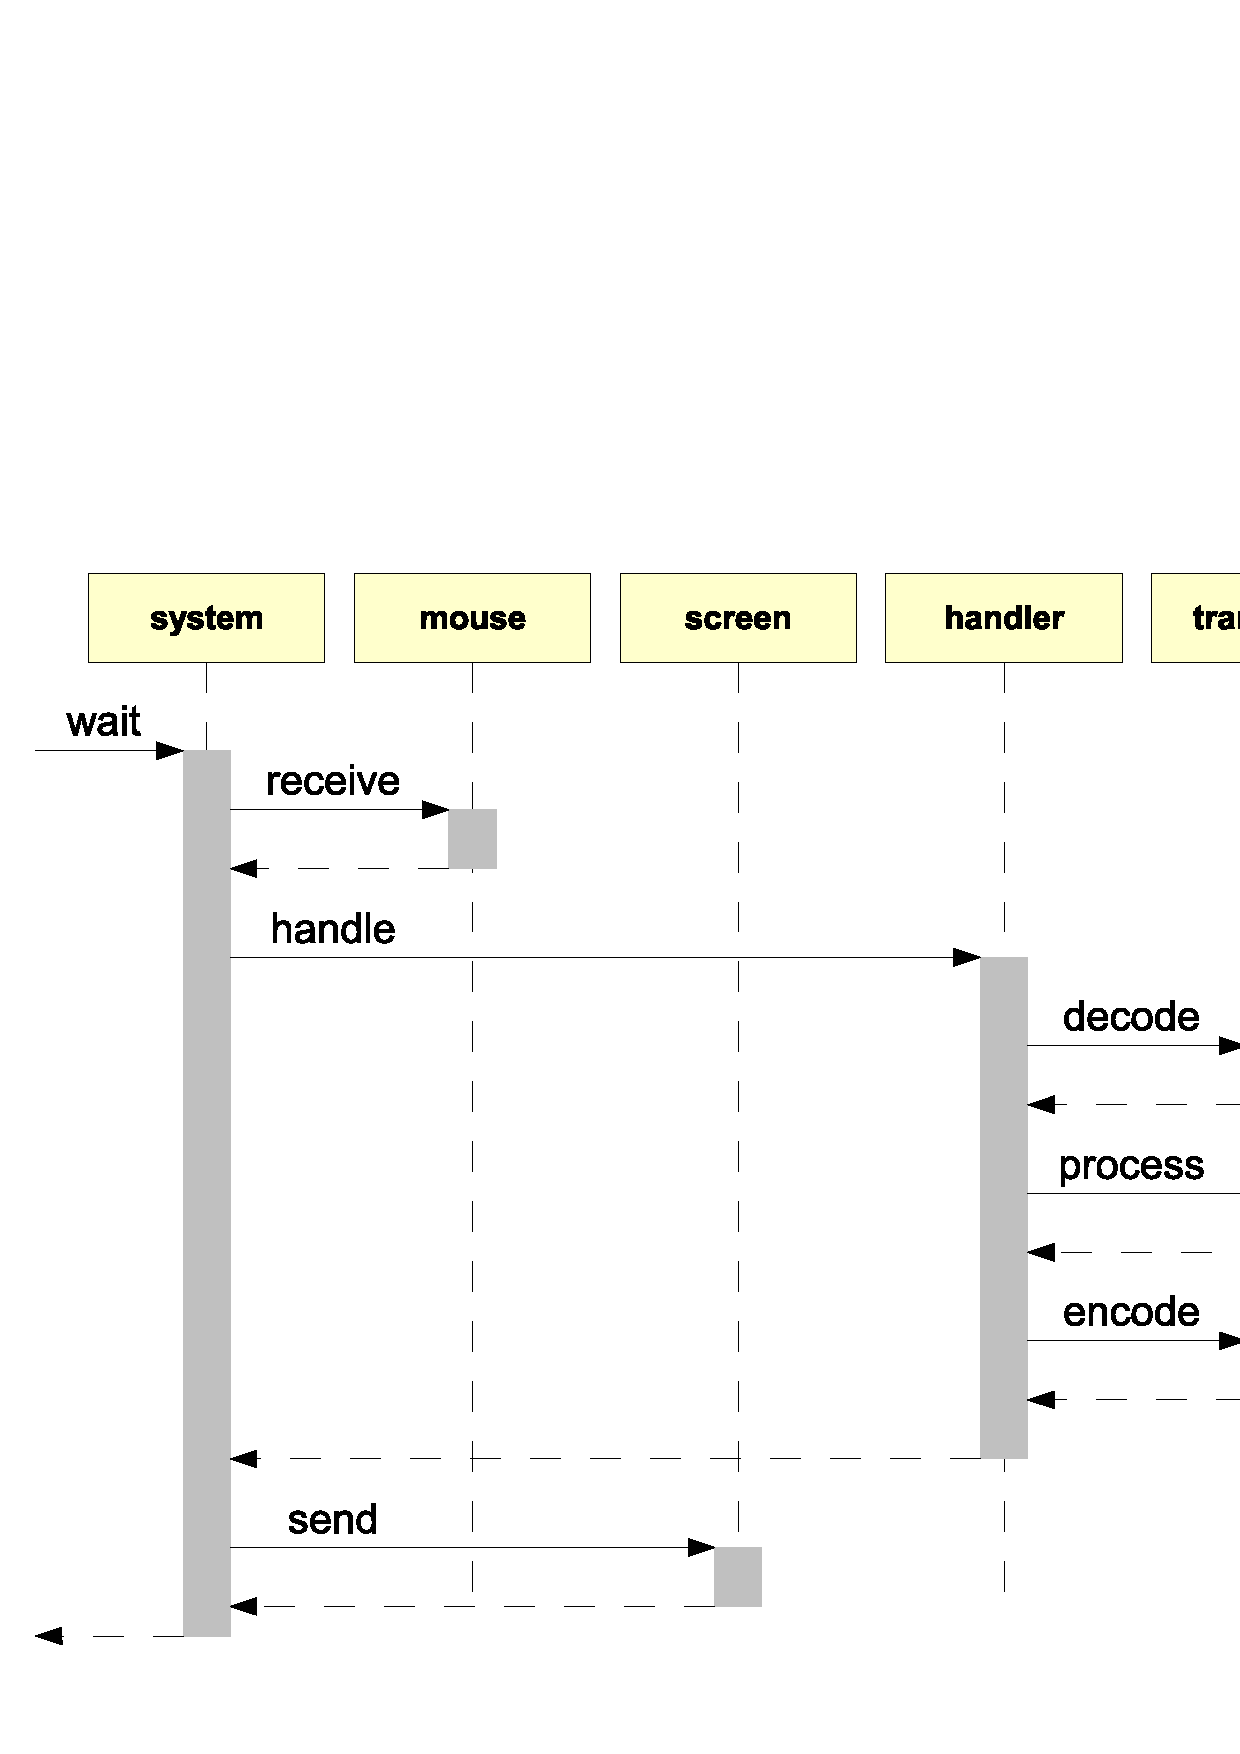
\includegraphics[scale=0.3,angle=-90]{graphic/handling.pdf}
        \caption{Signal Processing as UML Sequence Diagram}
        \label{handling_figure}
    \end{center}
\end{figure}

One human being (\emph{System}) wants to send a message to another. It decides
for an acoustical message (\emph{Signal}), formulates a sentence and talks. The
other human being, waiting for signals (\emph{wait}), receives the message
across its ear organ (\emph{Microphone}, \emph{Keyboard}, \emph{Mouse}). The
message is then forwarded to the receiver's brain (\emph{Handler}), where a
special region responsible for acoustics (\emph{Translator}) translates
(\emph{decode}) the data (\emph{Data Transfer Model}) contained in the message
and sorts them into the human's abstract model of the surrounding real world
(\emph{Domain Model}). Processing of the message happens in the cerebral cortex
of the brain (\emph{Processor}). If the addressed listener wants to send an
answer message (\emph{Signal}), it may do so by triggering a muscle reaction.
For this to happen, the motoric brain region (\emph{Translator}) needs to
translate (\emph{encode}) model data (\emph{Domain Model}) into a special
transfer model (\emph{User Interface Model}), for the answer. Finally, the
answer message (\emph{Signal}) will be sent as muscle action (data display on
\emph{Monitor}).

If a communication partner does not, or only partly receives a message, the
missing information is lost, unless the sender repeats it once more. The reason
is that the transport mediums (light, air) do not steadily contain the
information; the sent information is transient. Therefore, the whole process
described above can be called \emph{Transient Communication}.

%
% $RCSfile: persistent.tex,v $
%
% Copyright (C) 2002-2008. Christian Heller.
%
% Permission is granted to copy, distribute and/or modify this document
% under the terms of the GNU Free Documentation License, Version 1.1 or
% any later version published by the Free Software Foundation; with no
% Invariant Sections, with no Front-Cover Texts and with no Back-Cover
% Texts. A copy of the license is included in the section entitled
% "GNU Free Documentation License".
%
% http://www.cybop.net
% - Cybernetics Oriented Programming -
%
% http://www.resmedicinae.org
% - Information in Medicine -
%
% Version: $Revision: 1.1 $ $Date: 2008-08-19 20:41:08 $ $Author: christian $
% Authors: Christian Heller <christian.heller@tuxtax.de>
%

\subsubsection{Persistent}
\label{persistent_heading}
\index{Persistent Communication}
\index{Mediums for Knowledge Storage}
\index{Indirect Communication}
\index{Knowledge Carrier}
\index{Hard Disk Drive}
\index{HDD}
\index{Random Access Memory}
\index{RAM}

One great advantage of human beings is to be able to help each other, to
cooperate in order to reach a common aim, to form a society which is to fill
exactly these aims. Main tasks of a \emph{State} as one form of organisation of
society are: \emph{Security}, \emph{Education}, \emph{Social Welfare}. While
all of them depend upon \emph{Politics}, there is an additional factor playing
an increasingly important role: the \emph{Availability of Knowledge}. Knowledge
cannot only be exchanged between current citizens of earth; fortunately, it can
be forwarded over \emph{Generations}.

For this to become possible, mankind had to make use of different mediums for
external storage, such as: \emph{Rock Painting}, \emph{Stone Tablet},
\emph{Papyrus Roll}, \emph{Paper Book}, \emph{Chemical Film},
\emph{Electronic File}. It also had to invent technologies for the
dissemination of knowledge: \emph{Monks' copying by hand}, \emph{Library},
\emph{Printing}, \emph{Radio and TV}, \emph{Internet}. The following example
does therefore not deal with \emph{direct} inter-systems communication, but
rather its \emph{indirect} counterpart -- the interaction between a system and
mediums in its environment. Of course, that environment could be treated as
system, too; but for reasons of simplification it is not here.

One human being (\emph{System}) wants to send a message to another, which is
not near the same location, but at some remote place. The sender has to decide
for a persistent message, and to choose a non-transient medium to store that
message. He takes a piece of paper, writes down or paints some information and
finally sends that paper as letter by (snail) mail. Paper and letter act as
\emph{Knowledge Carriers}. The receiver may then perceive the message optically
and process it similarly to the transient communication explained in the
previous section.

Because the information in this example is permanently available and
reproducable from the external medium, communication processes of that kind may
be called \emph{Persistent Communication}. In computing, persistent information
can be stored in files on a \emph{Hard Disk Drive} (HDD), for example; data in
\emph{Random Access Memory} (RAM) or those sent over a network, on the other
hand, are transient.

The interpreter system introduced in chapter
\ref{cybernetics_oriented_interpreter_heading} is capable of using transient-
as well as persistent communication.

%
% $RCSfile: models.tex,v $
%
% Copyright (C) 2002-2008. Christian Heller.
%
% Permission is granted to copy, distribute and/or modify this document
% under the terms of the GNU Free Documentation License, Version 1.1 or
% any later version published by the Free Software Foundation; with no
% Invariant Sections, with no Front-Cover Texts and with no Back-Cover
% Texts. A copy of the license is included in the section entitled
% "GNU Free Documentation License".
%
% http://www.cybop.net
% - Cybernetics Oriented Programming -
%
% http://www.resmedicinae.org
% - Information in Medicine -
%
% Version: $Revision: 1.1 $ $Date: 2008-08-19 20:41:07 $ $Author: christian $
% Authors: Christian Heller <christian.heller@tuxtax.de>
%

\subsubsection{Models}
\label{models_heading}
\index{Communication Models}
\index{Agent as Social System}
\index{Communication Model by Shannon \& Weaver}
\index{Conversation Model by Osgood \& Schramm}
\index{Encoder}
\index{Decoder}
\index{Contents of Communication}
\index{Lasswell Formula}
\index{Sender (Who) as Communication Element}
\index{Receiver (Whom) as Communication Element}
\index{Message (What) as Communication Element}
\index{Language (Channel) as Communication Element}
\index{Result (Effect) as Communication Element}

Section \ref{agent_oriented_programming_heading} described a (software)
\emph{Agent} as \emph{social} system communicating with other agents, including
human beings \cite[p. 330]{sowa}. Various communication process models were
contributed by the \emph{Social Sciences}. Buesch \cite{buesch} describes a
\emph{Mathematical Communication Model} by Shannon \& Weaver (figure
\ref{shannon_figure}) that shows very well the presence of two translators:
\emph{Encoder} and \emph{Decoder}.

\begin{figure}[ht]
    \begin{center}
        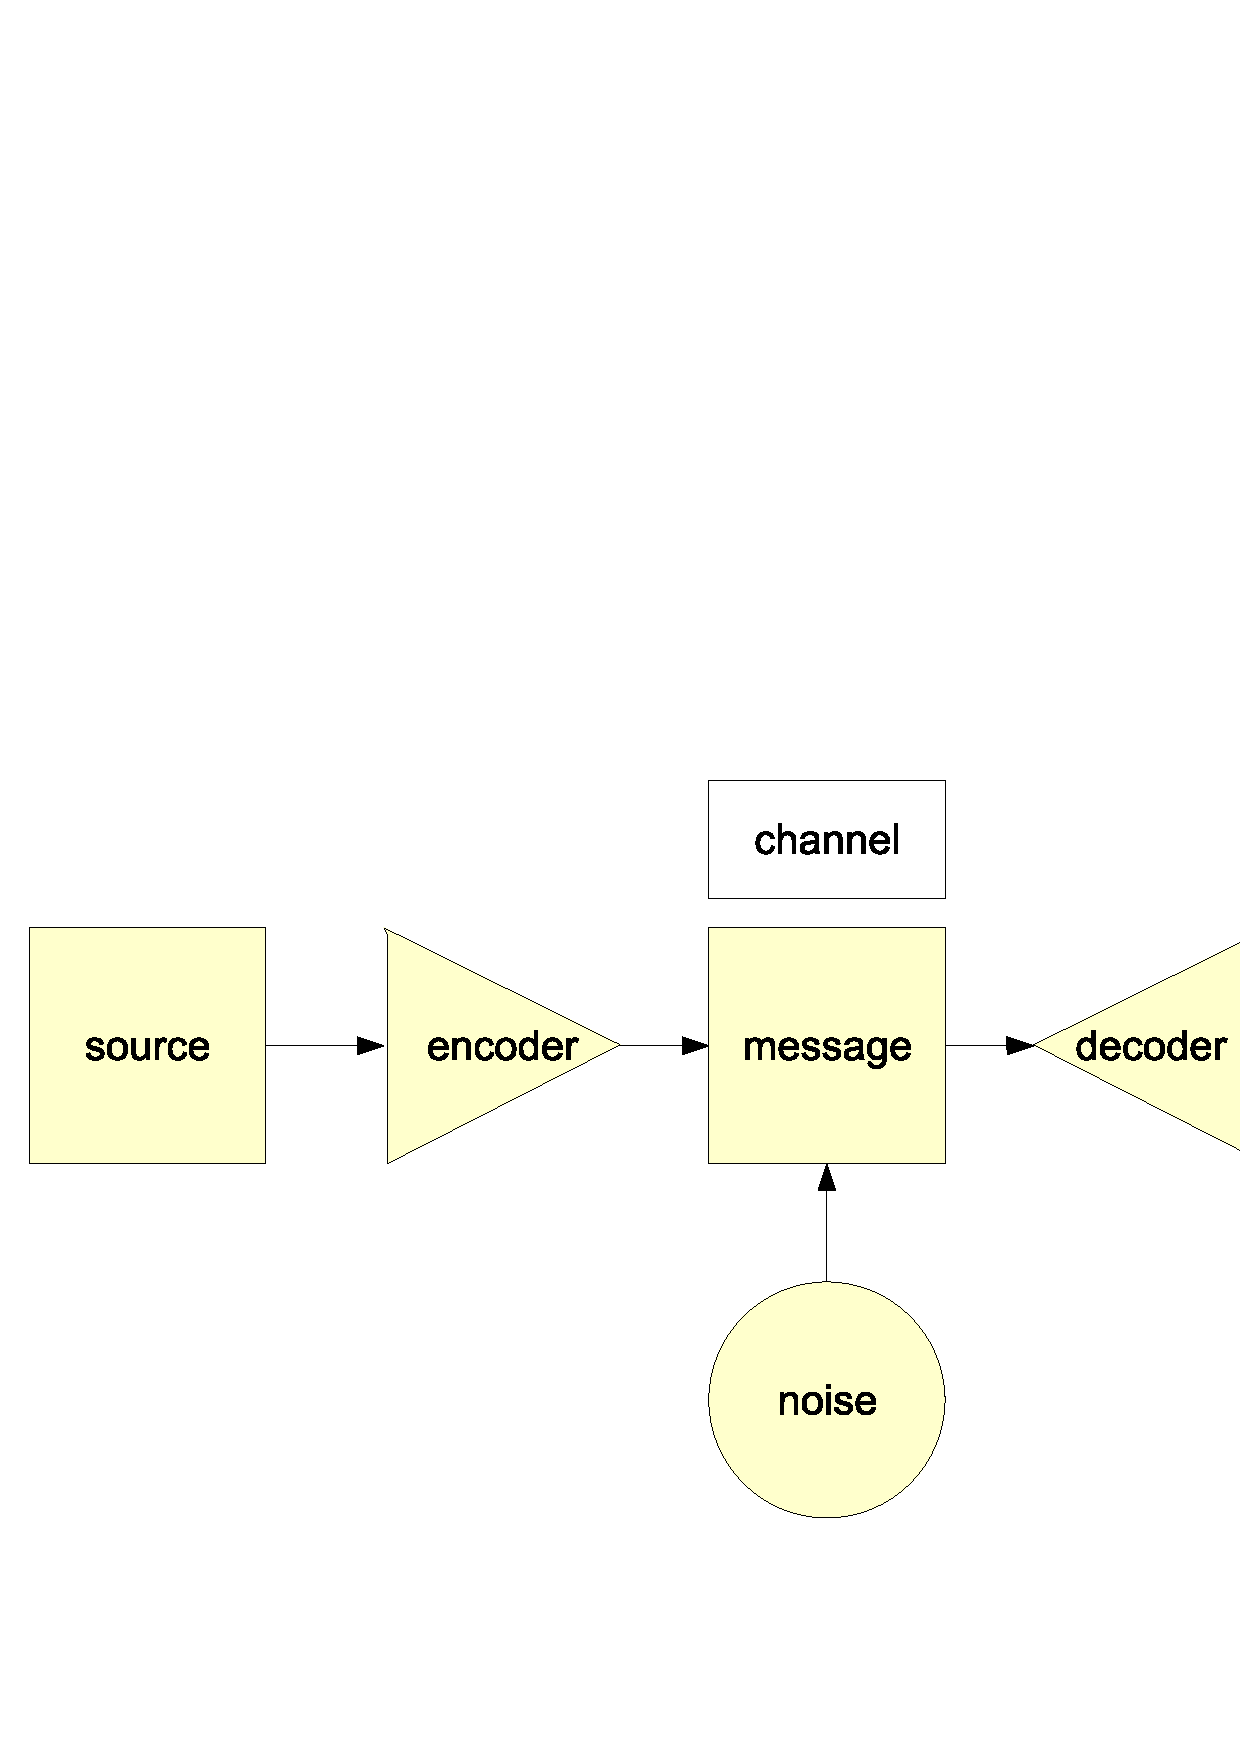
\includegraphics[scale=0.3,angle=-90]{graphic/shannon.pdf}
        \caption{Mathematical Communication Model by Shannon \& Weaver \cite{shannon}}
        \label{shannon_figure}
    \end{center}
\end{figure}

The \emph{Conversation Model} of Osgood \& Schramm (figure \ref{osgood_figure})
extends the communication model to a circular process of \emph{Question} and
\emph{Answer}, of \emph{Sending} and \emph{Receiving}. It shows more clearly,
that \emph{every} system, in order to communicate both ways, needs to own an
\emph{encoding} as well as a \emph{decoding} translator. The interpreter system
introduced in chapter \ref{cybernetics_oriented_interpreter_heading} contains
both kinds of translators.

\begin{figure}[ht]
    \begin{center}
        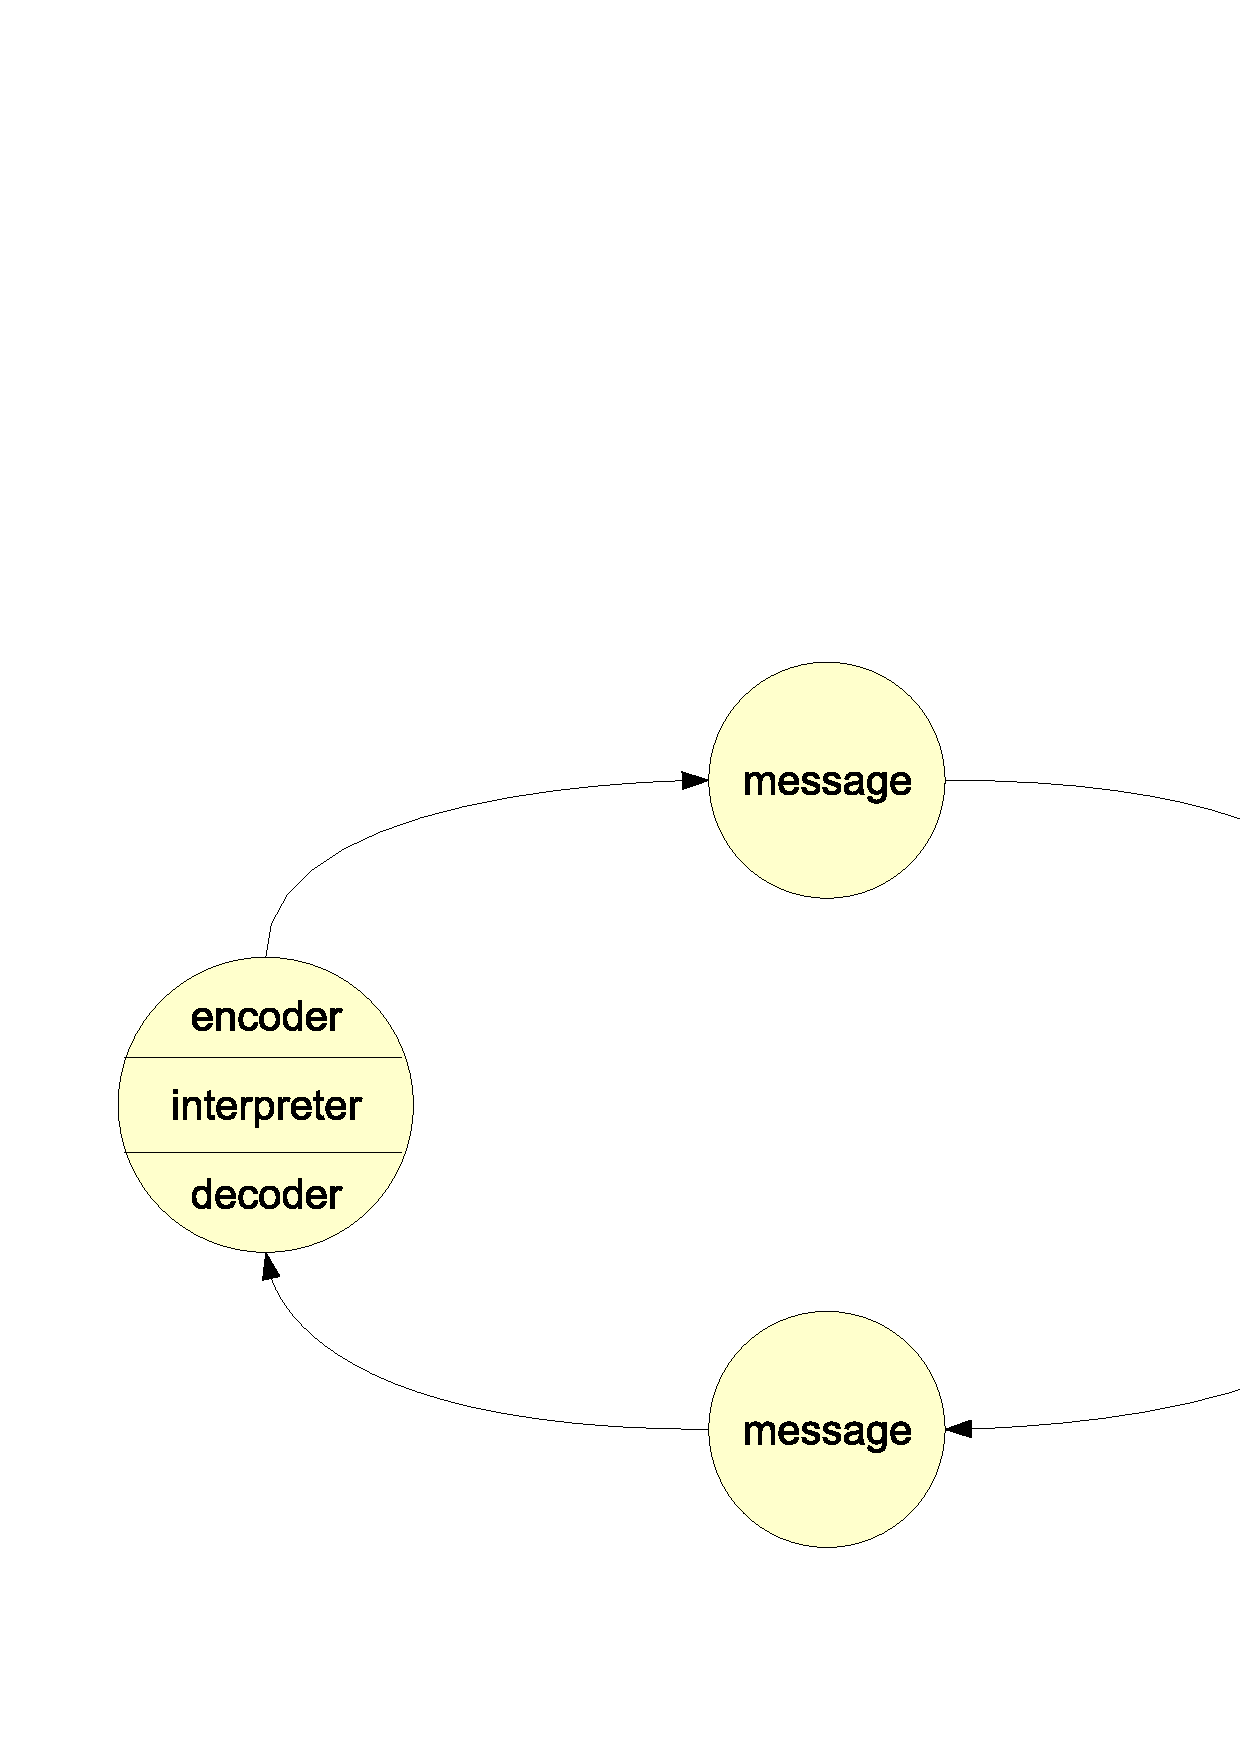
\includegraphics[scale=0.3,angle=-90]{graphic/osgood.pdf}
        \caption{Conversation Model by Osgood \& Schramm \cite{osgood}}
        \label{osgood_figure}
    \end{center}
\end{figure}

The \emph{Contents of Communication} is described by the
\emph{Lasswell Formula} (figure \ref{lasswell_figure}). After it, communication
consists of the five elements: \emph{Sender} (Who) and \emph{Receiver} (Whom),
\emph{Message} (What), \emph{Language} (Channel) and \emph{Result} (Effect).
The first four of these will be considered in the specification of the
knowledge modelling language introduced in chapter
\ref{cybernetics_oriented_language_heading}. The effects a communication has
(fifth element) are not a prerequisite for that communication to happen and
thus not interesting in the context of its technical realisation, as
investigated later in this work.

\begin{figure}[ht]
    \begin{center}
        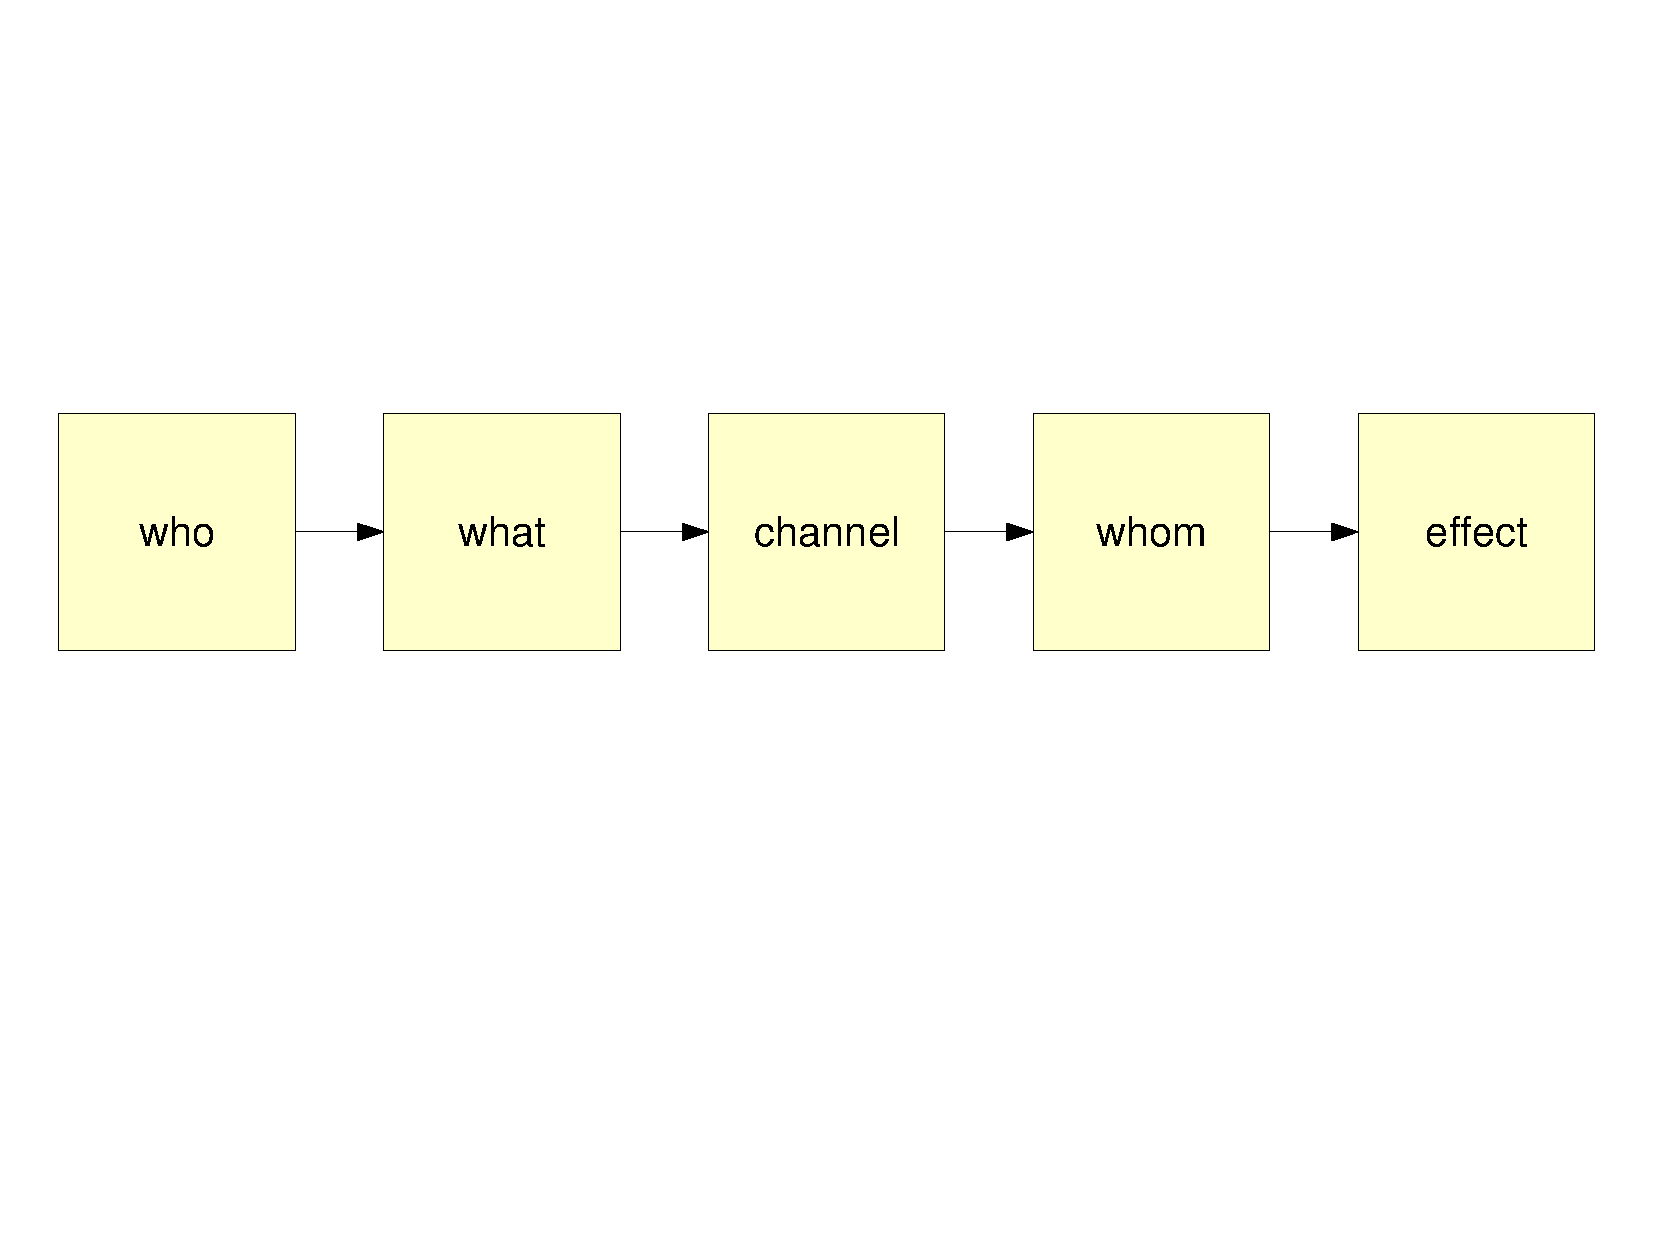
\includegraphics[scale=0.3,angle=-90]{graphic/lasswell.pdf}
        \caption{Contents of Communication (Lasswell Formula) \cite{lasswell}}
        \label{lasswell_figure}
    \end{center}
\end{figure}


\input{shell_commands}

    \newpage{\pagestyle{empty}\cleardoublepage}
    %
% $RCSfile: examples.tex,v $
%
% Copyright (c) 2002-2007. Christian Heller. All rights reserved.
%
% Permission is granted to copy, distribute and/or modify this document
% under the terms of the GNU Free Documentation License, Version 1.1 or
% any later version published by the Free Software Foundation; with no
% Invariant Sections, with no Front-Cover Texts and with no Back-Cover
% Texts. A copy of the license is included in the section entitled
% "GNU Free Documentation License".
%
% http://www.cybop.net
% - Cybernetics Oriented Programming -
%
% Version: $Revision: 1.1 $ $Date: 2007-08-01 13:59:00 $ $Author: christian $
% Authors: Christian Heller <christian.heller@tuxtax.de>
%

\chapter{Examples}
\label{examples_heading}
\index{Examples}

The following examples demonstrate how CYBOL's constructs may be used in
practice. Also, attention is payed to how control structures of classical
programming languages may be implemented in CYBOL. Furthermore, this section
discusses how inheritance, containers and software patterns were considered in
the design of CYBOL.

%
% $RCSfile: state_examples.tex,v $
%
% Copyright (C) 2002-2008. Christian Heller.
%
% Permission is granted to copy, distribute and/or modify this document
% under the terms of the GNU Free Documentation License, Version 1.1 or
% any later version published by the Free Software Foundation; with no
% Invariant Sections, with no Front-Cover Texts and with no Back-Cover
% Texts. A copy of the license is included in the section entitled
% "GNU Free Documentation License".
%
% http://www.cybop.net
% - Cybernetics Oriented Programming -
%
% http://www.resmedicinae.org
% - Information in Medicine -
%
% Version: $Revision: 1.1 $ $Date: 2008-08-19 20:41:09 $ $Author: christian $
% Authors: Christian Heller <christian.heller@tuxtax.de>
%

\subsection{State Examples}
\label{state_examples_heading}
\index{CYBOL State Example Constructs}

The creation of composed state models is quite straightforward and clear, as
the following CYBOL knowledge templates show.

%
% $RCSfile: model_part_relation.tex,v $
%
% Copyright (c) 2002-2007. Christian Heller. All rights reserved.
%
% Permission is granted to copy, distribute and/or modify this document
% under the terms of the GNU Free Documentation License, Version 1.1 or
% any later version published by the Free Software Foundation; with no
% Invariant Sections, with no Front-Cover Texts and with no Back-Cover
% Texts. A copy of the license is included in the section entitled
% "GNU Free Documentation License".
%
% http://www.cybop.net
% - Cybernetics Oriented Programming -
%
% Version: $Revision: 1.1 $ $Date: 2007-08-01 13:59:00 $ $Author: christian $
% Authors: Christian Heller <christian.heller@tuxtax.de>
%

\subsection{Model-Part Relation}
\label{model_part_relation_heading}
\index{Model-Part Relation Example}
\index{DocBook DTD}
\index{The Linux Documentation Project}
\index{TLDP}

The DocBook DTD \cite{docbook} is one of many well-known specifications for
structuring documents. The Linux Documentation Project (TLDP) \cite{linuxdoc}
makes heavy use of it. DocBook is based on numerous XML tags with defined
meaning. The following example shows how parts of a \emph{Text Document} can be
modelled differently, with at most four tags, using CYBOL:

\begin{scriptsize}
    \begin{verbatim}
<model>
    <part name="title" channel="inline" abstraction="string" model="Quo Vadis"/>
    <part name="author" channel="inline" abstraction="string" model="Henryk Sienkiewicz"/>
    <part name="date" channel="inline" abstraction="date" model="1896-01-01"/>
    <part name="contents" channel="file" abstraction="cybol" model="contents.cybol"/>
    <part name="chapter_$1" channel="file" abstraction="cybol" model="chapter_1.cybol"/>
    <part name="chapter_$2" channel="file" abstraction="cybol" model="chapter_2.cybol"/>
    <part name="chapter_$3" channel="file" abstraction="cybol" model="chapter_3.cybol"/>
    <part name="appendix" channel="file" abstraction="cybol" model="appendix.cybol"/>
</model>
    \end{verbatim}
\end{scriptsize}

%
% $RCSfile: meta_properties.tex,v $
%
% Copyright (C) 2002-2008. Christian Heller.
%
% Permission is granted to copy, distribute and/or modify this document
% under the terms of the GNU Free Documentation License, Version 1.1 or
% any later version published by the Free Software Foundation; with no
% Invariant Sections, with no Front-Cover Texts and with no Back-Cover
% Texts. A copy of the license is included in the section entitled
% "GNU Free Documentation License".
%
% http://www.cybop.net
% - Cybernetics Oriented Programming -
%
% http://www.resmedicinae.org
% - Information in Medicine -
%
% Version: $Revision: 1.1 $ $Date: 2008-08-19 20:41:07 $ $Author: christian $
% Authors: Christian Heller <christian.heller@tuxtax.de>
%

\subsubsection{Meta Properties}
\label{meta_properties_heading}
\index{CYBOL Meta Property Example}
\index{Graphical User Interface}
\index{GUI}
\index{Java Swing Framework}
\index{GUI Layouts}

When modelling \emph{Graphical User Interfaces} (GUI), a speciality to take
care about is the \emph{Position} of GUI elements within their surrounding
container. GUI components may have very different orderings and positions. The
\emph{Java Swing} framework \cite{java}, for example, offers \emph{BorderLayout},
\emph{BoxLayout}, \emph{CardLayout}, \emph{FlowLayout}, \emph{GridBagLayout} etc.

The following example of a GUI \emph{Dialogue} assumes that an interpreter
knows how to handle \emph{Compass} layouts, which are the pendant of the
above-mentioned \emph{BorderLayout}:

\begin{scriptsize}
    \begin{verbatim}
<model>
    <part name="title" channel="inline" abstraction="string" model="Prescription Dialogue"/>
    <part name="menu_bar" channel="file" abstraction="cybol" model="menu_bar.cybol">
        <property name="position" channel="inline" abstraction="string" model="north"/>
    </part>
    <part name="tool_bar" channel="file" abstraction="cybol" model="tool_bar.cybol">
        <property name="position" channel="inline" abstraction="string" model="west"/>
    </part>
    <part name="contents_panel" channel="file" abstraction="cybol" model="contents_panel.cybol">
        <property name="position" channel="inline" abstraction="string" model="centre"/>
    </part>
    <part name="status_bar" channel="file" abstraction="cybol" model="status_bar.cybol">
        <property name="position" channel="inline" abstraction="string" model="south"/>
    </part>
</model>
    \end{verbatim}
\end{scriptsize}

Further meta information such as the \emph{Colour} or \emph{Size} of a GUI
component may be given. The following example shows how a GUI \emph{Button} may
be modelled as part of some GUI panel. Again, properties like \emph{size} are
not modelled as part, because the button does not \emph{consist} of them, in a
structural way of thinking:

\begin{scriptsize}
    \begin{verbatim}
<model>
    <part name="exit_button" channel="file" abstraction="cybol" model="exit_button.cybol">
        <property name="position" channel="inline" abstraction="integer" model="0"/>
        <property name="size" channel="inline" abstraction="vector" model="80,20,1"/>
        <property name="colour" channel="inline" abstraction="rgb" model="127,127,127"/>
        <property name="action" channel="inline" abstraction="string" model="exit.cybol"/>
    </part>
</model>
    \end{verbatim}
\end{scriptsize}

%
% $RCSfile: external_resources.tex,v $
%
% Copyright (C) 2002-2008. Christian Heller.
%
% Permission is granted to copy, distribute and/or modify this document
% under the terms of the GNU Free Documentation License, Version 1.1 or
% any later version published by the Free Software Foundation; with no
% Invariant Sections, with no Front-Cover Texts and with no Back-Cover
% Texts. A copy of the license is included in the section entitled
% "GNU Free Documentation License".
%
% http://www.cybop.net
% - Cybernetics Oriented Programming -
%
% http://www.resmedicinae.org
% - Information in Medicine -
%
% Version: $Revision: 1.1 $ $Date: 2008-08-19 20:41:06 $ $Author: christian $
% Authors: Christian Heller <christian.heller@tuxtax.de>
%

\subsubsection{External Resources}
\label{external_resources_heading}
\index{CYBOL External Resources Example}
\index{Encapsulated PostScript}
\index{EPS}
\index{Hyper Text Transfer Protocol}
\index{HTTP}

A \emph{Text Document} like the one shown in the example above often contains
graphical illustrations called \emph{Figures}, which it may include from
external files. One common graphics format is \emph{Encapsulated PostScript}
(EPS), for example. \emph{Graphical User Interfaces} (GUI) as modelled before
do contain \emph{Icons}; a GUI button may contain a \emph{Glyph} and so forth.

CYBOL therefore offers ways for linking external resources, given in various
formats, as shown in the following hypothetical knowledge template. The last of
the template's parts retrieves its data not from a file in the local file
system, but across a \emph{Hyper Text Transfer Protocol} (HTTP) link instead:

\begin{scriptsize}
    \begin{verbatim}
<model>
    <part name="pdf_document" channel="file" abstraction="pdf" model="example.pdf"/>
    <part name="ogg_audio" channel="file" abstraction="ogg" model="example.ogg"/>
    <part name="mpeg_video" channel="file" abstraction="mpeg" model="example.mpeg"/>
    <part name="eps_image" channel="file" abstraction="eps" model="example.eps"/>
    <part name="jpeg_image" channel="http" abstraction="jpeg" model="host.domain.tld/example.jpeg"/>
</model>
    \end{verbatim}
\end{scriptsize}

%
% $RCSfile: serialised_model.tex,v $
%
% Copyright (c) 2002-2007. Christian Heller. All rights reserved.
%
% Permission is granted to copy, distribute and/or modify this document
% under the terms of the GNU Free Documentation License, Version 1.1 or
% any later version published by the Free Software Foundation; with no
% Invariant Sections, with no Front-Cover Texts and with no Back-Cover
% Texts. A copy of the license is included in the section entitled
% "GNU Free Documentation License".
%
% http://www.cybop.net
% - Cybernetics Oriented Programming -
%
% Version: $Revision: 1.1 $ $Date: 2007-08-01 13:59:00 $ $Author: christian $
% Authors: Christian Heller <christian.heller@tuxtax.de>
%

\subsection{Serialised Model}
\label{serialised_model_heading}
\index{Serialised Model Example}

A possible (but not necessarily recommended) alternative to the linking of
external resources is to store such information (as binary code) \emph{inline}
in the CYBOL knowledge template. One case in which it is necessary to store all
information inline in the model is \emph{Serialisation}.

A CYBOL address management application that does not rely on the existence of a
\emph{Database Management System} (DBMS) probably has to store addresses in
form of serialised files, such as the one shown following. It contains two
parts representing dynamically extensible lists, one for \emph{phone\_numbers}
and another one for \emph{addresses}:

\begin{scriptsize}
    \begin{verbatim}
<model>
    <part name="honorific_prefix" channel="inline" abstraction="string" model="Dr."/>
    <part name="given_name" channel="inline" abstraction="string" model="Tux"/>
    <part name="family_name" channel="inline" abstraction="string" model="Penguin"/>
    <part name="phone_numbers" channel="inline" abstraction="cybol" model="(
        <part name="home" channel="inline" abstraction="string" model="123"/>
        <part name="work" channel="inline" abstraction="string" model="456"/>
        <part name="mobile" channel="inline" abstraction="string" model="789"/>
    )"/>
    <part name="addresses" channel="inline" abstraction="cybol" model="(
        ...
    )"/>
</model>
    \end{verbatim}
\end{scriptsize}

The serialisation of CYBOL models causes one problem: Due to the double
hierarchy to which belong \emph{Whole-Part} relations (stored in XML attributes)
and \emph{Meta Information} (stored in XML tags), it is not possible to store
CYBOL models in an XML-conform manner. Instead of referencing external files
containing the corresponding CYBOL \emph{Part} models, a serialised
\emph{Whole} model has to contain these inline.

While XML tags were invented as pairs consisting of a \emph{begin} and an
\emph{end} tag, XML attribute values are enclosed by simple quotation marks.
Hence, the beginning markup of an attribute value does not look any different
than its ending markup. This is a true problem, because serialised whole-part
hierarchies of CYBOL models, with attribute values containing complete sub
models with their own attributes, would get completely mixed up in pure XML
notation.

It was therefore inevitable to break XML-conformity and introduce two
additional markup tokens \emph{"(} and \emph{)"}, indicating the beginning and
end of an XML attribute value. The tokens are extensions of the quotation marks
of standard XML attributes, with one left/ right parenthesis, respectively.
That way, the degree to which attributes are nested becomes countable and it is
always clear to which tag an attribute belongs.

%
% $RCSfile: meta_constraints.tex,v $
%
% Copyright (C) 2002-2008. Christian Heller.
%
% Permission is granted to copy, distribute and/or modify this document
% under the terms of the GNU Free Documentation License, Version 1.1 or
% any later version published by the Free Software Foundation; with no
% Invariant Sections, with no Front-Cover Texts and with no Back-Cover
% Texts. A copy of the license is included in the section entitled
% "GNU Free Documentation License".
%
% http://www.cybop.net
% - Cybernetics Oriented Programming -
%
% http://www.resmedicinae.org
% - Information in Medicine -
%
% Version: $Revision: 1.1 $ $Date: 2008-08-19 20:41:07 $ $Author: christian $
% Authors: Christian Heller <christian.heller@tuxtax.de>
%

\subsubsection{Meta Constraints}
\label{meta_constraints_heading}
\index{CYBOL Meta Constraints Example}
\index{Debian GNU/Linux Package Definition}

The example of this section shows a possible \emph{Debian GNU/Linux}
\cite{debian} \emph{Package} definition, written in CYBOL:

\begin{scriptsize}
    \begin{verbatim}
<model>
    <part name="name" channel="inline" abstraction="string" model="resmedicinae"/>
    <part name="version" channel="inline" abstraction="string" model="0.1.0.0"/>
    <part name="section" channel="inline" abstraction="string" model="science"/>
    <part name="priority" channel="inline" abstraction="string" model="optional"/>
    <part name="architecture" channel="inline" abstraction="string" model="all"/>
    <part name="packages" channel="file" abstraction="cybol" model="resmedicinae-packages"/>
    <part name="files" channel="file" abstraction="cybol" model="resmedicinae-files"/>
    <part name="maintainer" channel="inline" abstraction="string" model="Happy Coder"/>
    <part name="description" channel="inline" abstraction="string" model="Medical System"/>
</model>
    \end{verbatim}
\end{scriptsize}

The part called \emph{packages} in the example above references an external
CYBOL knowledge template, which is displayed below. It represents a list of
packages having different versions and varying strengths of dependency. The
\emph{strength} property of the last of these packages has the model value
\emph{suggests} and, it contains meta information about that property, namely
a \emph{constraint}. Constraints can be, for example: minima, maxima or a
choice of possible values, as in this case.

\begin{scriptsize}
    \begin{verbatim}
<model>
    <part name="cyboi" channel="inline" abstraction="string" model="cyboi">
        <property name="strength" channel="inline" abstraction="string" model="depends"/>
        <property name="version" channel="inline" abstraction="string" model=">= 1.0.0.0"/>
        <property name="conflicts" channel="inline" abstraction="string" model="< 1.0.0.0"/>
    </part>
    <part name="cybol-healthcare" channel="inline" abstraction="string" model="cybol-healthcare">
        <property name="strength" channel="inline" abstraction="string" model="depends"/>
        <property name="version" channel="inline" abstraction="string" model=">= 0.1.0.0"/>
    </part>
    <part name="resadmin" channel="inline" abstraction="string" model="resadmin">
        <property name="strength" channel="inline" abstraction="string" model="recommends"/>
        <property name="version" channel="inline" abstraction="string" model=">= 0.8.0.0"/>
    </part>
    <part name="resmedicinae-doc" channel="inline" abstraction="string" model="resmedicinae-doc">
        <property name="strength" channel="inline" abstraction="string" model="suggests">
            <constraint name="choice" channel="inline" abstraction="set" model="suggests,recommends"/>
        </property>
        <property name="version" channel="inline" abstraction="string" model=">= 0.1.0.0"/>
    </part>
</model>
    \end{verbatim}
\end{scriptsize}


%
% $RCSfile: logic_examples.tex,v $
%
% Copyright (C) 2002-2008. Christian Heller.
%
% Permission is granted to copy, distribute and/or modify this document
% under the terms of the GNU Free Documentation License, Version 1.1 or
% any later version published by the Free Software Foundation; with no
% Invariant Sections, with no Front-Cover Texts and with no Back-Cover
% Texts. A copy of the license is included in the section entitled
% "GNU Free Documentation License".
%
% http://www.cybop.net
% - Cybernetics Oriented Programming -
%
% http://www.resmedicinae.org
% - Information in Medicine -
%
% Version: $Revision: 1.1 $ $Date: 2008-08-19 20:41:07 $ $Author: christian $
% Authors: Christian Heller <christian.heller@tuxtax.de>
%

\subsection{Logic Examples}
\label{logic_examples_heading}
\index{CYBOL Logic Example Constructs}

The CYBOL implementation of logic models (chapter \ref{state_and_logic_heading})
needs more detailed explanation, in particular the use of special control
structures as known from \emph{Structured and Procedural Programming} (SPP)
(section \ref{structured_and_procedural_programming_heading}).

%
% $RCSfile: operation_call.tex,v $
%
% Copyright (C) 2002-2008. Christian Heller.
%
% Permission is granted to copy, distribute and/or modify this document
% under the terms of the GNU Free Documentation License, Version 1.1 or
% any later version published by the Free Software Foundation; with no
% Invariant Sections, with no Front-Cover Texts and with no Back-Cover
% Texts. A copy of the license is included in the section entitled
% "GNU Free Documentation License".
%
% http://www.cybop.net
% - Cybernetics Oriented Programming -
%
% http://www.resmedicinae.org
% - Information in Medicine -
%
% Version: $Revision: 1.1 $ $Date: 2008-08-19 20:41:08 $ $Author: christian $
% Authors: Christian Heller <christian.heller@tuxtax.de>
%

\subsubsection{Operation Call}
\label{operation_call_heading}
\index{CYBOL Operation Call Example}

As stated previously, logic models may access and manipulate state models. The
simplest form of a logic model is an operation with associated input/ output
(i/o) state models. The following CYBOL knowledge template calls an \emph{add}
operation, handing over i/o parameters as \emph{properties} of the
corresponding \emph{part}:

\begin{scriptsize}
    \begin{verbatim}
<model>
    <part name="addition" channel="inline" abstraction="operation" model="add">
        <property name="summand_1" channel="inline" abstraction="integer" model="1"/>
        <property name="summand_2" channel="inline" abstraction="knowledge" model="domain.summand"/>
        <property name="sum" channel="inline" abstraction="knowledge" model="domain.result"/>
    </part>
</model>
    \end{verbatim}
\end{scriptsize}

The example nicely shows how state models can be given in various formats. The
\emph{summand\_1} is given as constant value, defined directly in the knowledge
template. Its type of abstraction is \emph{integer}. The \emph{summand\_2-} and
\emph{sum} parameters, on the other hand, are given as dot-separated references
to the runtime tree of knowledge models. Their type of abstraction is therefore
\emph{knowledge}.

%
% $RCSfile: algorithm_division.tex,v $
%
% Copyright (c) 2002-2007. Christian Heller. All rights reserved.
%
% Permission is granted to copy, distribute and/or modify this document
% under the terms of the GNU Free Documentation License, Version 1.1 or
% any later version published by the Free Software Foundation; with no
% Invariant Sections, with no Front-Cover Texts and with no Back-Cover
% Texts. A copy of the license is included in the section entitled
% "GNU Free Documentation License".
%
% http://www.cybop.net
% - Cybernetics Oriented Programming -
%
% Version: $Revision: 1.1 $ $Date: 2007-08-01 13:59:00 $ $Author: christian $
% Authors: Christian Heller <christian.heller@tuxtax.de>
%

\subsection{Algorithm Division}
\label{algorithm_division_heading}
\index{Algorithm Division Example}

Compound logic models like \emph{Algorithms}, which SPP languages implement
using nested \emph{Blocks}, can be expressed in CYBOL as well. It does not
provide blocks in the classical sense, but its hierarchical structure allows to
subdivide compound knowledge templates, and to cascade compound logic as well
as primitive operations. The following example calls an addition operation,
before a compound algorithm, situated in an external CYBOL file, gets executed:

\begin{scriptsize}
    \begin{verbatim}
<model>
    <part name="addition" channel="inline" abstraction="operation" model="add">
        <property name="summand_1" channel="inline" abstraction="knowledge" model="domain.number_1"/>
        <property name="summand_2" channel="inline" abstraction="knowledge" model="domain.number_2"/>
        <property name="sum" channel="inline" abstraction="knowledge" model="domain.number_3"/>
    </part>
    <part name="algorithm" channel="file" abstraction="cybol" model="logic/algorithm.cybol"/>
</model>
    \end{verbatim}
\end{scriptsize}

%
% $RCSfile: simple_assignment.tex,v $
%
% Copyright (c) 2002-2007. Christian Heller. All rights reserved.
%
% Permission is granted to copy, distribute and/or modify this document
% under the terms of the GNU Free Documentation License, Version 1.1 or
% any later version published by the Free Software Foundation; with no
% Invariant Sections, with no Front-Cover Texts and with no Back-Cover
% Texts. A copy of the license is included in the section entitled
% "GNU Free Documentation License".
%
% http://www.cybop.net
% - Cybernetics Oriented Programming -
%
% Version: $Revision: 1.1 $ $Date: 2007-08-01 13:59:00 $ $Author: christian $
% Authors: Christian Heller <christian.heller@tuxtax.de>
%

\subsection{Simple Assignment}
\label{simple_assignment_heading}
\index{Simple Assignment Example}

CYBOL does not know \emph{Variables} as used in classical languages. All states
a system may take on are represented by just one \emph{Knowledge Tree}, which
applications may access in a defined manner (dot-separated knowledge paths).
Consequently, \emph{Assignments} are done differently in CYBOL than in
classical programming languages. All kinds of state changes go back to a
manipulation of the one knowledge tree:

\begin{scriptsize}
    \begin{verbatim}
<model>
    <part name="copy_value" channel="inline" abstraction="operation" model="copy">
        <property name="source" channel="inline" abstraction="knowledge" model="domain.name"/>
        <property name="destination" channel="inline" abstraction="knowledge" model="gui.name"/>
    </part>
    <part name="move_branch" channel="inline" abstraction="operation" model="move">
        <property name="source" channel="inline" abstraction="knowledge" model="address_1.phone"/>
        <property name="destination" channel="inline" abstraction="knowledge" model="address_2"/>
    </part>
</model>
    \end{verbatim}
\end{scriptsize}

The first operation in the example above copies a value between two branches of
the tree. Only primitive values can be copied. The second operation removes a
whole tree branch (referenced by the \emph{source} property) from one parent
node, and adds it to another (referenced by the \emph{destination} property).

%
% $RCSfile: loop_as_operation.tex,v $
%
% Copyright (c) 2002-2007. Christian Heller. All rights reserved.
%
% Permission is granted to copy, distribute and/or modify this document
% under the terms of the GNU Free Documentation License, Version 1.1 or
% any later version published by the Free Software Foundation; with no
% Invariant Sections, with no Front-Cover Texts and with no Back-Cover
% Texts. A copy of the license is included in the section entitled
% "GNU Free Documentation License".
%
% http://www.cybop.net
% - Cybernetics Oriented Programming -
%
% Version: $Revision: 1.1 $ $Date: 2007-08-01 13:59:00 $ $Author: christian $
% Authors: Christian Heller <christian.heller@tuxtax.de>
%

\subsection{Loop as Operation}
\label{loop_as_operation_heading}
\index{Loop as Operation Example}

\emph{Looping} is a major technique for the effective processing of whole
stacks of data. As many other control structures, it is simplified to a logic
operation, in CYBOL.

\begin{figure}[ht]
    \begin{center}
        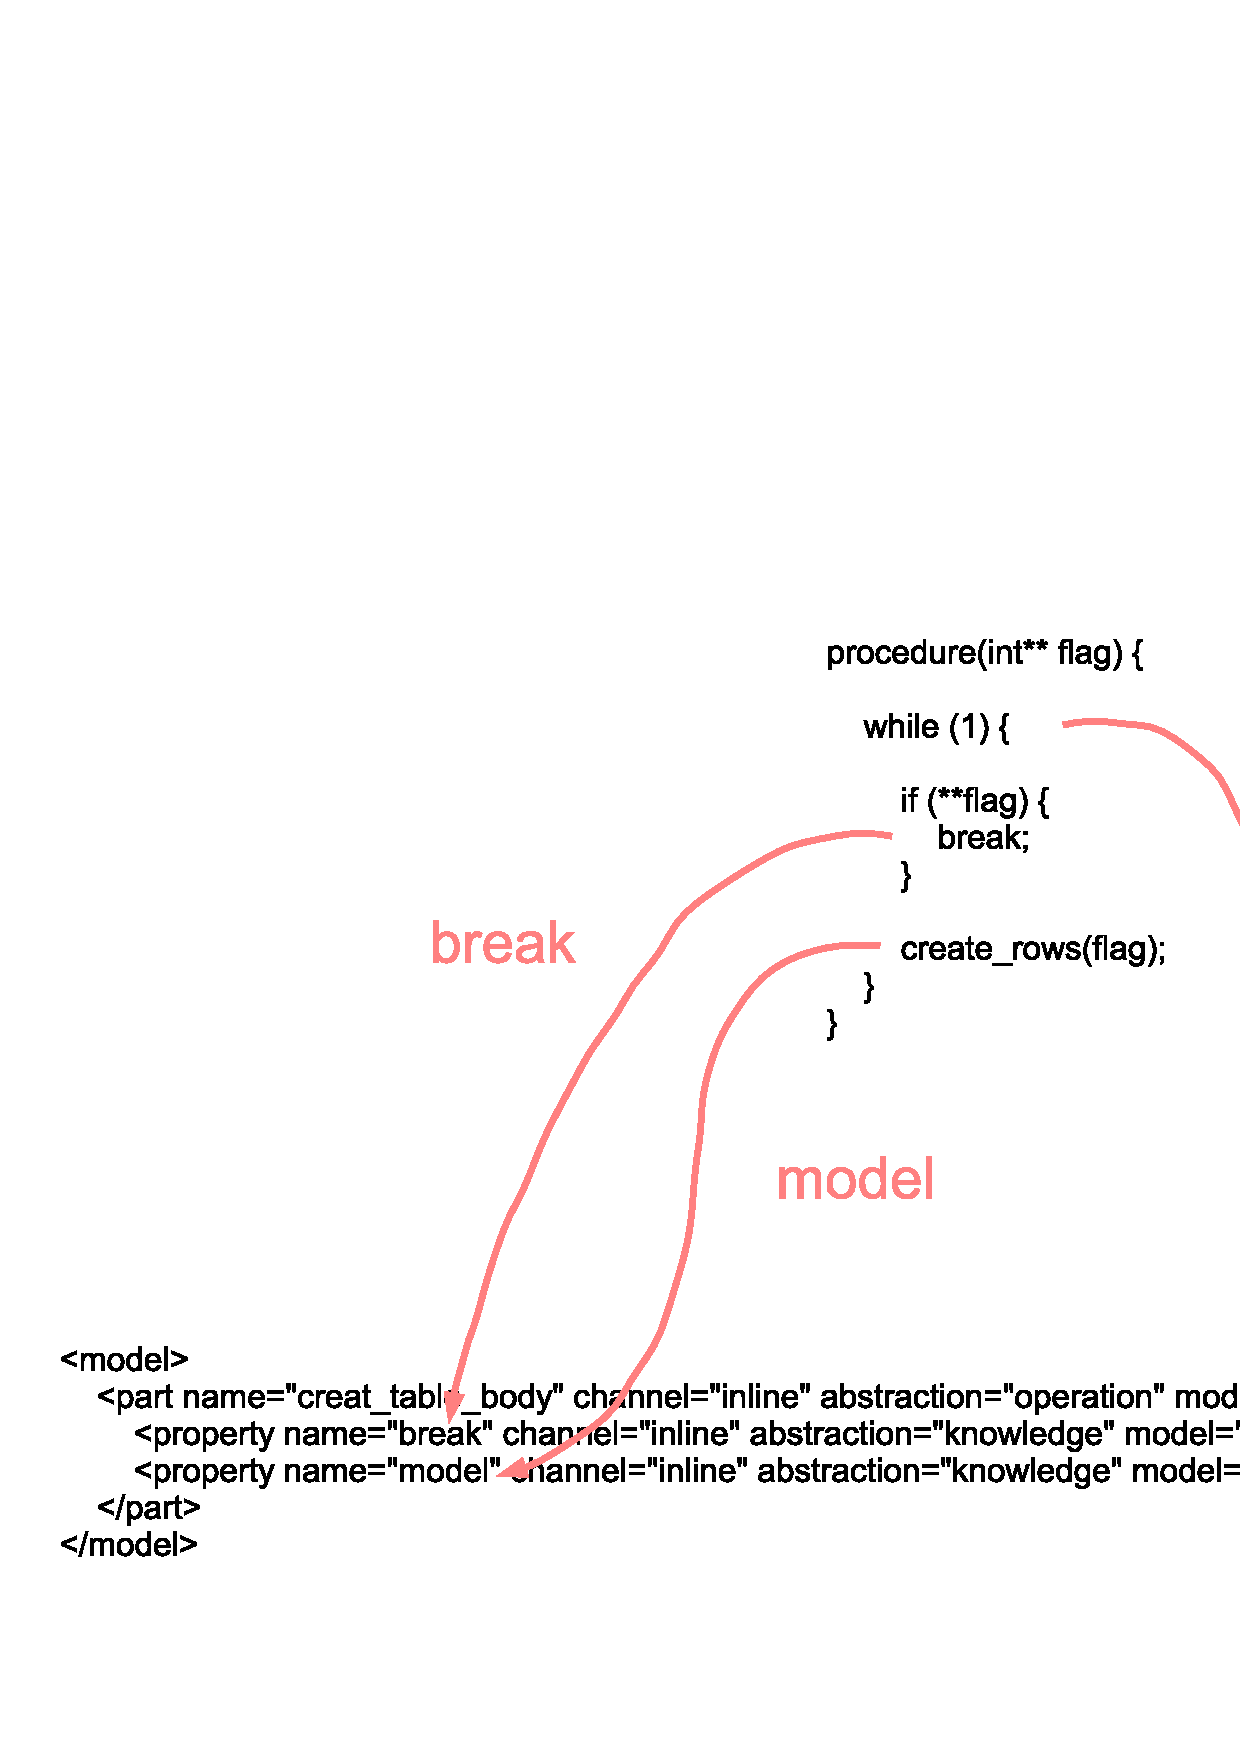
\includegraphics[scale=0.3,angle=-90]{graphics/cybolloop.pdf}
        \caption{Loop Control Structure and Elements in C and CYBOL}
        \label{cybolloop_figure}
    \end{center}
\end{figure}

The \emph{loop} operation needs two parameters to be functional: a \emph{break}
flag as means of interruption and a logic \emph{model} to be executed in each
loop cycle (figure \ref{cybolloop_figure}). An \emph{index} counting loop
cycles is not given, as it is in the responsibility of the logic \emph{model}
to manage that index, just like the setting of the \emph{break} flag,
internally. The following example dynamically creates a table consisting of a
number of rows:

\begin{scriptsize}
    \begin{verbatim}
<model>
    <part name="creat_table_body" channel="inline" abstraction="operation" model="loop">
        <property name="break" channel="inline" abstraction="knowledge" model=".domain.flag"/>
        <property name="model" channel="inline" abstraction="knowledge" model=".logic.create_rows"/>
    </part>
</model>
    \end{verbatim}
\end{scriptsize}

%
% $RCSfile: conditional_execution.tex,v $
%
% Copyright (c) 2002-2007. Christian Heller. All rights reserved.
%
% Permission is granted to copy, distribute and/or modify this document
% under the terms of the GNU Free Documentation License, Version 1.1 or
% any later version published by the Free Software Foundation; with no
% Invariant Sections, with no Front-Cover Texts and with no Back-Cover
% Texts. A copy of the license is included in the section entitled
% "GNU Free Documentation License".
%
% http://www.cybop.net
% - Cybernetics Oriented Programming -
%
% Version: $Revision: 1.1 $ $Date: 2007-08-01 13:59:00 $ $Author: christian $
% Authors: Christian Heller <christian.heller@tuxtax.de>
%

\subsection{Conditional Execution}
\label{conditional_execution_heading}
\index{Conditional Execution Example}

An obviously presupposed part in the previous example is a logic setting the
break \emph{condition} (flag). If the break flag was not set, the loop would
run endlessly. The following knowledge template therefore shows a
\emph{comparison} operation, as it could stand at the end of the loop's logic
model, referenced by the \emph{model} property in the previous example. After
having compared the current loop index with a maximum loop count number, the
break flag may or may not be set. When entering its next cycle, the loop
operation checks whether the flag is set. If so, the loop is stopped:

\begin{scriptsize}
    \begin{verbatim}
<model>
    <part name="comparison" channel="inline" abstraction="operation" model="compare">
        <property name="operator" channel="inline" abstraction="character" model="greater_or_equal"/>
        <property name="left_side" channel="inline" abstraction="knowledge" model=".domain.index"/>
        <property name="right_side" channel="inline" abstraction="knowledge" model=".domain.count"/>
        <property name="result" channel="inline" abstraction="knowledge" model=".domain.flag"/>
    </part>
</model>
    \end{verbatim}
\end{scriptsize}

\begin{figure}[ht]
    \begin{center}
        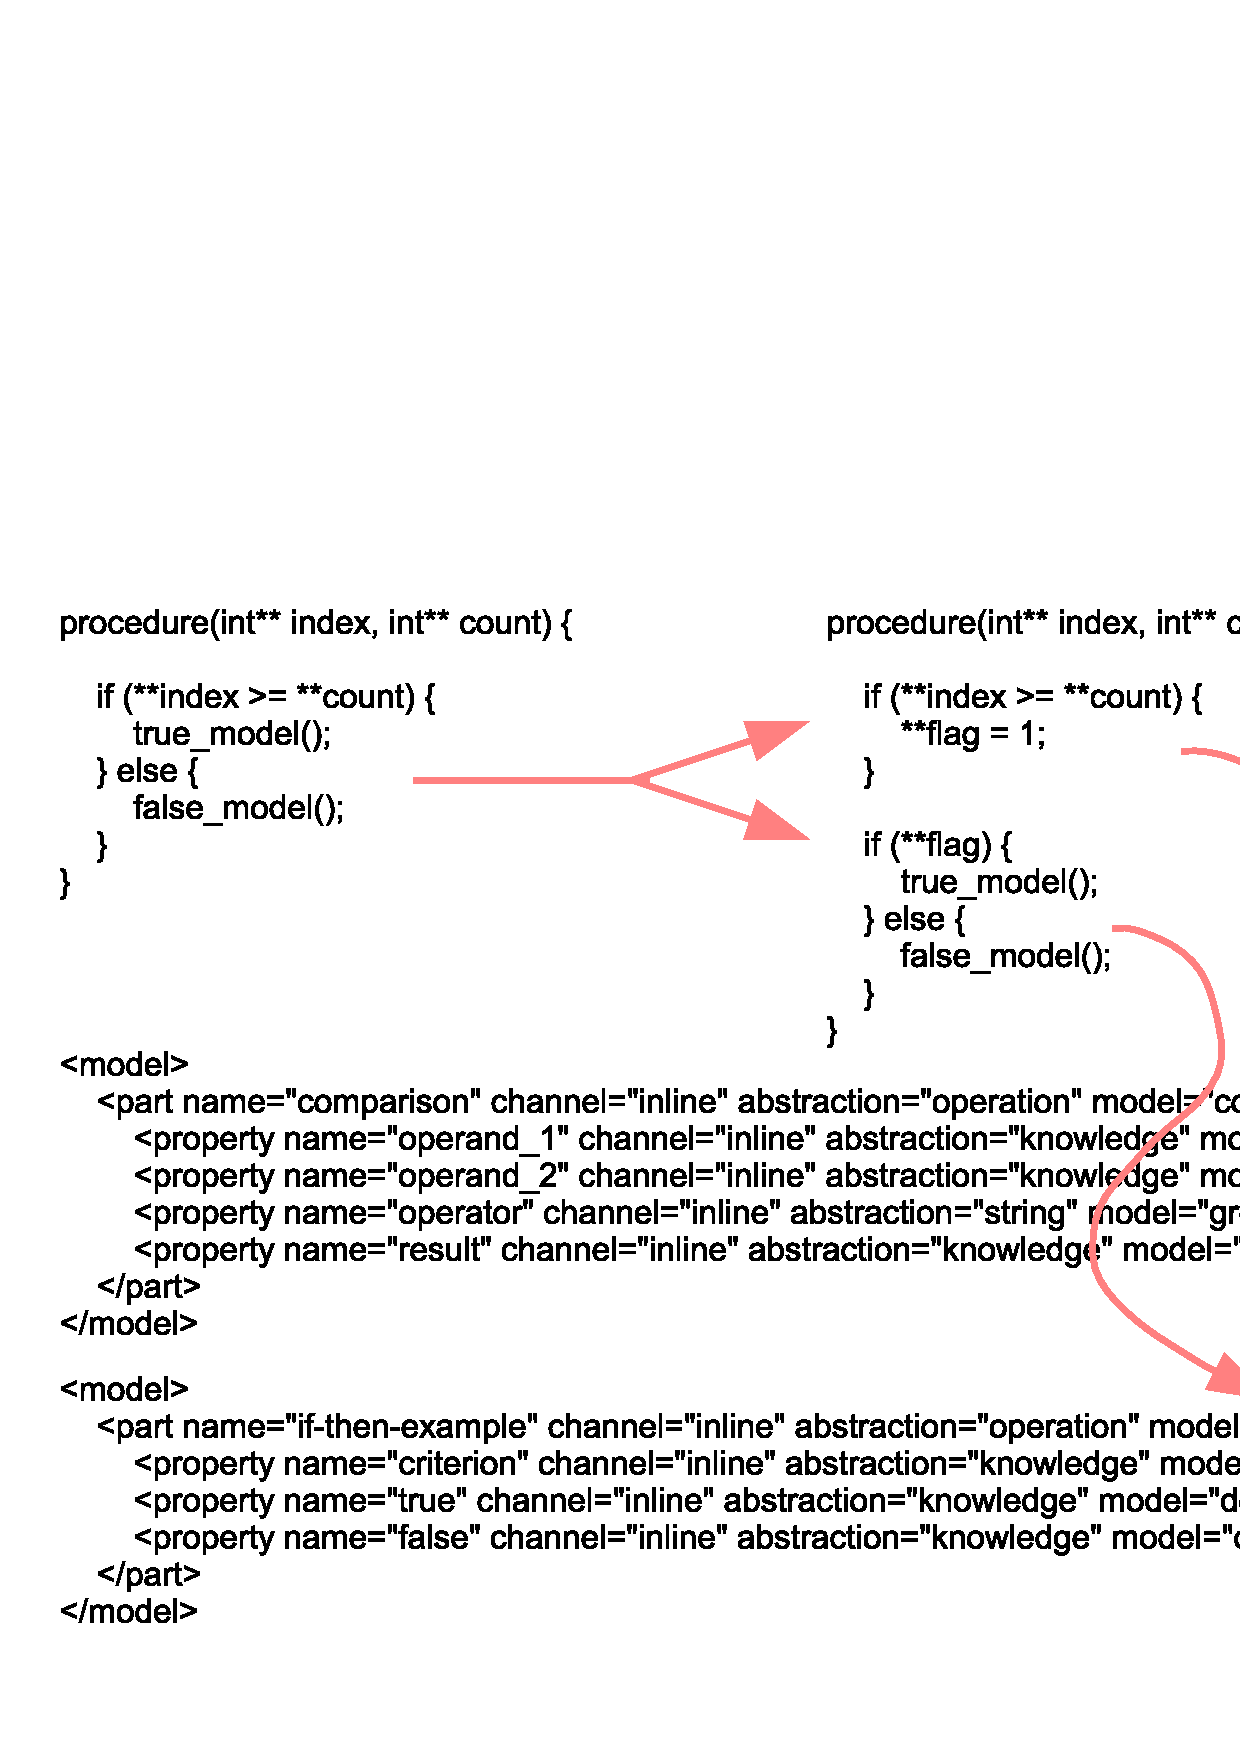
\includegraphics[scale=0.3,angle=-90]{graphics/cybolcondition.pdf}
        \caption{Condition Control Structure and Elements in C and CYBOL}
        \label{cybolcondition_figure}
    \end{center}
\end{figure}

Flags as one of the earliest techniques used in computing (in software as well
as in hardware) are the perfect means for controlling the execution of
primitive logic models, namely operations. They represent a condition set as
result of another logic model -- the latter often being some kind of comparison
operation. In order to execute code upon activation of a flag, a conventional
comparison control structure needs to be split up into two independent blocks
(figure \ref{cybolcondition_figure}), with the flag being the linking element.
The flag which was set by a comparison operation is used for branching the
control flow.

The second example shows how a classical \emph{if-then} statement would be
written in CYBOL. The corresponding operation is called \emph{branch} and it
expects three properties: a \emph{criterion} flag and two models, of which one
is executed in case the flag is \emph{true} and the other is executed otherwise.

\begin{scriptsize}
    \begin{verbatim}
<model>
    <part name="if-then-example" channel="inline" abstraction="operation" model="branch">
        <property name="criterion" channel="inline" abstraction="knowledge" model=".domain.flag"/>
        <property name="true" channel="inline" abstraction="knowledge" model=".domain.true_model"/>
        <property name="false" channel="inline" abstraction="knowledge" model=".domain.false_model"/>
    </part>
</model>
    \end{verbatim}
\end{scriptsize}


%
% $RCSfile: special_examples.tex,v $
%
% Copyright (C) 2002-2008. Christian Heller.
%
% Permission is granted to copy, distribute and/or modify this document
% under the terms of the GNU Free Documentation License, Version 1.1 or
% any later version published by the Free Software Foundation; with no
% Invariant Sections, with no Front-Cover Texts and with no Back-Cover
% Texts. A copy of the license is included in the section entitled
% "GNU Free Documentation License".
%
% http://www.cybop.net
% - Cybernetics Oriented Programming -
%
% http://www.resmedicinae.org
% - Information in Medicine -
%
% Version: $Revision: 1.1 $ $Date: 2008-08-19 20:41:09 $ $Author: christian $
% Authors: Christian Heller <christian.heller@tuxtax.de>
%

\subsection{Special Examples}
\label{special_examples_heading}
\index{CYBOL Special Example Constructs}

\emph{XML} is used for representing data of very different domains, and a whole
plethora of XML dialects exists. Two of them are mentioned following. The main
purpose of the next examples, however, is to show how CYBOL can replace these.

%
% $RCSfile: synchronous_execution.tex,v $
%
% Copyright (c) 2002-2007. Christian Heller. All rights reserved.
%
% Permission is granted to copy, distribute and/or modify this document
% under the terms of the GNU Free Documentation License, Version 1.1 or
% any later version published by the Free Software Foundation; with no
% Invariant Sections, with no Front-Cover Texts and with no Back-Cover
% Texts. A copy of the license is included in the section entitled
% "GNU Free Documentation License".
%
% http://www.cybop.net
% - Cybernetics Oriented Programming -
%
% Version: $Revision: 1.1 $ $Date: 2007-08-01 13:59:00 $ $Author: christian $
% Authors: Christian Heller <christian.heller@tuxtax.de>
%

\subsection{Synchronous Execution}
\label{synchronous_execution_heading}
\index{Synchronous Execution Example}
\index{MusicXML}

\emph{MusicXML} \cite{musicxml} is a markup language \textit{designed to
represent musical scores, specifically common western musical notation from the
17th century onwards.} In principle, CYBOL could be used for this purpose as
well. Of course, there are many details (additional properties) which would
still have to be worked out in order to be able to correctly represent complete
musical scores. As most models, the \emph{Musical Work} displayed in figure
\ref{music_figure} can be considered a hierarchy consisting of \emph{Parts}
(played/ sung by instruments/ voices). Parts in turn consist of
\emph{Measures}, which consist of \emph{Notes}, which finally have a
\emph{Pitch} and sometimes \emph{Lyric}.

\begin{figure}[ht]
    \begin{center}
        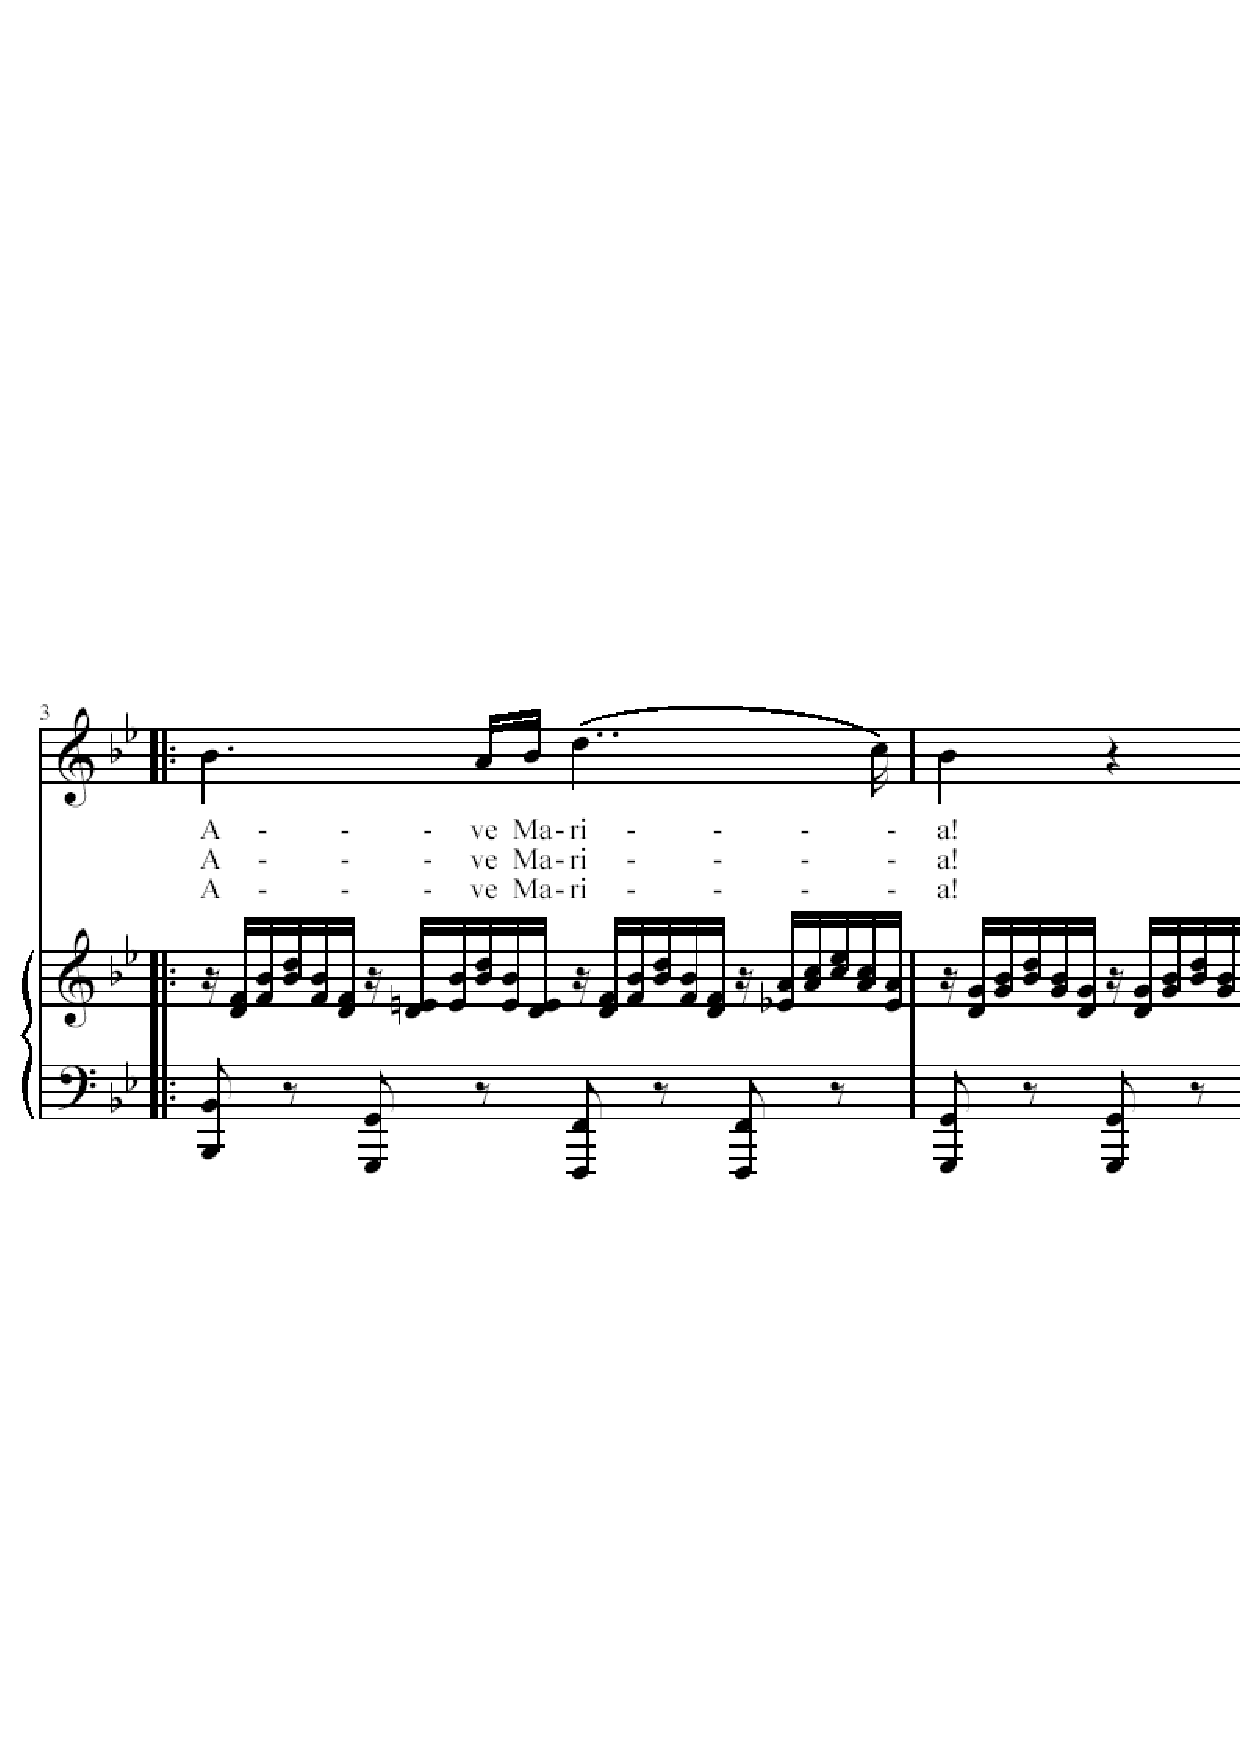
\includegraphics[scale=0.3,angle=-90]{graphics/music.pdf}
%        \caption{Musical Score of Franz Schubert's \emph{Ave Maria} (Ellen's Gesang III) \cite{musicxml}}
        \caption{Musical Score of Franz Schubert's \emph{Ave Maria} \cite{musicxml}}
        \label{music_figure}
    \end{center}
\end{figure}

The following knowledge templates deliver only short examples showing how music
may be modelled in CYBOL. Their property names were taken over from MusicXML's
element tags, as elaborated in \cite{musicxml}. Most are self-explanatory and
shall not be further discussed here. The first example template represents an
extract from a complete musical \emph{Work}, consisting of the two parts
\emph{Voice} and \emph{Piano}:

\begin{scriptsize}
    \begin{verbatim}
<model>
    <part name="number" channel="inline" abstraction="string" model="D. 839"/>
    <part name="title" channel="inline" abstraction="string" model="Ave Maria (Ellen's Gesang III)"/>
    <part name="composer" channel="inline" abstraction="string" model="Franz Schubert"/>
    <part name="poet" channel="inline" abstraction="string" model="Walter Scott"/>
    <part name="voice" channel="file" abstraction="cybol" model="voice.cybol">
        <property name="score_instrument" channel="inline" abstraction="string" model="P1-I14"/>
        <property name="instrument_name" channel="inline" abstraction="string" model="Choir Aahs"/>
        <property name="midi_instrument" channel="inline" abstraction="string" model="P1-I14"/>
        <property name="midi-channel" channel="inline" abstraction="integer" model="1"/>
        <property name="midi-program" channel="inline" abstraction="integer" model="53"/>
    </part>
    <part name="piano" channel="file" abstraction="cybol" model="piano.cybol">
        <property ...
    </part>
</model>
    \end{verbatim}
\end{scriptsize}

One of the \emph{Parts} is shown in the next template. It consists of several measures:

\begin{scriptsize}
    \begin{verbatim}
<model>
    <part name="measure_$1" channel="file" abstraction="cybol" model="measure_1.cybol">
        <property name="divisions" channel="inline" abstraction="integer" model="48"/>
        <property name="key_fifths" channel="inline" abstraction="integer" model="-2"/>
        <property name="key_mode" channel="inline" abstraction="string" model="major"/>
        <property name="beats" channel="inline" abstraction="integer" model="4"/>
        <property name="beat_type" channel="inline" abstraction="integer" model="4"/>
        <property name="staves" channel="inline" abstraction="integer" model="0"/>
        <property name="clef_sign" channel="inline" abstraction="string" model="G"/>
        <property name="clef_line" channel="inline" abstraction="integer" model="2"/>
    </part>
    <part name="measure_$2" channel="file" abstraction="cybol" model="measure_2.cybol">
        <property ...
    </part>
</model>
    \end{verbatim}
\end{scriptsize}

A \emph{Measure} again consists of \emph{Notes}:

\begin{scriptsize}
    \begin{verbatim}
<model>
    <part name="note_$1" channel="file" abstraction="cybol" model="note_1.cybol">
        <property name="duration" channel="inline" abstraction="integer" model="72"/>
        <property name="voice" channel="inline" abstraction="integer" model="1"/>
        <property name="type" channel="inline" abstraction="string" model="quarter"/>
        <property name="stem" channel="inline" abstraction="string" model="down"/>
        <property name="position" channel="inline" abstraction="integer" model="1"/>
    </part>
    <part name="note_$2" channel="file" abstraction="cybol" model="note_2.cybol">
        <property name="duration" channel="inline" abstraction="integer" model="12"/>
        <property name="voice" channel="inline" abstraction="integer" model="1"/>
        <property name="type" channel="inline" abstraction="string" model="16th"/>
        <property name="stem" channel="inline" abstraction="string" model="up"/>
        <property name="position" channel="inline" abstraction="integer" model="2"/>
    </part>
    <part name="note_$3" channel="file" abstraction="cybol" model="note_3.cybol">
        <property ...
        <property name="position" channel="inline" abstraction="integer" model="2"/>
    </part>
</model>
    \end{verbatim}
\end{scriptsize}

An important property to note here is the \emph{position} value. It is common
that two notes have to be played at the same time, the notes then being called
a \emph{Chord}. In contrast to MusicXML which provides an own tag to denote
notes belonging to the same chord, CYBOL suggests to use a \emph{position}
property having identical values for all notes in a chord. An interpreter
program may thus not only read necessary sequence information, but can also
figure out which of the notes have to be played \emph{synchronously}.

A fourth example represents one \emph{Note}, consisting of a \emph{Pitch} and
\emph{Lyric} text, which are the final abstractions in this knowledge template:

\begin{scriptsize}
    \begin{verbatim}
<model>
    <part name="pitch" channel="inline" abstraction="string" model="B">
        <property name="alter" channel="inline" abstraction="integer" model="-1"/>
        <property name="octave" channel="inline" abstraction="integer" model="4"/>
    </part>
    <part name="lyric" channel="inline" abstraction="string" model="A">
        <property name="syllabic" channel="inline" abstraction="string" model="begin"/>
    </part>
</model>
    \end{verbatim}
\end{scriptsize}

%
% $RCSfile: presentation_and_content.tex,v $
%
% Copyright (c) 2002-2007. Christian Heller. All rights reserved.
%
% Permission is granted to copy, distribute and/or modify this document
% under the terms of the GNU Free Documentation License, Version 1.1 or
% any later version published by the Free Software Foundation; with no
% Invariant Sections, with no Front-Cover Texts and with no Back-Cover
% Texts. A copy of the license is included in the section entitled
% "GNU Free Documentation License".
%
% http://www.cybop.net
% - Cybernetics Oriented Programming -
%
% Version: $Revision: 1.1 $ $Date: 2007-08-01 13:59:00 $ $Author: christian $
% Authors: Christian Heller <christian.heller@tuxtax.de>
%

\subsection{Presentation and Content}
\label{presentation_and_content_heading}
\index{Presentation and Content Example}
\index{Mathematical Markup Language}
\index{MathML}

The \emph{Mathematical Markup Language} (MathML) \cite{mathml} provides means
for representing mathematical expressions, that is \emph{Content} as well as
\emph{Presentation} of data. Both are discrete models, comparable to the
\emph{Domain} and \emph{User Interface} (UI) of a software application, which
can be translated into each other.

CYBOL uses just four tags (section \ref{semantics_heading}) but can represent
mathematical expressions as well. What MathML calls \emph{Content}, becomes a
\emph{Logic} knowledge template in CYBOL. The mathematical content of the
formula $(a + b)^{2}$ would be modelled as follows:

\begin{scriptsize}
    \begin{verbatim}
<model>
    <part name="addition" channel="inline" abstraction="operation" model="add">
        <property name="abstraction" channel="inline" abstraction="character" model="integer"/>
        <property name="summand_1" channel="inline" abstraction="knowledge" model=".domain.a"/>
        <property name="summand_2" channel="inline" abstraction="knowledge" model=".domain.b"/>
        <property name="sum" channel="inline" abstraction="knowledge" model=".domain.c"/>
    </part>
    <part name="exponentiation" channel="inline" abstraction="operation" model="power">
        <property name="base" channel="inline" abstraction="knowledge" model=".domain.c"/>
        <property name="power" channel="inline" abstraction="integer" model="2"/>
        <property name="result" channel="inline" abstraction="knowledge" model=".domain.r"/>
    </part>
</model>
    \end{verbatim}
\end{scriptsize}

And the formula's \emph{Presentation} would be defined by the following two
CYBOL \emph{State} knowledge templates, of which the second one represents the
\emph{Base} that is referenced by the first one:

\begin{scriptsize}
    \begin{verbatim}
<model>
    <part name="base" channel="file" abstraction="compound" model="domain/base.cybol">
        <property name="fence" channel="inline" abstraction="boolean" model="true"/>
    </part>
    <part name="power" channel="inline" abstraction="integer" model="2">
        <property name="superscript" channel="inline" abstraction="boolean" model="true"/>
    </part>
</model>

<model>
    <part name="summand_$1" channel="inline" abstraction="character" model="a"/>
    <part name="operator" channel="inline" abstraction="character" model="+"/>
    <part name="summand_$2" channel="inline" abstraction="character" model="b"/>
</model>
    \end{verbatim}
\end{scriptsize}

%
% $RCSfile$
%
% Copyright (c) 2005-2006. Christian Heller. All rights reserved.
%
% Permission is granted to copy, distribute and/or modify this document
% under the terms of the GNU Free Documentation License, Version 1.1 or
% any later version published by the Free Software Foundation; with no
% Invariant Sections, with no Front-Cover Texts and with no Back-Cover
% Texts. A copy of the license is included in the section entitled
% "GNU Free Documentation License".
%
% http://www.cybop.net
% - Cybernetics Oriented Programming -
%
% http://www.resmedicinae.org
% - Information in Medicine -
%
% Version: $Revision$ $Date$ $Author$
% Authors: Christian Heller <christian.heller@tuxtax.de>
%

\subsubsection{Hello World}
\label{hello_world_heading}

The well-known \emph{Hello, World!} program printing just two words shall be
given as minimal example application. It consists of only two operations:
\emph{send} and \emph{exit}. The string message to be displayed on screen is
handed over as \emph{property} to the \emph{send} operation, before the
\emph{exit} shuts down the system:

\begin{scriptsize}
    \begin{verbatim}
<model>
    <part name="send_model_to_output"
        channel="inline"
        abstraction="operation"
        model="send">
        <property name="language"
            channel="inline"
            abstraction="string"
            model="tui"/>
        <property name="receiver"
            channel="inline"
            abstraction="string"
            model="user"/>
        <property name="message"
            channel="inline"
            abstraction="string"
            model="Hello, World!"/>
    </part>
    <part name="exit_application"
        channel="inline"
        abstraction="operation"
        model="exit"/>
</model>
    \end{verbatim}
\end{scriptsize}

%
% $RCSfile: any_system.tex,v $
%
% Copyright (C) 2002-2008. Christian Heller.
%
% Permission is granted to copy, distribute and/or modify this document
% under the terms of the GNU Free Documentation License, Version 1.1 or
% any later version published by the Free Software Foundation; with no
% Invariant Sections, with no Front-Cover Texts and with no Back-Cover
% Texts. A copy of the license is included in the section entitled
% "GNU Free Documentation License".
%
% http://www.cybop.net
% - Cybernetics Oriented Programming -
%
% http://www.resmedicinae.org
% - Information in Medicine -
%
% Version: $Revision: 1.1 $ $Date: 2008-08-19 20:41:05 $ $Author: christian $
% Authors: Christian Heller <christian.heller@tuxtax.de>
%

\subsubsection{Any System?}
\label{any_system_heading}
\index{CYBOL for Any System}

While creating the CYBOP knowledge concepts and implementing them in the CYBOL
language, one main aim was to make that language as flexible as possible, in
order to be usable for the development of a variety of systems. It seems that
CYBOL is indeed applicable for developing standard business applications in
very different domains.

It might also be usable for creating desktop environments such as the
\emph{K Desktop Environment} (KDE) \cite{kde} -- and even configuration parts
of an \emph{Operating System} (OS) (the information stored in the files of the
\emph{/etc} directory and the \emph{/usr/src/linux/.config} file, when taking
the Linux kernel as example) could possibly be encoded in CYBOL. The same
counts for the configuration files of applications residing in the \emph{/etc}
directory of systems that follow the \emph{Filesystem Hierarchy Standard}
(FHS). That is, both applications and their configuration files may be written
in the same format: CYBOL.

Yet to limit the scope of this work, proof for these assumptions cannot be
given here. As well, the applicability of CYBOL for programming \emph{Real Time}
(RT) systems was not investigated yet. A slightly more extensive example,
however, is given in chapter \ref{res_medicinae_heading}, which describes the
\emph{Res Medicinae} prototype -- a yet very incomplete
\emph{Electronic Health Record} (EHR) application.


%
% $RCSfile: inheritance_as_property.tex,v $
%
% Copyright (c) 2002-2007. Christian Heller. All rights reserved.
%
% Permission is granted to copy, distribute and/or modify this document
% under the terms of the GNU Free Documentation License, Version 1.1 or
% any later version published by the Free Software Foundation; with no
% Invariant Sections, with no Front-Cover Texts and with no Back-Cover
% Texts. A copy of the license is included in the section entitled
% "GNU Free Documentation License".
%
% http://www.cybop.net
% - Cybernetics Oriented Programming -
%
% Version: $Revision: 1.1 $ $Date: 2007-08-01 13:59:00 $ $Author: christian $
% Authors: Christian Heller <christian.heller@tuxtax.de>
%

\section{Inheritance as Property}
\label{inheritance_as_property_heading}
\index{Inheritance as CYBOL Property}

One fundamental concept of \emph{Object Oriented Programming} (OOP) is
\emph{Inheritance}. In principle, there is no problem with implementing
inheritance in CYBOL. If done, however, it would differ from traditional class
architectures as known from OOP. Classical OOP systems resolve inheritance
relationships at runtime; CYBOP systems, on the other hand, would resolve them
just once when creating a knowledge model (instance) from a knowledge template.
After instantiation, all inheritance relationships are lost since instances are
stored as purely hierarchical \emph{whole}-\emph{part} models in memory,
without any links to \emph{super} models.

The following knowledge template shows how inheritance could be realised in
CYBOL. Contrary to OOP classes which hold a link to their corresponding
\emph{super} class as \emph{intrinsic} property, a CYBOL knowledge template
does not know itself from which \emph{super} template to inherit from. That
information is stored as \emph{extrinsic} property outside the template
instead, in other words in the \emph{whole} template to which the inheriting
template belongs.

\begin{scriptsize}
    \begin{verbatim}
<model>
    <part name="ok_button" channel="file" abstraction="cybol" model="gui/ok_button.cybol">
        <property name="super" channel="file" abstraction="cybol" model="button.cybol"/>
        <property name="size" channel="inline" abstraction="integer" model="90,30,1"/>
        <property name="colour" channel="inline" abstraction="rgb" model="127,127,127"/>
    </part>
</model>
    \end{verbatim}
\end{scriptsize}

One of the properties in the example template above carries the name
\emph{super}. Its model references another template which is treated as super
template of the corresponding \emph{part} the property belongs to. With slight
modifications on the property name \emph{super}, which has to be unique among
all properties of a part, it would even be possible to implement
\emph{Multiple Inheritance}. Dependency complications are not to be expected
because all inheritance relationships are forgotten in runtime models.

Although the described inheritance mechanism was tested successfully in an
older prototype application, it has not been implemented in CYBOL. None of the
created example applications showed a need for it, nor did any of them promise
more effective programming. The reuse of CYBOL templates is realised through
composition only, that is fine-granular templates make up more coarse-grained
ones. This counts for both, state- as well as logic models, since they are not
bundled like in OOP. And polymorphism as effect does not have to be considered.

%
% $RCSfile$
%
% Copyright (c) 2005-2006. Christian Heller. All rights reserved.
%
% Permission is granted to copy, distribute and/or modify this document
% under the terms of the GNU Free Documentation License, Version 1.1 or
% any later version published by the Free Software Foundation; with no
% Invariant Sections, with no Front-Cover Texts and with no Back-Cover
% Texts. A copy of the license is included in the section entitled
% "GNU Free Documentation License".
%
% http://www.cybop.net
% - Cybernetics Oriented Programming -
%
% http://www.resmedicinae.org
% - Information in Medicine -
%
% Version: $Revision$ $Date$ $Author$
% Authors: Christian Heller <christian.heller@tuxtax.de>
%

\subsubsection{Container Mapping}
\label{container_mapping_heading}

State-of-the-art programming languages offer a number of different container
types, partly based on each other through inheritance. Sections
\ref{motivation_heading} and \ref{container_unification_heading} of this work
mentioned \emph{Container Inheritance} as one reason for falsified program
results.

\begin{table}[ht]
    \begin{center}
        \begin{tabular}{| p{15mm} | p{35mm} |}
            \hline
            \textbf{Container} & \textbf{Knowledge Template}\\
            \hline
            Tree & Hierarchical \emph{whole}-\emph{part} structure\\
            \hline
            Table & Like a Tree, as hierarchy consisting of rows which consist of columns\\
            \hline
            Map & Parts have a \emph{name} (key) and a \emph{model} (value)\\
            \hline
            List & Parts may have a \emph{position} property\\
            \hline
            Vector & A \emph{model} attribute may hold comma-separated values;
                a template holds a number of parts (dynamically changeable)\\
            \hline
            Array & Like a Vector; characters are interpreted as \emph{string}\\
            \hline
        \end{tabular}
        \caption{Containers in CYBOL}
        \label{mapping_table}
    \end{center}
\end{table}

Section \ref{knowledge_schema_heading} introduced a \emph{Knowledge Schema}
which represents each item as \emph{Hierarchy} by default, the result being
that different types of containers are not needed any longer. But how are the
different kinds of container behaviour implemented in CYBOL? Table
\ref{mapping_table} gives an answer.

%
% $RCSfile: hidden_patterns.tex,v $
%
% Copyright (C) 2002-2008. Christian Heller.
%
% Permission is granted to copy, distribute and/or modify this document
% under the terms of the GNU Free Documentation License, Version 1.1 or
% any later version published by the Free Software Foundation; with no
% Invariant Sections, with no Front-Cover Texts and with no Back-Cover
% Texts. A copy of the license is included in the section entitled
% "GNU Free Documentation License".
%
% http://www.cybop.net
% - Cybernetics Oriented Programming -
%
% http://www.resmedicinae.org
% - Information in Medicine -
%
% Version: $Revision: 1.1 $ $Date: 2008-08-19 20:41:07 $ $Author: christian $
% Authors: Christian Heller <christian.heller@tuxtax.de>
%

\subsection{Hidden Patterns}
\label{hidden_patterns_heading}
\index{Patterns in CYBOL}
\index{Hidden Patterns in CYBOL}

There are a number of software patterns (section \ref{pattern_heading}) that
may not be obvious (hidden) at first sight, but have been considered in the
design of the CYBOL language.

Most obviously, CYBOL knowledge templates follow the \emph{Composite} pattern,
in a simplified form. All templates represent a compound consisting of part
templates, which leads to a tree-like structure. But this also means that related
patterns (see section \ref{pattern_systematics_heading}) like \emph{Whole-Part}
and \emph{Wrapper} are representable by CYBOL knowledge templates. A template
as whole wraps its parts.

Knowledge templates with similar granularity can be collected in one directory,
in other words one common ontological level. Templates with smaller granularity,
that is those that the more coarse-grained templates consist of, can be placed
in another common layer and so forth. What comes out of it is a system of levels
-- one variant of the \emph{Layers} pattern.


    \newpage{\pagestyle{empty}\cleardoublepage}
    %
% $RCSfile: diagrams.tex,v $
%
% Copyright (c) 2002-2007. Christian Heller. All rights reserved.
%
% Permission is granted to copy, distribute and/or modify this document
% under the terms of the GNU Free Documentation License, Version 1.1 or
% any later version published by the Free Software Foundation; with no
% Invariant Sections, with no Front-Cover Texts and with no Back-Cover
% Texts. A copy of the license is included in the section entitled
% "GNU Free Documentation License".
%
% http://www.cybop.net
% - Cybernetics Oriented Programming -
%
% Version: $Revision: 1.1 $ $Date: 2007-07-17 20:02:36 $ $Author: christian $
% Authors: Christian Heller <christian.heller@tuxtax.de>
%

\chapter{Diagrams}
\label{diagrams_heading}
\index{Diagrams}
\index{CYBOL Knowledge Designer}
\index{Unified Modeling Language}
\index{UML}
\index{CYBOL Template Diagram}
\index{TD}
\index{CYBOL Model Diagram}
\index{MD}
\index{CYBOL Organisation Diagram}
\index{OD}
\index{CYBOL Communication Diagram}
\index{CD}

There are four kinds of diagrams that may be helpful in developing applications
in CYBOL.

%\input{template_diagram}
%\input{model_diagram}
%\input{package_diagram}
%\input{distribution_diagram}

--

Section \ref{unified_modeling_language_heading} classified diagrams of the
\emph{Unified Modeling Language} (UML) notation into \emph{Structure},
\emph{Behaviour} and \emph{Interaction}. With interaction- being a subset of
behaviour diagrams, there are actually just \emph{two} main categories for UML
diagram classification: \emph{Structure} and \emph{Behaviour}. Since the idea
underlying \emph{this} work is to look at systems from two perspectives
(section \ref{approach_heading}): \emph{Statics} and \emph{Dynamics}, whereby
the former gets split up into two further perspectives: \emph{States} and
\emph{Logic}, the question arises whether or not UML diagrams could be
categorised accordingly? The answer is: \emph{Not quite.} There are a number of
aspects that have to be considered:

\begin{itemize}
    \item[-] UML classes bundle state- and logic aspects (attributes and
        methods). A CsD does not only express the relations between attributes,
        but also those between methods. This fact makes it impossible to sort
        that diagram into just one of the categories: state or logic. Likewise
        does an SD, to take a second example, not just display the order of
        message calls, but also their bundling with objects. CYBOL templates,
        on the other hand, strictly separate state- and logic knowledge.
    \item[-] Classes in a CsD are linked network-like and may have bidirectional
        relations. Composition (recursion) as concept is missing in the class
        element of the UML meta model. The CYBOP knowledge schema is innately
        hierarchical and uses solely unidirectional relations.
    \item[-] UML objects (instances) know from which class (type) they stem from.
        Not at least, this is necessary for mechanisms like polymorphism (based
        on runtime inheritance) to work. CYBOL models know nothing about the
        original template they were initialised with; any links to it are lost.
\end{itemize}

However, an attempt will now be made to categorise the UML diagrams accordingly:

\begin{itemize}
    \item \emph{Statics (States):} CsD
    \item \emph{Statics (Logic):} SMD, AD, SD, TiD, CoD, IOD, UCD
    \item \emph{Dynamics:} ObD, CSD
    \item \emph{Others:} CmD, PD, DD
\end{itemize}

All diagrams formerly belonging to either \emph{Behaviour} or \emph{Interaction},
are now summed up in the \emph{Statics (Logic)} category. Former \emph{Structure}
diagrams are split up into the one describing \emph{Statics (States)} and those
illustrating \emph{Dynamics} (runtime aspects). Some diagrams dealing with issues
like packaging or distribution are put into an extra category called \emph{Others}.

Because of the different programming philosophy behind CYBOP, standard UML
diagrams cannot be used unalteredly for the design of CYBOL applications. Some
of them, however, could be quite useful, when adapted a bit. The \emph{Importance}
column in table \ref{diagrams_table} indicated that not all diagram types are
really needed to effectively design a system. For creating CYBOL applications,
the following four can be considered sufficient. They model the structure of:

\begin{enumerate}
    \item \emph{Template Diagram} (TD): one design-time template (hierarchical,
        ontological concept), with purely unidirectional relations; does not
        illustrate relations between different concepts, as these are only
        established by logic models at runtime; could look like CsD or a tree,
        only that a template may not only represent states, but also logic
        (algorithms, workflows) (figure \ref{td_figure})
    \item \emph{Model Diagram} (MD): the runtime model tree; comparable to ObD,
        but a simple tree with named nodes would suffice; is important because
        input/ output parameters of operations are given as dot-separated paths
        to runtime knowledge tree models (figure \ref{md_figure})
    \item \emph{Organisation Diagram} (OD): template directories; could look
        like CmD or PD or a simple tree (figure \ref{od_figure})
    \item \emph{Communication Diagram} (CD): a network of communicating
        systems, which may run on the same or on different physical machines
        (nodes); could look like DD; not to be mixed up with UML CoD (figure
        \ref{cd_figure})
\end{enumerate}

\begin{figure}[ht]
    \begin{center}
        \includegraphics[scale=0.3,angle=-90]{graphics/template_diagram.pdf}
        \caption{CYBOL Template Diagram (TD) Proposal}
        \label{td_figure}
    \end{center}
\end{figure}

As said above, the four diagrams may look similar to their corresponding UML
pendant. For demonstration reasons, one possible proposal is given for each
diagram type. The TD (figure \ref{td_figure}) illustrates the same graphical
dialogue that was shown in the \emph{Template Editor} (figure
\ref{editor_figure}), in the previous section. The diagram looks pretty similar
to a UML CsD. Attributes and methods are not bundled in one concept though, and
inheritance does not exist. Associations are drawn if a concept links to an
external concept which may reside in another file (like the \emph{menu\_bar}),
for example. If a part (like the \emph{title}) is hold inline in the concept,
on the other hand, an association is not displayed. Upon clicking on a part in
a concept box, a dialogue opens up that allows the entry of meta data like the
part's channel, abstraction, model and further properties (details).

\begin{figure}[ht]
    \begin{center}
        \includegraphics[scale=0.3,angle=-90]{graphics/model_diagram.pdf}
        \caption{CYBOL Model Diagram (MD) Proposal}
        \label{md_figure}
    \end{center}
\end{figure}

The MD (figure \ref{md_figure}) displays the runtime models that were
instantiated with knowledge templates providing the initial values. Again, the
parts of the graphical dialogue of figure \ref{editor_figure} are used in it.

\begin{figure}[ht]
    \begin{center}
        \includegraphics[scale=0.3,angle=-90]{graphics/organisation_diagram.pdf}
        \caption{CYBOL Organisation Diagram (OD) Proposal}
        \label{od_figure}
    \end{center}
\end{figure}

The OD (figure \ref{od_figure}) shows packages into which CYBOL knowledge
templates may be organised. Packages do normally correspond to directories on
file system level. The figure contains a \emph{domain} package consisting of
two sub packages, one containing knowledge templates for \emph{administrative}
patient data and the other holding templates for \emph{clinical} data of a
patient. Also, there is a \emph{User Interface} (UI) package containing three
sub packages, for: \emph{Textual UI} (TUI), \emph{Graphical UI} (GUI) and
\emph{Web UI} (WUI). Both, \emph{domain-} as well as \emph{user\_interface}
packages may be accessed from the operations residing in the \emph{logic}
package.

\begin{figure}[ht]
    \begin{center}
        \includegraphics[scale=0.3,angle=-90]{graphics/communication_diagram.pdf}
        \caption{CYBOL Communication Diagram (CD) Proposal}
        \label{cd_figure}
    \end{center}
\end{figure}

The CD (figure \ref{cd_figure}), finally, shows a number of independent systems
communicating with each other. An \emph{Electronic Health Record} (EHR) manager
application may be found in the center of the figure. Patients communicate with
it using a WUI; nurses using a GUI and doctors using a TUI (for better
performance). A patient gets identified by asking a \emph{person\_identification}
service. Documents may be exchanged with a \emph{hospital\_system} and images
with a special \emph{image\_storage} system.

Besides these essential diagrams, additional ones may be used, of course. UML
diagrams like the AD, SD or TiD assist in modelling the flow of actions, that
is sequences of logic operations over time. Their ability to refine actions in
another level of granularity is of special interest. When removing the objects
bundled with method calls, they are well suitable for CYBOL. They use different
graphical elements, but in the end would store their knowledge in the same
templates. The transitions between different states of the runtime knowledge
tree over time are what the SMD wants to display. It may well be used with
CYBOL. But not only an application's behaviour over time is of interest, the
positions and expansions of its elements in space are as well important. This
mostly affects the design of user interfaces, graphical or textual. Designers
for these are therefore added to the list of useful diagrams. The usefulness of
feature model diagrams (section \ref{feature_model_heading}) for expressing
constraints that branches of the knowledge tree impose on each other could not
be investigated in this work, as this would break its frame.

Since CYBOL files contain all knowledge that is needed to define a complete
application system, the generation or parsing of classical source code is not
needed anymore, as chapter \ref{review_heading} will mention again. Therefore,
CYBOL knowledge design tools do only have to provide scanner- and generator
functionality for CYBOL (in order to formalise the knowledge designed as
semi-formal diagrams), but not for implementation languages.

    \newpage{\pagestyle{empty}\cleardoublepage}
    %
% $RCSfile: appendices.tex,v $
%
% Copyright (C) 2002-2008. Christian Heller.
%
% Permission is granted to copy, distribute and/or modify this document
% under the terms of the GNU Free Documentation License, Version 1.1 or
% any later version published by the Free Software Foundation; with no
% Invariant Sections, with no Front-Cover Texts and with no Back-Cover
% Texts. A copy of the license is included in the section entitled
% "GNU Free Documentation License".
%
% http://www.cybop.net
% - Cybernetics Oriented Programming -
%
% http://www.resmedicinae.org
% - Information in Medicine -
%
% Version: $Revision: 1.1 $ $Date: 2008-08-19 20:41:05 $ $Author: christian $
% Authors: Christian Heller <christian.heller@tuxtax.de>
%

\chapter{Appendices}
\label{appendices_heading}

%
% $RCSfile: abbreviations.tex,v $
%
% Copyright (c) 2002-2007. Christian Heller. All rights reserved.
%
% Permission is granted to copy, distribute and/or modify this document
% under the terms of the GNU Free Documentation License, Version 1.1 or
% any later version published by the Free Software Foundation; with no
% Invariant Sections, with no Front-Cover Texts and with no Back-Cover
% Texts. A copy of the license is included in the section entitled
% "GNU Free Documentation License".
%
% http://www.cybop.net
% - Cybernetics Oriented Programming -
%
% Version: $Revision: 1.1 $ $Date: 2007-07-17 20:02:36 $ $Author: christian $
% Authors: Christian Heller <christian.heller@tuxtax.de>
%

%
% More abbreviations can be found at:
%
% http://www.ownnetwork.mfluhr.de/Glossar.htm
% http://www.ciw.uni-karlsruhe.de/abklex.html
% http://www.sans.org/resources/glossary.php
% http://www.cknow.com/ckinfo/acro_d/dde_1.shtml
% http://filext.com/
% http://forum.europa.eu.int/Public/irc/dsis/coded/info/data/abbreviations/en/all.htm
% http://www.sheilapantry.com/figuk/acronyms.html
% http://sir.cyivs.cy.edu.tw/~hchung/computerabbreviation.htm
% http://dmi-www.mc.duke.edu/dukemi/acronyms.htm (healthcare standards)
%

\section[Abbreviations]{Abbreviations}
\label{abbreviations_heading}

\begin{tabbing}
    \hspace{1cm} \= \hspace{2cm} -- \= \hspace{1.5cm}\= \kill

%    \>3GL \>\>Third Generation Language\\

%    \>4GL \>\>Fourth Generation Language\\

%    \>a/c \>\>account\\

%    \>a/o \>\>account of\\

%    \>a/v \>\>ad valorem (according to value)\\

%    \>AAFP \>\>American Academy of Family Physicians\\

%    \>AAP \>\>American Academy of Pediatrics\\

%    \>ABDA \>\>Bundesvereinigung Deutscher Apotheker Verbaende\\

%    \>ACAP \>\>Application Control Access Protocol\\

%    \>ACID \>\>Atomicity, Consistency, Isolation, Durability\\

%    \>ACL \>\>Access Control List\\

%    \>ACL \>\>Agent Communication Language\\

%    \>ACM \>\>Association for Computing Machinery\\

%    \>ACR \>\>American College of Radiology\\

%    \>ad fin. \>\>ad finem\\

%    \>ad inf. \>\>ad infinitem\\

%    \>ad int. \>\>ad interim\\

%    \>ad lib. \>\>ad libitum\\

%    \>ad loc. \>\>ad locum\\

%    \>AD \>\>Activity Diagram\\

%    \>ADA \>\>American Dental Association\\

%    \>ADL \>\>Archetype Definition Language\\

%    \>ADL \>\>Architecture Description Language\\

%    \>ADO \>\>ActiveX Data Object\\

%    \>ADSL \>\>Asymmetrical DSL\\

%    \>ADT \>\>Abrechnungs DT\\

%    \>AE \>\>Application Engineering\\

%    \>AE \>\>Automation Engineering\\

%    \>AGOP \>\>Agent Oriented Programming\\

%    \>AI \>\>Artificial Intelligence\\

%    \>AID \>\>Application ID\\

%    \>AIDS \>\>Anomaly-based IDS\\

%    \>ALU \>\>Arithmetic Logic Unit\\

%    \>AM \>\>Access Mode\\

%    \>AM \>\>Archetype Model\\

%    \>AMA \>\>American Medical Association\\

%    \>AMR \>\>Automated Medical Record\\

%    \>ANN \>\>Artificial Neural Network\\

%    \>ANSI \>\>American National Standards Institute\\

%    \>AODT \>\>Ambulant Operieren DT\\

%    \>AOP \>\>Aspect Oriented Programming\\

%    \>AOSD \>\>Aspect Oriented SD\\

%    \>API \>\>Application Programming Interface\\

%    \>ARP \>\>Address Resolution Protocol\\

%    \>ARQ \>\>Automatic Repeat Request\\

%    \>ARR \>\>Access Rule Reference\\

%    \>ASCII \>\>American Standard Code for Information Interchange\\

%    \>ASD \>\>Adaptive Software Development\\

%    \>ASE \>\>Application Service Element\\

%    \>ASIC \>\>Application Specific IC\\

%    \>ASN \>\>Abstract Syntax Notation\\

%    \>ASP \>\>Active Server Pages\\

%    \>ASP \>\>Application Service Provider\\

%    \>ASTM \>\>American Society for Testing and Materials\\

%    \>AT \>\>AUT Template\\

%    \>ATM \>\>Asynchronous Transfer Mode\\

%    \>ATP \>\>Appletalk Transaction Protocol\\

%    \>ATR \>\>Answer to Reset\\

%    \>AUT \>\>Authentication\\

%    \>AVI \>\>Audio Video Interleave\\

%    \>AWT \>\>Abstract Window Toolkit\\

%    \>B-ISDN \>\>Broadband ISDN\\

%    \>B2B \>\>Business to Business\\

%    \>BASIC \>\>Beginners All purpose Symbolic Instruction Code\\

%    \>B.C. \>\>before Christ\\

%    \>BCD \>\>Binary Coded Decimal\\

%    \>BCDIC \>\>BCD Interchange Code\\

%    \>BDT \>\>Behandlungs DT\\

%    \>BeOS \>\>Be, Inc. OS\\

%    \>BER \>\>Basic Encoding Rules\\

%    \>BIOS \>\>Basic I/O System\\

%    \>Bit \>\>Binary Digit\\

%    \>BLOB \>\>Binary LOB\\

%    \>BMC \>\>BioMed Central\\

%    \>BNF \>\>Backus Naur Form\\

%    \>BO \>\>Business Object\\

%    \>BOOTP \>\>BOOTstrap Protocol\\

%    \>BSD \>\>Berkeley Software (System) Distribution (Design)\\

%    \>C \>\>Certificate\\

%    \>c/o \>\>care of\\

%    \>c/s \>\>client/ server\\

%    \>C.O.D. \>\>Cash on Delivery\\

%    \>CA \>\>Certification Authority\\

%    \>CAD \>\>Computer Aided Design\\

%    \>cADL \>\>Constraint Form of ADL\\

%    \>CAM \>\>Computer Aided Manufacturing\\

%    \>CAP \>\>College of American Pathologists\\

%    \>CAPI \>\>Common ISDN Application Programming Interface\\

%    \>CAR \>\>CA Reference\\

%    \>CASE \>\>Computer Aided Software Engineering\\

%    \>CASE \>\>Common ASE\\

%    \>CBC \>\>Cipher Block Chaining\\

%    \>CBD \>\>Component Based Design (Development)\\

%    \>CBO \>\>Community Based Organisation\\

%    \>CC \>\>Cryptographic Checksum\\

%    \>CCR \>\>Continuity of Care Record\\

%    \>CCT \>\>CC Template\\

%    \>CD \>\>Certificate Directory\\

%    \>CD \>\>Collision Detection\\

%    \>CD \>\>Communication Diagram\\

%    \>CDA \>\>Clinical Document Architecture\\

%    \>CDB \>\>Check Digit Byte\\

%    \>CDDI \>\>Copper Distributed Data Interface\\

%    \>CDISC \>\>Clinical Data Interchange Standards Consortium\\

%    \>CEN \>\>Comite Europeen de Normalisation\\
%        \>\>\>(European Committee for Standardisation)\\

%    \>CENELEC \>\>CEN Electrotechnique\\
%        \>\>\>(European Committee for Electrotechnical Standardisation)\\

%    \>CEO \>\>Chief Executive Officer\\

%    \>CEPT \>\>European Conference of Post and Telecommunication Administrations\\

%    \>CERN \>\>Conseil Europeen pour le Recherche Nucleaire\\

%    \>CertSign \>\>Certificate Signing\\

%    \>CG \>\>Cryptogram\\

%    \>CGI \>\>Common Gateway Interface\\

%    \>CH \>\>Card Holder\\

%    \>CHA \>\>Certificate Holder Authorisation\\

%    \>CHR \>\>Certificate Holder Reference\\

%    \>CIAC \>\>Computer Incident Advisory Capability\\

%    \>CIAS \>\>Clinical Image Access Service\\

%    \>CICS \>\>Customer Information Control System\\

%    \>CII \>\>Computer Implemented Inventions\\

%    \>CIR \>\>Committed Information Rate\\

%    \>CISC \>\>Complex Instruction Set Computing\\

%    \>CL \>\>Common Lisp\\

%    \>CLM \>\>Connectionless Service\\

%    \>CLNP \>\>Connectionless Network Layer Protocol\\

%    \>CLNS \>\>Connectionless Network Service\\

%    \>CLOS \>\>Common Lisp Object System\\

%    \>CLSI \>\>Clinical and Laboratory Standards Institute\\

%    \>CMC \>\>Computer Mediated Communication\\

%    \>CMC \>\>Common Mail Calls\\

%    \>CmD \>\>Component Diagram\\

%    \>CMET \>\>Common Message Element Type\\

%    \>CMM \>\>Capability Maturity Model\\

%    \>CMMI \>\>Capability Maturity Model Integration\\

%    \>CMR \>\>Computerised Medical Record\\

%    \>CMS \>\>Content Management System\\

%    \>CMS \>\>Card Management System\\

%    \>CNS \>\>Central NS\\

%    \>COAS \>\>Clinical Observations Access Service\\

%    \>COBOL \>\>Common Business Oriented Language\\

%    \>CoD \>\>Communication (Collaboration) Diagram\\

%    \>COM \>\>Component Object Model\\

%    \>COM \>\>Connection-Oriented Service\\

%    \>COO \>\>Chief Operating Officer\\

%    \>COP \>\>Component Oriented Programming\\

%    \>CORBA \>\>Common ORB Architecture\\

%    \>COS \>\>Card OS\\

%    \>CP/M \>\>Control Program for Microprocessors\\
%        \>\>\>(Control Program/ Monitor)\\

%    \>CPI \>\>Certificate Profile ID\\

%    \>CPR \>\>Computer-based Patient Record\\
%        \>\>\>(Computerised Patient Record)\\

%    \>CPT \>\>Current Procedural Terminology\\

%    \>CPRI \>\>CPR Institute\\

%    \>CPRS \>\>CPR System\\

%    \>CPU \>\>Central Processing Unit\\

%    \>CR \>\>CEN Report\\

%    \>CRC \>\>Class, Responsibilities, Collaborations\\

%    \>CRC \>\>Cyclic Redundancy Check\\

%    \>CRC \>\>Cyclic Redundancy Code\\

%    \>CRM \>\>Common Reference Model\\

%    \>CS \>\>CertSign\\

%    \>CsD \>\>Class Diagram\\

%    \>CSD \>\>Composite Structure Diagram\\

%    \>CSMA \>\>Carrier Sensing Multiple Access\\

%    \>CSMA/CA \>\>Carrier Sensing Multiple Access with Collision Avoidance\\

%    \>CSMA/CD \>\>Carrier Sensing Multiple Access with Collision Detection\\

%    \>CSP \>\>Certificate Service Provider\\

%    \>CSS \>\>Cascading Style Sheet\\

%    \>CSV \>\>Comma Separated Variable\\

%    \>CT \>\>Computer Tomograph\\

%    \>CTV3 \>\>Clinical Terms Version 3\\

%    \>CVS \>\>Concurrent Versions System\\

%    \>CWA \>\>CEN Working Agreement\\

%    \>CWM \>\>Common Warehouse Metamodel\\

    \>CYBOI \>\>Cybernetics Oriented Interpreter\\

    \>CYBOL \>\>Cybernetics Oriented Language\\

%    \>CYBOM \>\>Cybernetics Oriented Methodology\\

    \>CYBOP \>\>Cybernetics Oriented Programming\\

%    \>CYBORG \>\>Cybernetic Organism\\

%    \>CYBOS \>\>Cybernetics Oriented Operating System\\

%    \>CYBOX \>\>Cybernetics Oriented Box\\

%    \>dADL \>\>Data Definition Form of ADL\\

%    \>DAG \>\>Directed Acyclic Graph\\

%    \>DAML \>\>DARPA Agent ML\\

%    \>DAO \>\>Data Access Object\\

%    \>DARPA \>\>Defense Advanced Research Projects Agency\\

%    \>DB \>\>Database\\

%    \>DB2 \>\>DB 2\\

%    \>DBMS \>\>DB Management System\\

%    \>DCC \>\>Direct Client to Client Protocol\\

%    \>DCD \>\>Document Content Description\\

%    \>DCE \>\>Distributed Computing Environment\\

%    \>DCE \>\>Data Circuit-Terminating Equipment\\
 � �%    \>\>\>(Data Communications Equipment)\\

%    \>DCL \>\>Data Control Language\\

%    \>DCOM \>\>Distributed COM\\

%    \>DD \>\>Deployment Diagram\\

%    \>DDE \>\>Dynamic Data Exchange\\

%    \>DDL \>\>Data Definition Language\\

%    \>DDoS \>\>Distributed Denial of Service\\

%    \>DDP \>\>Datagram Delivery Protocol\\

%    \>DE \>\>Domain Engineering\\

%    \>DEB \>\>Debian GNU/Linux Package\\

%    \>DES \>\>Data Encryption Standard\\

%    \>DFN \>\>Deutsches Forschungsnetz\\

%    \>DHTML \>\>Dynamic HTML\\

%    \>DICOM \>\>Digital Imaging and Communications in Medicine\\

%    \>DIF \>\>Data Interchange Format\\

%    \>DIMDI \>\>Deutsches Institut fuer Medizinische Dokumentation und Information\\

%    \>DIMSE \>\>DICOM Message Service Element\\

%    \>DIN \>\>Deutsches Institut fuer Normung\\

%    \>DIR \>\>Directory\\

%    \>DLC \>\>Dynamic Link Control\\

%    \>DLL \>\>Dynamic Link Library\\

%    \>DML \>\>Data Manipulation Language\\

%    \>DMP \>\>Disease Management Programme\\

%    \>DMR \>\>Digital Medical Record\\

%    \>DNA \>\>Desoxy Ribo Nucleic Acid\\

%    \>DNA \>\>Distributed interNet Application Architecture\\

%    \>DNR \>\>Do Not Resuscitate\\

%    \>DNS \>\>Domain Name Service\\
%        \>\>\>(Domain Name System)\\

%    \>DOM \>\>Document Object Model\\

%    \>DOS \>\>Disk OS\\

%    \>DPMI \>\>DOS Protected Mode Interface\\

%    \>DQDB \>\>Distributed Queue Dual Bus\\

%    \>DSDM \>\>Dynamic System Development Method\\

%    \>DS \>\>Digital Signature\\

%    \>DSI \>\>DS Input\\

%    \>DSL \>\>Digital Subscriber Line\\

%    \>DSL \>\>Domain Specific Language\\

%    \>DSOM \>\>Distributed System Object Model\\

%    \>DSP \>\>Digital Signal Processor\\

%    \>DSSSL \>\>Document Style Semantics and Specification Language\\

%    \>DST \>\>DS Template\\

%    \>DT \>\>Datentraeger\\

%    \>DTD \>\>Document Type Definition\\

%    \>DTE \>\>Data Termination Equipment\\

%    \>DTO \>\>Data Transfer Object\\

%    \>DVI \>\>Device Independent\\

%    \>DVI \>\>Digital Video Interface\\

%    \>e.g. \>\>exempli gratia (for example)\\

%    \>EAA \>\>Enterprise Application Architecture\\

%    \>EBCDIC \>\>Extended BCDIC\\

%    \>EBES \>\>European Board of EDI Standardisation\\

%    \>EBNF \>\>Extended BNF\\

%    \>EC \>\>Existential Conjunctive\\

%    \>ECC \>\>Error Correction Code\\
%        \>\>\>(Error Checking and Correction)\\

%    \>ECML \>\>Electronic Commerce Modeling Language\\

%    \>ED \>\>Emergency Department\\

%    \>EDI \>\>Electronic Data Interchange\\

%    \>EDIF \>\>EDI Format\\

%    \>EDIFACT \>\>EDI for Administration, Commerce and Transport\\

%    \>EDP \>\>Electronic Data Processing\\

%    \>EEG \>\>EBES Expert Group\\

%    \>EEPROM \>\>Electrically Erasable Programmable ROM\\

%    \>EET \>\>Encyclopedia of Educational Technology\\

%    \>EGP \>\>Exterior Gateway Protocol\\

%    \>eHC \>\>Electronic Health Card\\

%    \>EHCR \>\>Electronic Health Care Record\\

%    \>EHR \>\>Electronic Health Record\\

%    \>EHRcom \>\>EHR Communications\\

%    \>EIA \>\>Electronic Industries Alliance\\

%    \>EICAR \>\>European Institute for Computer Anti-Virus Research\\

%    \>EIR \>\>Electronic Insurance Record\\

%    \>EJB \>\>Enterprise Java Bean\\

%    \>EMA \>\>Electronic Messaging Association\\

%    \>EMI \>\>Electronic Medical Infrastructure\\

%    \>EMR \>\>Electronic Medical Record\\

%    \>EN \>\>European Standard\\

%    \>ENV \>\>European Prestandard\\

%    \>EOF \>\>End of File\\

%    \>EPR \>\>Electronic Patient Record\\

%    \>EPS \>\>Encapsulated PS\\

%    \>ER \>\>Endoplasmic Reticulum\\

%    \>ERD \>\>Entity Relationship Diagram\\

%    \>ERM \>\>Entity Relationship Model\\

%    \>ERP \>\>Enterprise Resource Planning\\

%    \>et al. \>\>et alii (and others)\\

%    \>etc. \>\>et cetera (and so on)\\

%    \>ETH \>\>Eidgenoessische Technische Hochschule\\

%    \>ETSI \>\>European Telecommunications Standards Institute\\

%    \>EU \>\>European Union\\

%    \>EUD \>\>End User Development\\

%    \>Extended ML \>\>Extended Meta Language\\

%    \>FAQ \>\>Frequently Asked Question\\

%    \>FAX \>\>Facsimile Transmission\\

%    \>FBO \>\>Faith Based Organisation\\

%    \>FDD \>\>Feature Driven Development\\

%    \>FDDI \>\>Fiber Distributed Data Interface\\

%    \>FDL \>\>Free Documentation License\\

%    \>FeatuRSEB \>\>Feature RSEB\\

%    \>FEC \>\>Forward Error Correction\\

%    \>FHS \>\>Filesystem Hierarchy Standard\\

%    \>FIC \>\>Family of International Classifications\\

%    \>FIFO \>\>First In, First Out\\

%    \>FLOSS \>\>Free/ Libre OSS\\

%    \>FODA \>\>Feature Oriented Domain Analysis\\

%    \>FOLDOC \>\>Free On-line Dictionary of Computing\\

%    \>FOPL \>\>First Order Predicate Logic\\

%    \>FORE \>\>Family Oriented Requirements Engineering\\

%    \>FOSS \>\>Free and OSS\\

%    \>FPGA \>\>Field Programmable Gate Array\\

%    \>FPU \>\>Floating Point Unit\\

%    \>FQN \>\>Fully Qualified Name\\

%    \>FR \>\>Frame Relay\\

%    \>FRAD \>\>FR Access Device\\

%    \>FSF \>\>Free Software Foundation\\

%    \>FTAM \>\>File Transfer, Access and Management\\

%    \>FTP \>\>File Transfer Protocol\\

%    \>GA \>\>Genetic Algorithm\\

%    \>GALEN \>\>Generalised Architecture for Languages,\\
%        \>\>\>Encyclopaedias and Nomenclatures in Medicine\\

%    \>GAN \>\>Global Area Network\\

%    \>GC \>\>Garbage Collector\\

%    \>GCC \>\>GNU�Compiler Collection\\
%        \>\>\>(GNU C�Compiler)\\

%    \>GDI \>\>Graphics Device Interface\\

%    \>GDT \>\>Geraete DT\\

%    \>GEHR \>\>Good European/ EHR\\

%    \>GEMATIK \>\>Gesellschaft fuer Telematikanwendungen der Gesundheitskarte\\

%    \>GGP \>\>Gateway-to-Gateway Protocol\\

%    \>GIF \>\>Graphics Interchange Format\\

%    \>GIMP \>\>General (GNU) Image Manipulation Program\\

%    \>GMDN \>\>Global Medical Device Nomenclature\\

%    \>GNOME \>\>GNU Network Object Model Environment\\

%    \>GNU \>\>GNU is not UNIX\\

%    \>GoF \>\>Gang of Four\\

%    \>GP \>\>Generative Programming\\

%    \>GP \>\>General Practitioner\\

%    \>GPF \>\>General Protection Fault\\

%    \>GPIC \>\>General Purpose Information Component\\

%    \>GPL \>\>General Public License\\

%    \>GPL \>\>General Purpose Language\\

%    \>GPS \>\>Global Positioning System\\

%    \>GRAIL \>\>GALEN Representation and Integration Language\\

%    \>GTK \>\>GIMP Toolkit\\

%    \>GUI \>\>Graphical UI\\

%    \>GUID \>\>Globally Unique ID\\

%    \>h/w \>\>Hardware\\

%    \>HAL \>\>Hardware Abstraction Layer\\

%    \>HBCI \>\>Homenanking Computer Interface\\

%    \>HCI \>\>Human-Computer Interaction\\

%    \>HD \>\>Harmonisation Document\\

%    \>HDD \>\>Hard Disk Drive\\

%    \>HDL \>\>Hardware Description Language\\

%    \>HDLC \>\>High level Data Link Control\\

%    \>HDTF \>\>Healthcare Domain Task Force\\

%    \>HIDS \>\>Host based IDS\\

%    \>HIMSS \>\>Health Information Management and Systems Society\\

%    \>HIPAA \>\>Healthcare Insurance Portability and Accountability Act\\

%    \>HIS \>\>Hospital Information System\\

%    \>HL7 \>\>Health Level Seven\\

%    \>HMVC \>\>Hierarchical MVC\\

%    \>HOWTO \>\>How To? (Subject Specific Help)\\

%    \>HP \>\>Hewlett Packard\\

%    \>HPC \>\>Health Professional Card\\

%    \>HPTC \>\>High Performance Technical Computing\\

%    \>HTML \>\>Hypertext ML\\

%    \>HTTP \>\>Hypertext Transfer Protocol\\

%    \>HTTP-ng \>\>HTTP next generation\\

%    \>HTTPD \>\>HTTP Daemon\\

%    \>HTTPS \>\>HTTP over SSL\\

%    \>HUK \>\>Haftpflicht-Unterstuetzungs-Kasse Coburg\\

%    \>HW \>\>Hardware\\

%    \>HXP \>\>Healthcare Xchange Protocol\\

%    \>i/e \>\>import/ export\\

%    \>i/o \>\>input/ output\\

%    \>i/p \>\>input\\

%    \>IABG \>\>Industrieanlagen-Betriebsgesellschaft\\

%    \>ib. \>\>ibidem (in the same place)\\

%    \>ibid. \>\>ib.\\

%    \>IBM \>\>International Business Machines\\

%    \>i/c \>\>in charge of\\

%    \>IC \>\>Integrated Circuit\\

%    \>ICC \>\>IC Card\\

%    \>ICCSN \>\>ICC SN\\

%    \>ICANN \>\>Internet Corporation for Assigned Names and Numbers\\

%    \>ICD \>\>International Classification of Diseases\\

%    \>ICF \>\>International Classification of Functioning, Disability and Health\\

%    \>ICHI \>\>International Classification of Health Interventions\\

%    \>ICHPPC \>\>International Classification of Health Problems in Primary Care\\

%    \>ICMP \>\>Internet Control Message Protocol\\

%    \>ICN \>\>International Council of Nurses\\

%    \>ICNP \>\>International Classification for Nursing Practice (Procedures)\\

%    \>ICQ \>\>I seek you\\

%    \>ICR \>\>Integrated Care Record\\

%    \>ICPC \>\>International Classification of Primary Care\\

%    \>id. \>\>idem (the same)\\

%    \>ID \>\>Identifier\\

%    \>IDE \>\>Integrated Development Environment\\

%    \>IDEA \>\>International Data Encryption Algorithm\\

%    \>IDL \>\>Interface Definition Language\\

%    \>IDS \>\>Intrusion Detection System\\

%    \>i.e. \>\>id est (that is)\\

%    \>IEEE \>\>Institute of Electrical and Electronics Engineers\\

%    \>IETF \>\>Internet Engineering Task Force\\

%    \>IGMP \>\>Internet Group Management Protocol\\

%    \>IGP \>\>Interior Gateway Protocol\\

%    \>IIIS \>\>International Institute of Informatics and Systemics\\

%    \>IIM \>\>Internet Interaction Management\\

%    \>IIOP \>\>Internet Inter ORB Protocol\\

%    \>IIS \>\>Internet Information Server\\

%    \>IM \>\>Information Model\\

%    \>IMAP \>\>Internet Message Access Protocol\\

%    \>IMP \>\>Interface Message Processor\\

%    \>IMTC \>\>International Multimedia Teleconferencing Consortium\\

%    \>Inc. \>\>Incorporated\\

%    \>InterNIC \>\>Internet Network Information Center\\

%    \>IoC \>\>Inversion of Control\\

%    \>IOD \>\>Interaction Overview Diagram\\

%    \>IOM \>\>Institute of Medicine\\

%    \>IP \>\>Internet Protocol\\

%    \>IPC \>\>Inter-Process Communication\\

%    \>IPv6 \>\>Internet Protocol (Version 6)\\

%    \>IPX \>\>Internet Packet Exchange\\

%    \>IRC \>\>Internet Relay Chat\\

%    \>IRQ \>\>Interrupt Request\\

%    \>IS \>\>International Standard\\

%    \>ISA \>\>Instruction Set Architecture\\

%    \>ISBD \>\>International Standard Book Description\\

%    \>ISDN \>\>Integrated Services Digital Network\\

%    \>ISO \>\>International Organization for Standardization\\

%    \>ISP \>\>Internet Service Provider\\

%    \>IST \>\>Information Science Technology\\

%    \>IT \>\>Information Technology\\

%    \>ITC \>\>MIT Internet \& Telecoms Convergence Consortium\\

%    \>ITU \>\>International Telecommunication Union\\

%    \>J2EE \>\>Java 2 Platform Enterprise Edition\\

%    \>JAR \>\>Java Archive\\

%    \>JDBC \>\>Java DB Connectivity\\

%    \>JDK \>\>Java Development Kit\\

%    \>JEDEC \>\>Joint Electron Device Engineering Council\\

%    \>JFC \>\>Java Foundation Classes\\

%    \>JMS \>\>Java Message Service\\

%    \>JNDI \>\>Java Naming and Directory Interface\\

%    \>JNI \>\>Java Native Interface\\

%    \>JOSMC \>\>Journal of Free and Open Source Medical Computing\\

%    \>JPE \>\>Java Platform for the Enterprise\\

%    \>JPEG \>\>Joint Photographic Experts Group\\

%    \>JPM \>\>Join Point Model\\

%    \>jr. \>\>junior\\

%    \>JSP \>\>Java Server Pages\\

%    \>JTM \>\>Job Transfer and Management (Manipulation)\\

%    \>JTS \>\>Java Transaction Service\\

%    \>JVM \>\>Java VM\\

%    \>KBV \>\>Kassenaerztliche Bundesvereinigung\\

%    \>KDE \>\>K Desktop Environment\\

%    \>KDT \>\>Kommunikations DT\\

%    \>KE \>\>Knowledge Engineering\\

%    \>KE \>\>Key Encipherment\\

%    \>KEI \>\>KE Input\\

%    \>KID \>\>Key ID\\

%    \>KIF \>\>Knowledge Interchange Format\\

%    \>KIS \>\>Krankenhaus Informations System\\

%    \>KMU \>\>Kleines oder Mittelst\"andisches Unternehmen\\

%    \>KQML \>\>Knowledge Query and Manipulation Language\\

%    \>KV \>\>Kassenaerztliche Vereinigung\\

%    \>KVDT \>\>KV DT\\

%    \>l.c. \>\>loco citato (in the place cited)\\

%    \>L2F \>\>Layer 2 Forwarding\\

%    \>L2TP \>\>Layer 2 Tunneling Protocol\\

%    \>LAN \>\>Local Area Network\\

%    \>LAMP \>\>Linux, Apache, MySQL, PHP/ Perl/ Python\\

%    \>LAMPS \>\>LAMP and SSL\\

%    \>LAPB \>\>Link Access Procedure balanced\\

%    \>LAPD \>\>Link Access Procedure D-channel\\

%    \>LAPM \>\>Link Access Procedure for Modems\\

%    \>LaTeX \>\>Lamport TeX\\

%    \>LDAP \>\>Lightweight Directory Access Protocol\\

%    \>LDR \>\>Lifetime Data Repository\\

%    \>LDT \>\>Labor DT\\

%    \>LGPL \>\>Lesser GPL\\

%    \>LIFO \>\>Last In, First Out\\

%    \>LILO \>\>Linux Loader\\

%    \>LLC \>\>Logical Link Control\\

%    \>LOB \>\>Large Object\\

%    \>LOINC \>\>Logical Observation Identifiers, Names and Codes\\

%    \>LQS \>\>Lexicon (Terminology) Query Service\\

%    \>LRC \>\>Longitudinal Redundancy Check\\

%    \>LSB \>\>Least Significant Byte\\

%    \>Ltd. \>\>limited\\

%    \>LTM \>\>Long Term Memory\\

%    \>LUG \>\>Linux User Group\\

%    \>M. Sc. \>\>Master of Science\\

%    \>MAC \>\>Media Access Control\\

%    \>MAN \>\>Metropolitan Area Network\\

%    \>MAPI \>\>Message Application Programming Interface\\

%    \>MAS \>\>Multi Agent System\\

%    \>MathML \>\>Mathematical ML\\

%    \>MATLAB \>\>Matrix Laboratory\\

%    \>MBR \>\>Master Boot Record\\

%    \>MD \>\>Model Diagram\\

%    \>MD \>\>Medical Doctor\\

%    \>MDA \>\>Model Driven Architecture\\

%    \>MDI \>\>Multiple Document Interface\\

%    \>MeSH \>\>Medical Subject Headings\\

%    \>MFC \>\>MS Foundation Classes\\

%    \>MIF \>\>Management Information Format\\

%    \>MIME \>\>Multipurpose Internet Mail Extension\\

%    \>MIS \>\>Management Information System\\

%    \>MIT \>\>Massachusetts Institute of Technology\\

%    \>ML \>\>Markup Language\\

%    \>MMS \>\>Massachusetts Medical Society\\

%    \>MMU \>\>Memory Management Unit\\

%    \>MOF \>\>Meta Object Facility\\

%    \>MOP \>\>Meta Object Protocol\\

%    \>MOTIS \>\>Message-Oriented Text Interchange Systems\\

%    \>MPEG \>\>Moving Picture Experts Group\\
%        \>\>\>(Motion Picture Expert Group)\\

%    \>MPI \>\>Message Passing Interface\\

%    \>MPI \>\>Master Patient Index\\

%    \>MPOA \>\>Multiprotocol over ATM\\

%    \>Mr. \>\>Mister\\

%    \>Mrs. \>\>Mistress\\

%    \>MRPT \>\>Management Resource Planning Tool\\

%    \>MS \>\>Microsoft\\

%    \>MSB \>\>Most Significant Byte\\

%    \>MTP \>\>Message Transfer Protocol\\

%    \>MTU \>\>Maximum Transmission Unit\\

%    \>MUD \>\>Multi User Dungeon\\

%    \>Mutex \>\>Mutual Exclusion\\

%    \>MVC \>\>Model View Controller\\

%    \>MVS \>\>Multiple Virtual Storage\\

%    \>n/a \>\>not applicable\\

%    \>n/a \>\>no account (on cheques)\\

%    \>n.d. \>\>not dated\\

%    \>NAT \>\>Network Adress Translation\\

%    \>NC \>\>Network Computer\\

%    \>NCCLS \>\>National Committee for Clinical Laboratory Standards\\

%    \>NCPDP \>\>National Council for Prescription Drug Programs\\

%    \>NEMA \>\>National Electrical Manufacturers Association\\

%    \>NETBEUI \>\>NetBIOS Extended UI\\

%    \>NetBIOS \>\>Network BIOS\\

%    \>NetDDE \>\>Network DDE\\

%    \>NFS \>\>Network File System\\

%    \>NGI \>\>Next Generation Internet\\

%    \>NGO \>\>Non-Governmental Organisation\\

%    \>NHS \>\>National Health Service\\

%    \>NHSIA \>\>NHS Information Authority\\

%    \>NID \>\>Namespace Identifier\\

%    \>NIDS \>\>Network-based IDS\\

%    \>NIS \>\>Network Information Service\\

%    \>NIST \>\>National Institute of Standards and Technology\\

%    \>NLM \>\>National Library of Medicine\\

%    \>NNTP \>\>Network News Transfer Protocol\\

%    \>NOS \>\>Network OS\\

%    \>NPO \>\>Non-Profit Organisation\\

%    \>NS \>\>Nervous System\\

%    \>NSA \>\>National Security Agency\\

%    \>NSF \>\>National Science Foundation\\

%    \>NSP \>\>Network Service Provider\\

%    \>NSS \>\>Namespace Specific String\\

%    \>NTP \>\>Network Time Protocol\\

%    \>o/a \>\>on account of\\

%    \>o/o \>\>p.c.\\

%    \>o/p \>\>output\\

%    \>OASIS \>\>Organization for the Advancement of Structured Information Standards\\

%    \>ObD \>\>Object (Instance) Diagram\\

%    \>OCL \>\>Object Constraint Language\\

%    \>OCX \>\>OLE Custom Control\\

%    \>OD \>\>Organisation Diagram\\

%    \>ODBC \>\>Open DB Connectivity\\

%    \>ODI \>\>Open Datalink Interface\\

%    \>ODL \>\>Object Description Language\\

%    \>ODM \>\>Operational Data Modeling\\

%    \>ODP \>\>Open Distributed Processing\\

%    \>OFFIS \>\>Oldenburger Forschungs- und Entwicklungsinstitut\\
%        \>\>\>fuer Informatik-Werkzeuge und -Systeme\\

%    \>OGG \>\>Ogg Vorbis Audio Encoding and Streaming Technology\\

%    \>OID \>\>Object ID\\

%    \>OIM \>\>Open Information Model\\

%    \>OIO \>\>Open Infrastructure for Outcomes\\

%    \>OLE \>\>Object Linking and Embedding\\

%    \>OM \>\>Object Model\\

%    \>OMA \>\>Object Management Architecture\\

%    \>OMG \>\>Object Management Group\\

%    \>OMS \>\>Object Model System\\

%    \>OO \>\>Object Oriented\\
%        \>\>\>(Object Orientation)\\

%    \>OOA \>\>OO Analysis\\

%    \>OOD \>\>OO Design\\

%    \>OODBMS \>\>OO DBMS\\

%    \>OOM \>\>OO Model\\

%    \>OOP \>\>OO Programming\\

%    \>OOPS \>\>OO Programming System\\

%    \>OPCS \>\>Office of Population Censuses and Surveys\\
%        \>\>\>Classification of Surgical Operations and Procedures\\

%    \>OPD \>\>Object Process Diagram\\

%    \>OpenEHR \>\>Open EHR\\

%    \>OPS \>\>Official Production System\\

%    \>OQL \>\>Object Query Language\\

%    \>ORB \>\>Object Request Broker\\

%    \>ORDBMS \>\>Object Relational DBMS\\

%    \>OS \>\>Operating System\\

%    \>OSCAR \>\>Open Source Clinical Application Resource\\

%    \>OSDN \>\>Open Source Development Network\\

%    \>OSF \>\>Open Software Foundation\\

%    \>OSHCA \>\>Open Source Health Care Alliance\\

%    \>OSI \>\>Open Source Initiative\\

%    \>OSI \>\>Open Systems Interconnection\\

%    \>OSPF \>\>Open Shortest Path First\\

%    \>OSS \>\>Open Source Software\\

%    \>OTW \>\>Object Technology Workbench\\

%    \>OWiS \>\>Objektorientierte und Wissensbasierte Systeme\\

%    \>OWL \>\>Web Ontology Language\\

%    \>OXMIS \>\>Oxford Medical Information System\\

%    \>p.c. \>\>per cent (%)\\

%    \>P2P \>\>Peer to Peer\\
%        \>\>\>(Person-to-Person, Program-to-Program)\\

%    \>P3P \>\>Platform for Privacy Preferences Project\\

%    \>PACS \>\>Picture Archiving and Communication System\\

%    \>PAD \>\>Protocol Assembler Disassembler\\

%    \>PAN \>\>Personal Area Network\\

%    \>PAP \>\>Password Authentication Protocol\\

%    \>PBM \>\>Packet Based Network\\

%    \>PC \>\>Personal Computer\\

%    \>PCL \>\>Printer Control Language\\

%    \>PCMCIA \>\>PC Memory Card International Association\\

%    \>PCR \>\>Patient Carried Record\\

%    \>PCRF \>\>Patient Care Referral Form\\

%    \>PD \>\>Package Diagram\\

%    \>PDA \>\>Personal Digital Assistant\\

%    \>PDF \>\>Portable Document Format\\

%    \>PDL \>\>Page Description Language\\

%    \>PDU \>\>Protocol Data Unit\\

%    \>PEM \>\>Privacy Enhanced Mail\\

%    \>p.ann. \>\>per annum (yearly)\\

%    \>Perl \>\>Practical Extraction and Report Language\\

%    \>PGP \>\>Pretty Good Privacy\\

%    \>PHAGRO \>\>Bundesverband des pharmazeutischen Groszhandels\\

%    \>PhD \>\>Philosophiae Doctor\\

%    \>PHP \>\>PHP Hypertext Preprocessor\\
%        \>\>\>(Personal Home Page)\\

%    \>PHP \>\>Personal Health Project\\

%    \>PHR \>\>Personal Health Record\\

%    \>PIC \>\>Programmable Interrupt Controller\\

%    \>PICS \>\>Platform for Internet Content Selection\\

%    \>PIDS \>\>Person (Patient) Identification Service\\

%    \>PIM \>\>Platform Independent Model\\

%    \>PIM \>\>Personal Information Manager\\

%    \>PIN \>\>Personal Identification Number\\

%    \>PIO \>\>Programmed Input Output\\

%    \>Pixel \>\>Picture Element\\

%    \>PK \>\>Public Key\\

%    \>PKI \>\>PK Infrastructure\\

%    \>PL/1 \>\>Programming Language One\\

%    \>PLD \>\>Programmable Logic Device\\

%    \>PMR \>\>Patient Medical Record\\

%    \>PMS \>\>Practice Management System\\

%    \>PNG \>\>Portable Network Graphics\\

%    \>PnP \>\>Plug and Play\\

%    \>PNS \>\>Peripheral NS\\

%    \>POA \>\>Portable Object Adapter\\

%    \>POL \>\>Problem Oriented Language\\

%    \>POMR \>\>Problem Oriented Medical Record\\

%    \>POP \>\>Post Office Protocol\\

%    \>POSIX \>\>Portable OS Interface for UNIX\\

%    \>pp. \>\>pages\\

%    \>PPC \>\>Power PC\\

%    \>PPP \>\>Point-to-Point Protocol\\

%    \>PPTP \>\>Point-to-Point Tunneling Protocol\\

%    \>PrK \>\>Private Key\\

%    \>pro tem. \>\>pro tempore (for the time)\\

%    \>Prolog \>\>Programmation en Logique\\

%    \>PS \>\>PostScript\\

%    \>PSM \>\>Platform Specific Model\\

%    \>PURL \>\>Persistent URL\\

%    \>PVC \>\>Permanent Virtual Circuit\\

%    \>q.e. \>\>quod est (which is)\\

%    \>q.e.d. \>\>quod erat demonstrandum (which was to be proved)\\

%    \>q.v. \>\>quod vide (which see)\\

%    \>QMS \>\>Qualitaetsring Medizinische Software\\

%    \>QoS \>\>Quality of Service\\

%    \>Qt \>\>Cute C++ Toolkit\\

%    \>r/t \>\>radio-telegraphy\\

%    \>R.V. \>\>revised version\\

%    \>RAD \>\>Rapid Application Development\\

%    \>RADS \>\>Resource Access Decision Service\\

%    \>RAM \>\>Random Access Memory\\

%    \>RARP \>\>Reverse Address Resolution Protocol\\

%    \>RAS \>\>Remote Access Service\\

%    \>RAS \>\>Reliability, Availability, Serviceability\\

%    \>RDBMS \>\>Relational DBMS\\

%    \>RDF \>\>Resource Description Framework\\

%    \>RDS \>\>Resolver Discovery Service\\

%    \>READ \>\>Read Codes\\

%    \>RF \>\>Radio Frequency\\

%    \>RFC \>\>Request for Comment\\

%    \>RFP \>\>Request for Proposal\\

%    \>RIM \>\>Reference Information Model\\

%    \>RIP \>\>Routing Information Protocol\\

%    \>RIS \>\>Radiology Information System\\

%    \>RISC \>\>Reduced Instruction Set Computing\\

%    \>RKI \>\>Robert Koch Institut\\

%    \>RM \>\>Reference Model\\

%    \>RMI \>\>Remote Method Invocation\\

%    \>RMIM \>\>Refined Message Information Model\\

%    \>RNA \>\>Ribo Nucleic Acid\\

%    \>RND \>\>Random Number\\

%    \>ROM \>\>Read Only Memory\\

%    \>RPC \>\>Remote Procedure Call\\

%    \>RPM \>\>RPM/ Red Hat Package Manager\\

%    \>RSEB \>\>Reuse driven Software Engineering Business\\

%    \>RSP \>\>Resource Reservation Protocol\\

%    \>RSVP \>\>Resource Reservation Setup Protocol\\

%    \>RT \>\>Real Time\\

%    \>RTCP \>\>RT Control Protocol\\

%    \>RTE \>\>Roundtrip Engineering\\

%    \>RTF \>\>Rich Text Format\\

%    \>RTP \>\>RT Protocol\\

%    \>RTTI \>\>Run Time Type Identification\\

%    \>RTZ \>\>Return To Zero\\

%    \>RUP \>\>Rational Unified Process\\

%    \>s.v. \>\>sub voce (under the word)\\

%    \>S/MIME \>\>Secure MIME\\

%    \>s/w \>\>software\\

%    \>SAN \>\>Storage Area Network\\

%    \>SAS \>\>Statistical Analysis System\\

%    \>SANS \>\>System Administration, Networking and Security Institute\\

%    \>SASE \>\>Specific ASE\\

%    \>SAX \>\>Simple API for XML\\

%    \>SC \>\>Subcommittee\\

%    \>SCD \>\>State Chart Diagram\\

%    \>SCDI \>\>Standards Committee on Dental Informatics\\

%    \>SCIPHOX \>\>Standardisation of Communication between Information Systems\\
%        \>\>\>in Physician's Offices and Hospitals using XML\\

%    \>SCN \>\>Switched Circuit Network\\

%    \>SD \>\>Software Development\\

%    \>SD \>\>Sequence Diagram\\

%    \>SDK \>\>System Development Kit\\

%    \>SDL \>\>Specification and Description Language\\

%    \>SDLC \>\>Synchronous Data Link Control\\

%    \>SDM \>\>Submission Data Modeling\\

%    \>SDO \>\>Standards Development Organisation\\

%    \>SDU \>\>Service Data Unit\\

%    \>SEP \>\>Software Engineering Process\\

%    \>SEQUEL \>\>Structured English Query Language\\

%    \>SET \>\>Secure Electronic Transaction\\

%    \>SG \>\>Secretary General\\

%    \>SGB \>\>Sozialgesetzbuch\\

%    \>SGI \>\>Silicon Graphics, Inc.\\

%    \>SGML \>\>Standard Generalized ML\\

%    \>SHTTP \>\>Secure HTTP\\

%    \>SID \>\>Security ID\\

%    \>SIG \>\>Signature\\

%    \>SIG \>\>Special Interest Group\\

%    \>SK \>\>Secret Key\\

%    \>SKA \>\>Sender Keep All\\

%    \>SL \>\>Specification Language\\

%    \>SLIP \>\>Serial Line Internet Protocol\\

%    \>SM \>\>Secure Messaging\\

%    \>SMB \>\>Server Message Block\\

%    \>SMD \>\>State Machine (Chart) Diagram\\

%    \>SME \>\>Small- and Medium Sized Enterprise\\

%    \>SMIF \>\>Stream based Model Interchange Format\\

%    \>SMK \>\>SM Key\\

%    \>SMP \>\>Symmetric Multiprocessing\\
%        \>\>\>(Shared Memory Processing)\\

%    \>SMTP \>\>Simple Mail Transfer Protocol\\

%    \>SN \>\>Serial Number\\

%    \>SNA \>\>Systems Network Architecture\\

%    \>SNAP \>\>SubNetwork Access Protocol\\

%    \>SNMP \>\>Simple Network Management Protocol\\

%    \>SNOMED \>\>Systematized Nomenclature of Medicine\\

%    \>SNOMED CT \>\>SNOMED Clinical Terms\\

%    \>SNOMED RT \>\>SNOMED Reference Terminology\\

%    \>SNR \>\>Signal to Noise Ratio\\

%    \>SOA \>\>Service Oriented Architecture\\

%    \>SOAP \>\>Simple Object Access Protocol\\

%    \>SOAP \>\>Subjective, Objective, Assessment, Plan\\

%    \>SoC \>\>Separation of Concerns\\

%    \>SONET \>\>Synchronous Optical Network\\

%    \>SOP \>\>Script Oriented Programming\\

%    \>SOX \>\>Schema for Object Oriented XML\\

%    \>SPID \>\>Service Profile (Provider) ID\\

%    \>SPL \>\>Special Purpose Language\\

%    \>SPP \>\>Structured and Procedural Programming\\

%    \>SPSS \>\>Statistical Package for the Social Sciences\\

%    \>SPX \>\>Sequence Package Exchange\\

%    \>SQL \>\>Structured Query Language\\

%    \>SR \>\>Search and Retrieve Application Protocol\\

%    \>SS7 \>\>Signaling System 7\\

%    \>SSI \>\>Server Side Include\\

%    \>SSL \>\>Secure Socket Layer\\

%    \>STL \>\>Standard Template Library\\

%    \>STM \>\>Short Term Memory\\

%    \>SVG \>\>Scalable Vector Graphics\\

%    \>SW \>\>Software\\

%    \>SWAN \>\>Storage Wide Area Network\\

%    \>SWIFT \>\>Society for Worldwide Inter-Bank Financial Telecommunication\\

%    \>syn. \>\>synonymous\\

%    \>SynEx \>\>Synergy on the Extranet\\

%    \>SYSOP \>\>System Operator\\

%    \>tADL \>\>Template Form of ADL\\

%    \>TC \>\>Technical Committee\\

%    \>TC \>\>Trusted Channel\\

%    \>TCA \>\>Total Cost of Acquisition\\

%    \>Tcl \>\>Tool command language\\

%    \>TCO \>\>Total Cost of Ownership\\

%    \>TCP \>\>Transfer (Transport, Transmission) Control Protocol\\

%    \>TD \>\>Template Diagram\\

%    \>TEI \>\>Text Encoding Initiative\\

%    \>Telnet \>\>Telephone Network\\

%    \>TFTP \>\>Trivial FTP\\

%    \>TiD \>\>Timing Diagram\\

%    \>TIFF \>\>Tagged Image File Format\\

%    \>Tk \>\>Toolkit\\

%    \>tkFP \>\>Tcl/Tk Family Practice\\

%    \>TLD \>\>Top Level Domain\\

%    \>TLDP \>\>The Linux Documentation Project\\

%    \>TLS \>\>Transport Layer Security\\

%    \>TP4 \>\>Transport Protocol Class 4\\

%    \>TPM \>\>Third Party Maintenance\\

%    \>TR \>\>Technical Report\\

%    \>TS \>\>Technical Specification\\

%    \>TTF \>\>True Type Font\\

%    \>TUG \>\>TeX Users Group\\

%    \>TUI \>\>Technical University of Ilmenau\\

%    \>TUI \>\>Textual UI\\

%    \>TXT \>\>Text\\

%    \>UAP \>\>Unterarbeitspaket\\

%    \>UCAID \>\>University Corporation for Advanced Internet Development\\

%    \>UCD \>\>Use Case Diagram\\

%    \>UDP \>\>User Datagram Protocol\\

%    \>UI \>\>User Interface\\

%    \>UIML \>\>UI ML\\

%    \>UIN \>\>Universal Internet Number\\

%    \>UK \>\>United Kingdom\\

%    \>UMDNS \>\>Universal Medical Device Nomenclature System\\

%    \>UML \>\>Unified Modeling Language\\

%    \>UMLS \>\>Unified Medical Language System\\

%    \>UMLSKS \>\>UMLS Knowledge Source Server\\

%    \>UMTS \>\>Universal Mobile Telecommunications System\\

%    \>UN \>\>United Nations\\

%    \>UNC \>\>Universal Naming Convention\\

%    \>UNICODE \>\>Universal, Unique, Uniform Character Set Standard\\

%    \>UNIX \>\>Universal Interactive Executive\\
%        \>\>\>(Uniplexed Information and Computing System)\\

%    \>UNO \>\>Universal Network Objects\\

%    \>URC \>\>Uniform Resource Characteristics\\

%    \>URI \>\>Uniform Resource Indicator\\

%    \>URIref \>\>URI reference\\

%    \>URL \>\>Uniform Resource Locator\\

%    \>URN \>\>Uniform Resource Name\\

%    \>US \>\>United States\\

%    \>USA \>\>US of America\\

%    \>USB \>\>Universal Serial Bus\\

%    \>USENET \>\>User Network\\

%    \>USR \>\>US Robotics\\

%    \>UUCP \>\>UNIX to UNIX Copy\\

%    \>UUENCODE \>\>UNIX to UNIX Encode\\

%    \>UUID \>\>Universally Unique ID\\

%    \>v. \>\>vid.\\

%    \>v.v. \>\>vice versa (the other way round)\\

%    \>VB \>\>Visual Basic\\

%    \>VC \>\>Virtual Circuit\\

%    \>VCL \>\>Visual Component Library\\

%    \>VDAP \>\>Verband Deutscher Arztpraxis Softwarehersteller\\

%    \>VDDS \>\>Verband Deutscher Dental Software Unternehmen\\

%    \>VDM \>\>Vienna Development Method\\

%    \>VHDL \>\>VHSIC HDL\\

%    \>VHitG \>\>Verband der Hersteller von IT Loesungen fuer das Gesundheitswesen\\

%    \>VHR \>\>Virtual Health Record\\

%    \>VHSIC \>\>Very High Speed IC\\

%    \>vid. \>\>vide (see)\\

%    \>VistA \>\>Veterans Health Information Systems and Technology Architecture\\

%    \>VLAN \>\>Virtual LAN\\

%    \>VM \>\>Virtual Machine\\

%    \>VMM \>\>Virtual Memory Manager\\

%    \>VoIP \>\>Voice over IP\\

%    \>vol. \>\>volume\\

%    \>Voxel \>\>Volume Element\\

%    \>VPN \>\>Virtual Private Network\\

%    \>VPR \>\>Virtual Patient Record\\

%    \>VR \>\>Virtual Reality\\

%    \>VRC \>\>Vertical Redundancy Check\\

%    \>vs. \>\>versus (against)\\

%    \>VSA \>\>Virtual Storage Architecture\\

%    \>VSAM \>\>Virtual Storage Access Method\\

%    \>VTS \>\>Virtual Terminal Service\\

%    \>W3 \>\>WWW\\

%    \>W3C \>\>W3 Consortium\\

%    \>WAIS \>\>Wide Area Information Server\\

%    \>WAN \>\>Wide Area Network\\

%    \>WAP \>\>Wireless Application (Access) Protocol\\

%    \>WAR \>\>Web Archive\\

%    \>WCS \>\>World Coordinate System\\

%    \>WD \>\>Working Document\\

%    \>WG \>\>Working Group\\

%    \>WHO \>\>World Health Organisation\\

%    \>WHOART \>\>WHO Adverse Drug Reaction Terminology\\

%    \>WI \>\>Work Item\\

%    \>WIMP \>\>Windows, Icons, Menus, Pointing\\
%        \>\>\>(Windows, Icons, Mouse, Pull-down Menus)\\

%    \>WINSOCK \>\>Windows Socket\\

%    \>WINTEL \>\>Windows/ Intel\\

%    \>WLAN \>\>Wireless LAN\\

%    \>WLANA \>\>Wireless LAN Alliance\\

%    \>WONCA \>\>World Organization of National Colleges, Academies and Academic Associations of General Practitioners / Family Physicians\\

%    \>WOSA \>\>Windows Open Service Architecture\\

%    \>WUI \>\>Web UI\\

%    \>WWW \>\>World Wide Web\\

%    \>WYSIWYG \>\>What You See Is What You Get\\

%    \>WYSIWYP \>\>What You See Is What You Print\\

%    \>X \>\>X Window System\\

%    \>XAML \>\>Extensible Application ML\\

%    \>xDT \>\>x DT\\

%    \>XHTML \>\>Extensible HTML\\

%    \>Xlibs \>\>X Libraries\\

%    \>XMI \>\>XML Metadata Interchange\\

%    \>XML \>\>Extensible ML\\

%    \>XNS \>\>Xerox Network System\\

%    \>XP \>\>Extreme Programming\\

%    \>XPath \>\>XML Path Language\\

%    \>XSD \>\>XML Schema Definition\\

%    \>XSL \>\>Extensible Stylesheet Language\\

%    \>XSL-FO \>\>XSL Formatting Objects\\

%    \>XSLT \>\>XSL Transformations\\

%    \>XUL \>\>XML UI Language (XUL)\\

%    \>YACC \>\>Yet Another Compiler Compiler\\

%    \>YAHOO \>\>Yet Another Hierarchical Officious Oracle\\

%    \>ZI \>\>Zentralinstitut fuer die Kassenaerztliche Versorgung\\
\end{tabbing}

\newpage{\pagestyle{empty}\cleardoublepage}
\label{references_heading}
\settocbibname{References}
%\bibliographystyle{alpha}
%\bibliographystyle{geralpha}
\bibliographystyle{plain}
%\bibliographystyle{latex8}
\bibliography{references}
\newpage{\pagestyle{empty}\cleardoublepage}
% Unset uppercase for figures and tables headers.
% By default, TeX uses uppercase letters for these.
\lhead[\fancyplain{}{\footnotesize{\textsf{\textsl{\thepage}}}}]{\fancyplain{}{\footnotesize{\textsf{\textsl{\nouppercase{\rightmark}}}}}}
\rhead[\fancyplain{}{\footnotesize{\textsf{\textsl{14\hspace{3mm}Appendices}}}}]{\fancyplain{}{\footnotesize{\textsf{\textsl{\thepage}}}}}
\setlofname{14.3\hspace{2mm}Figures}
% Set sans serif font.
\sffamily
\label{list_of_figures_heading}
\listoffigures
\newpage{\pagestyle{empty}\cleardoublepage}
\setlotname{14.4\hspace{2mm}Tables}
\label{list_of_tables_heading}
\listoftables
% Set roman font.
\rmfamily
\setcounter{section}{4}
\newpage{\pagestyle{empty}\cleardoublepage}
%
% $RCSfile: history.tex,v $
%
% Copyright (c) 2002-2007. Christian Heller. All rights reserved.
%
% Permission is granted to copy, distribute and/or modify this document
% under the terms of the GNU Free Documentation License, Version 1.1 or
% any later version published by the Free Software Foundation; with no
% Invariant Sections, with no Front-Cover Texts and with no Back-Cover
% Texts. A copy of the license is included in the section entitled
% "GNU Free Documentation License".
%
% http://www.cybop.net
% - Cybernetics Oriented Programming -
%
% Version: $Revision: 1.1 $ $Date: 2007-08-01 13:59:00 $ $Author: christian $
% Authors: Christian Heller <christian.heller@tuxtax.de>
%

\section{History}
\label{history_heading}
\index{History}

TODO

\begin{itemize}
    \item[-] Rename and reduce standard tags: model, part, property, constraint
        into just: compound, part, meta
    \item[-] Rename two of the four standard attributes: name, channel, abstraction, model
        into: name, channel, language, message
\end{itemize}

2.0 (2007-07-31)

\begin{itemize}
    \item[-] Release CYBOL definition as independent specification document
    \item[-] Split "receive" operation: a model has to be created with "create"
        first before it can be handed over to "receive", to be filled with data
    \item[-] Change many properties of state- and logic models
\end{itemize}

1.0 (2005-12-12)

\begin{itemize}
    \item[-] Release initial CYBOL definition within the CYBOP book \cite{cybopbook}
\end{itemize}

0.x (2002 to 2004)

\begin{itemize}
    \item[-] Publicise paper on CYBOL \cite{heller2004}
    \item[-] Experiment with several XML representation formats
    \item[-] Introduce first CYBOP ideas to the public \cite{heller2002}
\end{itemize}

\newpage{\pagestyle{empty}\cleardoublepage}
%
% $RCSfile: migration_to_cybol.tex,v $
%
% Copyright (C) 2002-2008. Christian Heller.
%
% Permission is granted to copy, distribute and/or modify this document
% under the terms of the GNU Free Documentation License, Version 1.1 or
% any later version published by the Free Software Foundation; with no
% Invariant Sections, with no Front-Cover Texts and with no Back-Cover
% Texts. A copy of the license is included in the section entitled
% "GNU Free Documentation License".
%
% http://www.cybop.net
% - Cybernetics Oriented Programming -
%
% http://www.resmedicinae.org
% - Information in Medicine -
%
% Version: $Revision: 1.1 $ $Date: 2008-08-19 20:41:07 $ $Author: christian $
% Authors: Christian Heller <christian.heller@tuxtax.de>
%

\section{Migration to CYBOL}
\label{migration_to_cybol_heading}

Developers who have developed an interest in the \emph{CYBOP} concepts may
eventually want to switch their systems to the \emph{CYBOL} programming language.
This section tries to provide these developers with the necessary steps
(something like a \emph{Hands-on Guide}) that allow a (more or less) careful
\emph{Migration}. \emph{Careful} means that after each step, one should have a
running system again, before taking the next step.

The guidelines are especially suited for developers with experience in object
oriented techniques, ideally programming in Java. Some knowledge in component
oriented programming (such as lifecycle methods) will be helpful in understanding
and implementing the following recommendations.

\paragraph{Caution!}
This migration guide is ad hoc and has not been tested. Use at your own risk!

\begin{itemize}
    \item[-] Use solely one single \emph{Exception} class. Eliminate any other
        special exception classes.
    \item[-] Make sure that instances are only created by special \emph{create}
        methods, one for every attribute. Eliminate all wild calls of the \emph{new}
        operator that are spread over the code.
    \item[-] Create four methods for each attribute (here called \emph{sample}):
        \emph{createSample}, \emph{destroySample}, \emph{setSample} and
        \emph{getSample}.
    \item[-] Collect all \emph{create} methods that are called during system
        startup and put them into a method \emph{initialise} that is called at
        startup.
    \item[-] Introduce a method \emph{finalise} as counterpart to \emph{initialise}
        and call the \emph{destroy} method of every attribute there. This
        \emph{finalise} method should be called at system shutdown.
    \item[-] Insert a new \emph{categorise} method which is called before
        \emph{initialise}, at system startup. Move all configuration code there.
    \item[-] Insert a method \emph{decategorise} as counterpart to \emph{categorise}.
        It should be called at system shutdown, after the \emph{finalise} method.
        Save (write) any configuration settings there.
    \item[-] Introduce your own top-most framework class \emph{Item} that all
        other classes inherit from. This is somewhat difficult. Several classes
        in a Java application need to inherit from standard JDK classes. For now,
        only let those classes inherit from \emph{Item} which currently have
        no (that is the \emph{java.lang.Object}) or an own class as parent.
    \item[-] Add the lifecycle methods \emph{categorise}, \emph{decategorise},
        \emph{initialise} and \emph{finalise} to the \emph{Item} class.
        All subclasses which use any of these methods should also call the
        superclass' implementation of the used method.
    \item[-] Build a general \emph{create} method capable of creating instances
        from a class name that was handed over as string parameter. This method
        should determine a class with \texttt{Class c = Class.forName(classnameAsString)}.
        The instance will then be created using \texttt{c.newInstance()}.
    \item[-] Try to fix certain classes (ideally only one called \emph{Controller})
        whose task it will be to catch events. Let this class implement all event
        interfaces used by the system and also implement the necessary event
        handling methods, enforced by the interfaces.
    \item[-] Add a method \emph{handle} to the \emph{Controller} class which is
        called by all other handling methods. It receives an event as parameter
        and contains simple \emph{if-then} comparisons to filter out the single
        events and call a method which finally processes the event.
    \item[-] Move as much method (\emph{not} lifecycle method) functionality as
        possible into the \emph{Controller} class.
    \item[-] Structure all other (domain) model classes \emph{hierarchically}.
        Make sure only \emph{unidirectional} dependencies exist among them.
    \item[-] Let the \emph{Item} class encapsulate two additional attributes of
        type \emph{java.lang.Object} and \emph{javax.swing.MutableTreeNode}.
        Add the corresponding \emph{set} and \emph{get} methods.
    \item[-] Implement or use an \emph{XML Handler} for reading and writing
        CYBOL/ XML files.
    \item[-] Move hierarchical domain model classes into \emph{CYBOL} code.
        The java code is responsible for reading, altering and writing
        \emph{CYBOL} files.
    \item[-] Now structure methods hierarchically as well and move them into
        \emph{CYBOL} code.
    \item[-] It is now probably easier to use the \emph{CYBOI} interpreter
        (written in C) than to further maintain your own interpreter (written
        in Java).
    \item[-] That's it. Corrections, hints and improvements are very welcome!
\end{itemize}

\newpage{\pagestyle{empty}\cleardoublepage}
%
% $RCSfile: call_for_developers.tex,v $
%
% Copyright (C) 2002-2008. Christian Heller.
%
% Permission is granted to copy, distribute and/or modify this document
% under the terms of the GNU Free Documentation License, Version 1.1 or
% any later version published by the Free Software Foundation; with no
% Invariant Sections, with no Front-Cover Texts and with no Back-Cover
% Texts. A copy of the license is included in the section entitled
% "GNU Free Documentation License".
%
% http://www.cybop.net
% - Cybernetics Oriented Programming -
%
% http://www.resmedicinae.org
% - Information in Medicine -
%
% Version: $Revision: 1.1 $ $Date: 2008-08-19 20:41:05 $ $Author: christian $
% Authors: Christian Heller <christian.heller@tuxtax.de>
%

\section{Call for Developers}
\label{call_for_developers_heading}

\emph{CYBOP}'s concepts want to ease application programming. From now on,
developers can focus on pure domain knowledge, which they encode in form of
CYBOL (XML) models. For this to become possible, a lot of standard functionality
had (and has) to be integrated into the CYBOI interpreter. It does contain (or
will so in future) firstly, all kinds of communication mechanisms and secondly,
more and more hardware control functionality.

For our CYBOP \emph{Free/ Open Source Software} (FOSS) project, we therefore
steadily look for developers with interest in one of the following topics:

\begin{itemize}
    \item[-] \emph{Graphical User Interface} (GUI) Design: Experience with
        toolkits like \emph{Qt}, \emph{GTK}, \emph{wxWindows}, \emph{Tcl/Tk} or
        the like may be helpful, but does CYBOI itself not use these. It
        integrates low-level graphics routines which currently base on the
        \emph{Xlibs} libraries for UNIX' \emph{X Window System} (XFree86). The
        corresponding functionality is still missing for other platforms like
        MS \emph{Windows} or Apple Macintosh \emph{OS X}.
    \item[-] \emph{Textual User Interface} (TUI) Design: Experience with
        libraries such as \emph{ncurses} or \emph{slang} may be helpful. For
        CYBOI, however, low-level \emph{Console}/ \emph{Terminal} programming
        is necessary.
    \item[-] Web User Interface (WUI) Design: In CYBOI, pure CYBOL models get
        translated into pure HTML models. There is no mix-up of HTML with other
        code, as known from \emph{JSP} or \emph{PHP}. Although knowledge of the
        latter and related technologies like \emph{JavaScript} may be helpful,
        these are not used in CYBOI.
    \item[-] Socket Communication: Sockets are essential for system
        communication. They differ slightly between platforms and not all kinds
        have been implemented in CYBOI yet. Some experience with UNIX file-,
        Win- and TCP sockets is needed.
    \item[-] Database Communication: Traditional mechanisms like \emph{ODBC} or
        \emph{JDBC} ease and standardise the communication with database
        systems. It still needs to be figured out whether to use these or
        better to write our own low-level SQL statements in CYBOI.
    \item[-] Data Conversion: Different kinds of communication require
        different data transfer models. The same counts for persistently
        storing data in various file formats. Therefore, a huge number of
        parsers/ serialisers and CYBOL encoders/ decoders will be needed.
        Experience with import/ export filters and file format conversion is
        very welcome.
    \item[-] OS Concepts: CYBOI is the active core system managing passive
        knowledge models and running directly on an \emph{Operating System}
        (OS) or \emph{Hardware}. It already provides signalling and
        prioritising itself and further OS concepts are planned to be
        integrated, wherever useful. Help in this would be appreciated.
\end{itemize}

If you think you might like to work on one of these topics, or just want to try
out and learn by doing, or have further questions, just check out our website
\emph{http://www.cybop.net} or contact one of the mailing lists mentioned there!

\newpage{\pagestyle{empty}\cleardoublepage}
%
% $RCSfile: abstract.tex,v $
%
% Copyright (c) 2001-2004. Christian Heller. All rights reserved.
%
% No copying, altering, distribution or any other actions concerning this
% document, except after explicit permission by the author!
% At some later point in time, this document is planned to be put under
% the GNU FDL license. For now, _everything_ is _restricted_ by the author.
%
% http://www.cybop.net
% - Cybernetics Oriented Programming -
%
% http://www.resmedicinae.org
% - Information in Medicine -
%
% @author Christian Heller <christian.heller@tuxtax.de>
%

\begin{center}
    \textbf{\large{Abstract}}
\end{center}
\normalsize
\textit{
This document describes how existing design patterns can be combined to merge
their advantages into one domain- independent software framework. This framework,
called Cybernetics Oriented Programming (CYBOP), is characterized by flexibility
and extensibility. Further, the concept of Ontology is used to structure the
software architecture as well as to keep it maintainable. A Component Lifecycle
ensures the proper startup and shutdown of any systems built on top of CYBOP.\\
The practical proof of these new concepts was accomplished within the diploma
thesis of Jens Bohl which consisted of designing and developing a module called
Record, of the Open Source Software (OSS) project Res Medicinae. The major task
of this module is to provide a user interface for creating medical documentation.
New structure models such as Episodes were considered and implemented. In this
context, the integration of a graphical tool for Topological Documentation was
also highly demanded. The tool allows documentation with the help of anatomical
images and the setting of markers for pathological findings.\\
\textbf{Keywords.} Design Pattern, Framework, Component Lifecycle, Ontology,
CYBOP, Res Medicinae, Episode Based Documentation, Topological Documentation
} \rm


\newpage{\pagestyle{empty}\cleardoublepage}
%
% $RCSfile: kurzfassung.tex,v $
%
% Copyright (C) 2002-2008. Christian Heller.
%
% Permission is granted to copy, distribute and/or modify this document
% under the terms of the GNU Free Documentation License, Version 1.1 or
% any later version published by the Free Software Foundation; with no
% Invariant Sections, with no Front-Cover Texts and with no Back-Cover
% Texts. A copy of the license is included in the section entitled
% "GNU Free Documentation License".
%
% http://www.cybop.net
% - Cybernetics Oriented Programming -
%
% http://www.resmedicinae.org
% - Information in Medicine -
%
% Version: $Revision: 1.1 $ $Date: 2008-08-19 20:41:07 $ $Author: christian $
% Authors: Christian Heller <christian.heller@tuxtax.de>
%

\section{Kurzfassung}
\label{kurzfassung_heading}

Informationen und Wissen gewinnen in der heutigen Gesellschaft zunehmend an
Bedeutung. Software als eine Form der Abstraktion von Wissen spielt dabei eine
entscheidende Rolle. Die Hauptschwierigkeit beim Erstellen von Software besteht
in der \"Uberbr\"uckung der Diskrepanz zwischen menschlichen Denkkonzepten und
den Erfordernissen einer maschinellen Darstellung.

Herk\"ommliche Paradigmen des Software-Designs haben ihr Abstraktionsniveau in
der Vergangenheit erheblich steigern k\"onnen, weisen allerdings immer noch
etliche Schw\"achen auf. Diese Arbeit vergleicht und verbessert traditionelle
Konzepte der Software-Entwicklung durch Denkans\"atze anderer Wissenschaftsgebiete
bzw. Ph\"anomene der Natur -- daher ihre Bezeichnung: \emph{Kybernetik-orientiert}.

Im Ergebnis dieser interdisziplin\"aren Herangehensweise stehen dreierlei
Empfehlungen: (1) eine strikte Trennung aktiver Systemkontroll-Software von purem,
passivem Wissen; (2) die Verwendung eines Schemas zur Wissens-Repr\"asentation,
welches auf einer Doppel-Hierarchie zur kombinierten Darstellung von
Teil-Ganzes-Beziehungen und Meta-Informationen beruht; (3) eine getrennte
Behandlung jener Wissens-Modelle, die einen Zustand verk\"orpern, von solchen,
die Logik enthalten.

Zur Darstellung von Wissen gem\"a\ss{} dem vorgeschlagenen Schema wurde eine
XML-basierende Sprache namens \emph{CYBOL} definiert und ein dazugeh\"origer
Interpreter genannt \emph{CYBOI} entwickelt. Trotz ihrer Schlichtheit ist CYBOL
in der Lage, Wissen komplett zu beschreiben. Als Prototyp zum Nachweis der
prinzipiellen Funktionsf\"ahigkeit des CYBOP-Ansatzes wurde \emph{Res Medicinae},
ein \emph{Free-/ Open Source Software} Projekt, ins Leben gerufen.

CYBOP bietet eine neue Theorie des Programmierens, die durchaus vielversprechend
zu sein scheint, da sie nicht nur Mankos bestehender Paradigmen beseitigt,
sondern vor allem flexiblere, zukunftssichere Anwendungen erm\"oglicht. Durch
das leicht zu verstehende Hierarchie-Konzept werden Fach-Experten in die Lage
versetzt, selbst aktiv an der Anwendungs-Entwicklung mitzuwirken. Die in
klassischen Software-Entwicklungs-Prozessen zu findende Implementierungsphase
entf\"allt.

\subsubsection{Schlagworte}

Kybernetik-Orientierte Programmierung (CYBOP),
Wissens-Schema,
Ontologie,
XML-basierende Programmierung,
Freie und Quell-offene Software (FOSS),
Res Medicinae,
Elektronische Kranken-Akte (EHR),
Software Muster,
Programmier-Paradigma,
Software Entwicklungs-Prozess (SEP)

\subsubsection{Informationen}

Autor: Dipl.-Ing. \authormacro, Technische Universit\"at Ilmenau\\
Gutachter 1: Prof. Dr.-Ing. habil. Ilka Philippow (Mentorin), Technische Universit\"at Ilmenau\\
Gutachter 2: Prof. Dr.-Ing. habil. Dietrich Reschke, Technische Universit\"at Ilmenau\\
Gutachter 3: Mark Lycett (PhD), Brunel University, Gro\ss{}britannien\\
%Inventarisierungsnummer: 12345 / 2006 / 1;
Einreichung: 2005-12-12; Verteidigung: 2006-10-04

\newpage{\pagestyle{empty}\cleardoublepage}
\input{licences}
\newpage{\pagestyle{empty}\cleardoublepage}
% Set sans serif font.
\sffamily
\setindexname{Index}
\label{index_heading}
% Include sorted index.
\printindex

\end{document}

\begin{center}
    \textbf{Take the Kind of Association as Criterion\\
    to sort patterns in a completely new way.}
\end{center}

\begin{table}[ht]
    \begin{center}
        \begin{tabular}{| p{20mm} | p{25mm} | p{20mm} | p{30mm} |}
            \hline
            \textbf{Property} & \textbf{Abstraction} & \textbf{Model} & \textbf{Description}\\
            \hline
            abstraction & character & integer, character & Abstraction (type) of summand\_1, summand\_2 and sum\\
            \hline
            summand\_1 & integer, character & & \\
            \hline
            summand\_2 & integer, character & & \\
            \hline
            sum & integer, character & & \\
            \hline
        \end{tabular}
        \caption{Add}
        \label{add_table}
    \end{center}
\end{table}

\begin{itemize}
    \item[-] \emph{Abstraction:} integer, character
    \item[-] \emph{Model:}
    \item[-] \emph{Description:}
\end{itemize}

\begin{figure}[ht]
    \begin{center}
        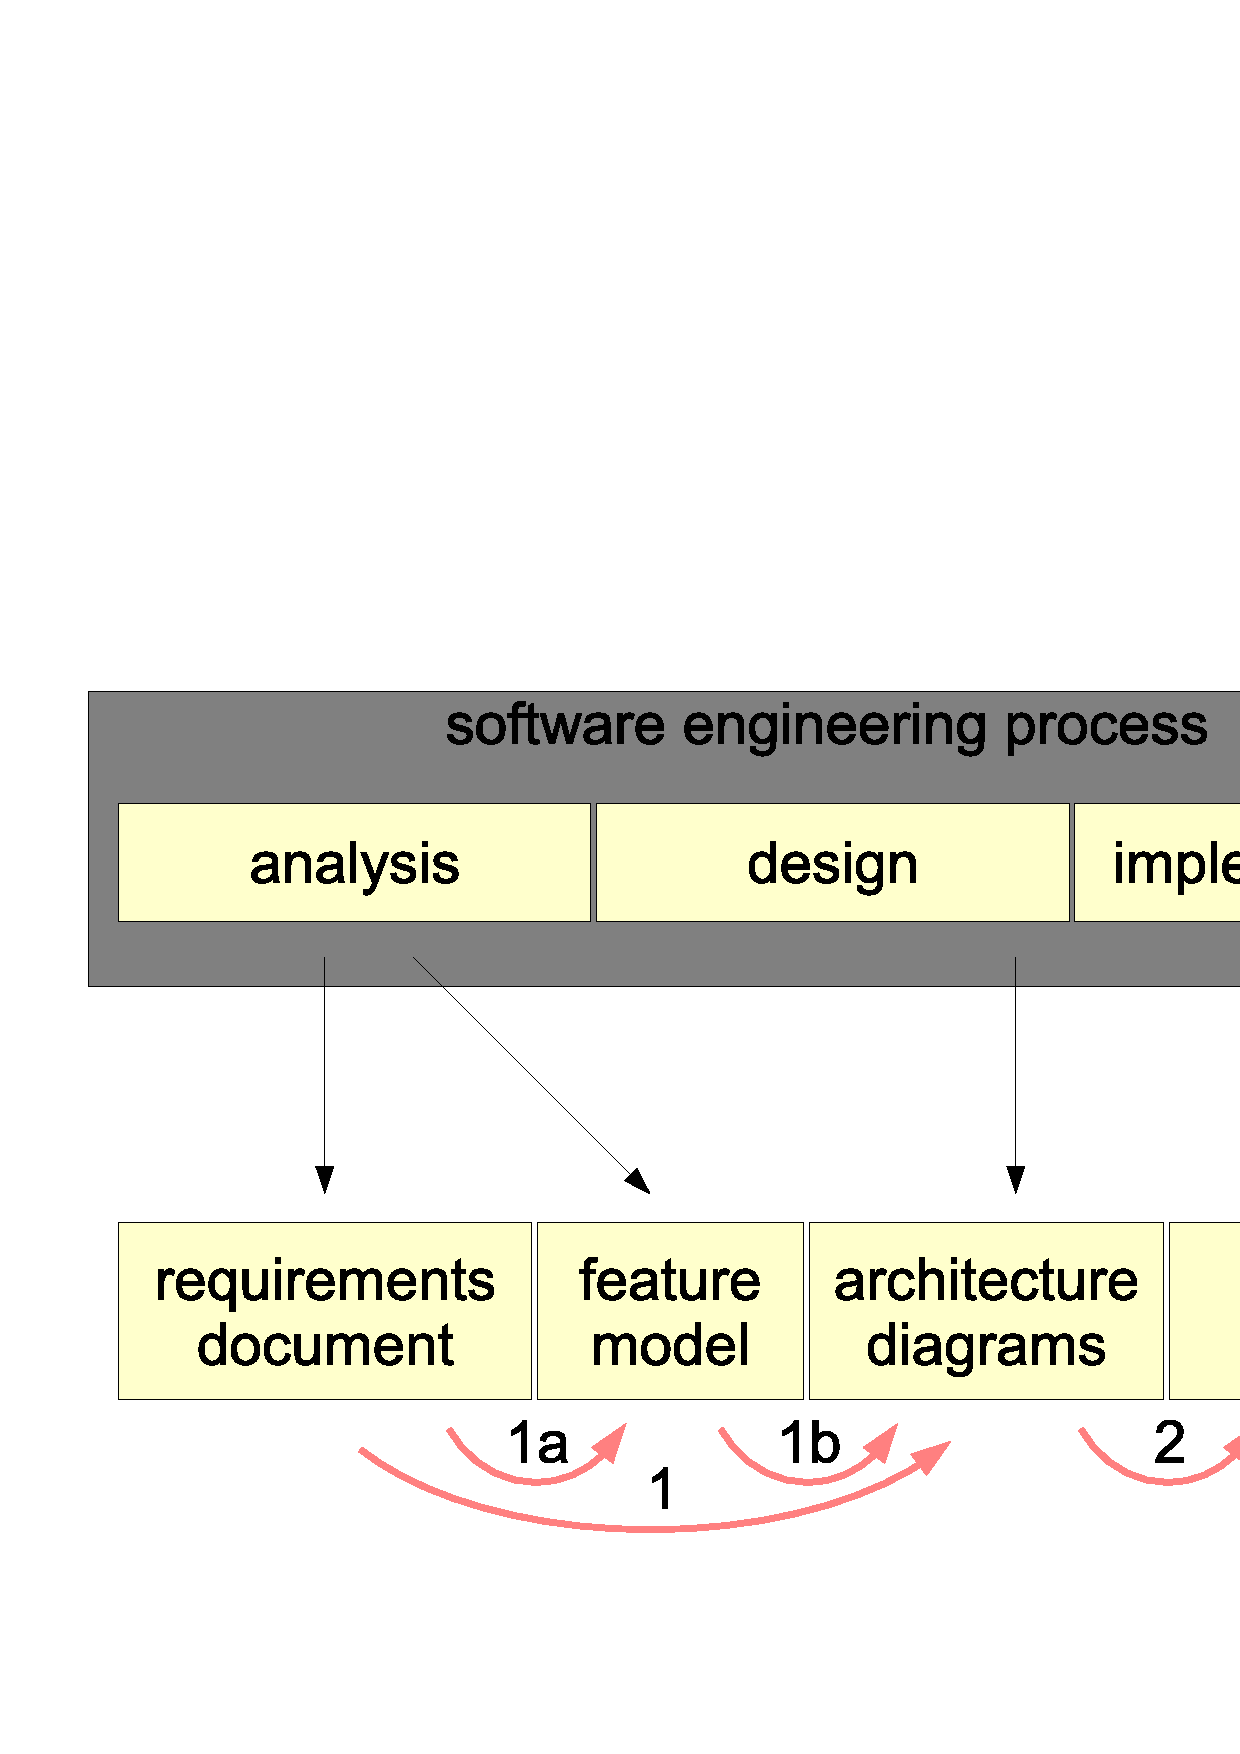
\includegraphics[scale=0.3,angle=-90]{graphics/gaps.pdf}
        \caption{Standard Software Engineering Process}
        \label{software_engineering_process_figure}
    \end{center}
\end{figure}
